\documentclass[10]{article}
%\documentclass[11pt]{book}
\usepackage{hyperref}
\usepackage{amsfonts,amssymb,amsmath,amsthm,cite}
\usepackage{lmodern, mathtools}
\usepackage{old-arrows} 
\usepackage{graphicx}
\usepackage[toc,page]{appendix}
\usepackage{nicefrac}
%% \usepackage[francais]{babel}
\usepackage[applemac]{inputenc}
\usepackage{amssymb, euscript}
\usepackage[matrix,arrow,curve]{xy}
\usepackage{graphicx}
\usepackage{tabularx}
\usepackage{float}
\usepackage{tikz}
\usepackage{slashed}
\usepackage{mathrsfs}
\usepackage{multirow}
%\usepackage{tikz-cd}

\usetikzlibrary{cd}

%\usepackage{mathtools}

\usetikzlibrary{matrix}

\usepackage[T1]{fontenc}
\usepackage{amsfonts,cite}
\usepackage{graphicx}

%% \usepackage[francais]{babel}
\usepackage[applemac]{inputenc}


\usepackage[sc]{mathpazo}
\usepackage{environ}

\linespread{1.05}         % Palatino needs more leading (space between lines)


%\usepackage[usenames]{color}



\DeclareFontFamily{T1}{pzc}{}
\DeclareFontShape{T1}{pzc}{m}{it}{1.8 <-> pzcmi8t}{}
\DeclareMathAlphabet{\mathpzc}{T1}{pzc}{m}{it}
% the command for it is \mathpzc

\textwidth=140mm


% % % % % % % % % % % % % % % % % % % %
\theoremstyle{plain}
\newtheorem{prop}{Proposition}[section]
\newtheorem{prdf}[prop]{Proposition and Definition}
\newtheorem{lem}[prop]{Lemma}%[section]
\newtheorem{cor}[prop]{Corollary}%[section]
\newtheorem{thm}[prop]{Theorem}%[section]
\newtheorem{theorem}[prop]{Theorem}
\newtheorem{lemma}[prop]{Lemma}
\newtheorem{proposition}[prop]{Proposition}
\newtheorem{corollary}[prop]{Corollary}
\newtheorem{statement}[prop]{Statement}

\theoremstyle{definition}
\newtheorem{defn}[prop]{Definition}%[section]
\newtheorem{cordefn}[prop]{Corollary and Definition}%[section]
\newtheorem{empt}[prop]{}%[section]
\newtheorem{exm}[prop]{Example}%[section]
\newtheorem{rem}[prop]{Remark}%[section]
\newtheorem{prob}[prop]{Problem}
\newtheorem{conj}{Conjecture}       %% Hypothesis 1
\newtheorem{cond}{Condition}        %% Condition 1
%\newtheorem{axiom}[thm]{Axiom}           %% Axiom 1 modified
\newtheorem{fact}[prop]{Fact}
\newtheorem{ques}{Question}         %% Question 1
\newtheorem{answ}{Answer}           %% Answer 1
\newtheorem{notn}{Notation}        %% Notations are not numbered

\theoremstyle{definition}
\newtheorem{notation}[prop]{Notation}
\newtheorem{definition}[prop]{Definition}
\newtheorem{example}[prop]{Example}
\newtheorem{exercise}[prop]{Exercise}
\newtheorem{conclusion}[prop]{Conclusion}
\newtheorem{conjecture}[prop]{Conjecture}
\newtheorem{criterion}[prop]{Criterion}
\newtheorem{summary}[prop]{Summary}
\newtheorem{axiom}[prop]{Axiom}
\newtheorem{problem}[prop]{Problem}
%\theoremstyle{remark}
\newtheorem{remark}[prop]{Remark}

\numberwithin{equation}{section}
\newtheorem*{claim}{Claim}
\DeclareMathOperator{\Dom}{Dom}              %% domain of an operator
\newcommand{\Dslash}{{D\mkern-11.5mu/\,}}    %% Dirac operator


%\newcommand\myeq{\stackrel{\mathclap{\normalfont\mbox{def}}}{=}}
\newcommand{\nor}[1]{\left\Vert #1\right\Vert}    %\nor{x}=||x||
\newcommand{\vertiii}[1]{{\left\vert\kern-0.25ex\left\vert\kern-0.25ex\left\vert #1
		\right\vert\kern-0.25ex\right\vert\kern-0.25ex\right\vert}}
\newcommand{\Ga}{\Gamma}  
\newcommand{\coker}{\mathrm{coker}}                   %% short for  \Gamma
\newcommand{\Coo}{C^\infty}                  %% smooth functions
% % % % % % % % % % % % % % % % % % % %


\usepackage[sc]{mathpazo}
\linespread{1.05}         % Palatino needs more leading (space between lines)

\newbox\ncintdbox \newbox\ncinttbox %% noncommutative integral symbols
\setbox0=\hbox{$-$} \setbox2=\hbox{$\displaystyle\int$}
\setbox\ncintdbox=\hbox{\rlap{\hbox
		to \wd2{\hskip-.125em \box2\relax\hfil}}\box0\kern.1em}
\setbox0=\hbox{$\vcenter{\hrule width 4pt}$}
\setbox2=\hbox{$\textstyle\int$} \setbox\ncinttbox=\hbox{\rlap{\hbox
		to \wd2{\hskip-.175em \box2\relax\hfil}}\box0\kern.1em}

\newcommand{\ncint}{\mathop{\mathchoice{\copy\ncintdbox}%
		{\copy\ncinttbox}{\copy\ncinttbox}%
		{\copy\ncinttbox}}\nolimits}  %% NC integral

%%% Repeated relations:
\newcommand{\xyx}{\times\cdots\times}      %% repeated product
\newcommand{\opyop}{\oplus\cdots\oplus}    %% repeated direct sum
\newcommand{\oxyox}{\otimes\cdots\otimes}  %% repeated tensor product
\newcommand{\wyw}{\wedge\cdots\wedge}      %% repeated exterior product
\newcommand{\subysub}{\subset\hdots\subset}      %% repeated subset
\newcommand{\supysup}{\supset\hdots\supset}      %% repeated supset
\newcommand{\rep}{\mathfrak{rep}}
\newcommand{\lift}{\mathfrak{lift}}
\newcommand{\desc}{\mathfrak{desc}}
%%% Roman letters:
\newcommand{\id}{\mathrm{id}}                %% identity map
\newcommand{\Id}{\mathrm{Id}}                %% identity map
\newcommand{\pt}{\mathrm{pt}}                %% a point
\newcommand{\const}{\mathrm{const}}          %% a constant
\newcommand{\codim}{\mathrm{codim}}          %% codimension
\newcommand{\cyc}{\mathrm{cyclic}}  %% cyclic sum
\renewcommand{\d}{\mathrm{d}}       %% commutative differential
\newcommand{\dR}{\mathrm{dR}}       %% de~Rham cohomology
\newcommand{\proj}{\mathrm{proj}}                %% a projection



\newcommand*{\Mult}{\mathcal M}% multiplier algebra

\newcommand{\A}{\mathcal{A}}                 %%\newcommand{\unitsv}[1]{#1^{(0)}}
\newcommand{\units}{G^{(0)}}
\newcommand{\haars}{\{\lambda^{u}\}_{u\in\units}}
\newcommand{\shaars}{\{\lambda_{u}\}_{u\in\units}}
\newcommand{\haarsv}[2]{\{\lambda^{#2}_{#1}\}_{#2\in\unitsv{#1}}}
\newcommand{\haarv}[2]{\lambda^{#2}_{#1}}

\renewcommand{\a}{\alpha}                    %% short for  \alphapha
\DeclareMathOperator{\ad}{ad}                %% infml adjoint repn
\newcommand{\as}{\quad\mbox{as}\enspace}     %% `as' with spacing
\newcommand{\Aun}{\widetilde{\mathcal{A}}}   %% unital algebra
\newcommand{\B}{\mathcal{B}}                 %% space of distributions
\newcommand{\E}{\mathcal{E}}                 %% space of distributions
\renewcommand{\b}{\beta}                     %% short for \beta
\newcommand{\braCket}[3]{\langle#1\mathbin|#2\mathbin|#3\rangle}
\newcommand{\braket}[2]{\langle#1\mathbin|#2\rangle} %% <w|z>
\newcommand{\C}{\mathbb{C}}                  %% complex numbers
\newcommand{\CC}{\mathcal{C}}                %% space of distributions
\newcommand{\cc}{\mathbf{c}}                 %% Hochschild cycle
\DeclareMathOperator{\Cl}{C\ell}             %% Clifford algebra
\newcommand{\F}{\mathcal{F}}                 %% space of test functions
\newcommand{\G}{\mathcal{G}}                 %% 
\newcommand{\D}{\mathcal{D}}                 %% Moyal L^2-filtration
\renewcommand{\H}{\mathcal{H}}               %% Hilbert space
\newcommand{\half}{\tfrac{1}{2}}             %% small fraction  1/2
\newcommand{\hh}{\mathcal{H}}                %% Hilbert space
\newcommand{\hookto}{\hookrightarrow}        %% abbreviation
\newcommand{\Ht}{{\widetilde{\mathcal{H}}}}  %% Hilbert space of forms
\newcommand{\I}{\mathcal{I}}                 %% tracelike functions
\DeclareMathOperator{\Junk}{Junk}            %% the junk DGA ideal
\newcommand{\K}{\mathcal{K}}                 %% compact operators
\newcommand{\ket}[1]{|#1\rangle}             %% ket vector
\newcommand{\ketbra}[2]{|#1\rangle\langle#2|} %% rank one operator
\renewcommand{\L}{\mathcal{L}}               %% operator algebra
\newcommand{\La}{\Lambda}                    %% short for \Lambda
\newcommand{\la}{\lambda}                    %% short for \lambda
\newcommand{\lf}{L_f^\theta}                 %% left mult operator
\newcommand{\M}{\mathcal{M}}                 %% Moyal multplr algebra
\newcommand{\mm}{\mathcal{M}^\theta}
%\newcommand{{{\star_{\theta}}}{{\mathchoice{\mathbin{\;|\;ar_{_\theta}}}
			%            {\mathbin{\;|\;ar_{_\theta}}}           %% Moyal
			%            {{\;|\;ar_\theta}}{{\;|\;ar_\theta}}}}    %% product
	\newcommand{\N}{\mathbb{N}}                  %% nonnegative integers
	\newcommand{\NN}{\mathcal{N}}                %% a Moyal algebra
	\newcommand{\nb}{\nabla}                     %% gradient
	\newcommand{\Oh}{\mathcal{O}}                %% comm multiplier alg
	\newcommand{\om}{\omega}                     %% short for \omega
	\newcommand{\opp}{{\mathrm{op}}}             %% opposite algebra
	\newcommand{\ox}{\otimes}                    %% tensor product
	\newcommand{\eps}{\varepsilon}                    %% tensor product
	\newcommand{\otimesyox}{\otimes\cdots\otimes}    %% repeated tensor product
	\newcommand{\pa}{\partial}                   %% short for \partial
	\newcommand{\pd}[2]{\frac{\partial#1}{\partial#2}}%% partial derivative
	\newcommand{\piso}[1]{\lfloor#1\rfloor}      %% integer part
	\newcommand{\PsiDO}{\Psi~\mathrm{DO}}         %% pseudodiffl operators
	\newcommand{\Q}{\mathbb{Q}}                  %% rational numbers
	\newcommand{\R}{\mathbb{R}}                  %% real numbers
	\newcommand{\rdl}{R_\Dslash(\lambda)}        %% resolvent
	\newcommand{\roundbraket}[2]{(#1\mathbin|#2)} %% (w|z)
	\newcommand{\row}[3]{{#1}_{#2},\dots,{#1}_{#3}} %% list: a_1,...,a_n
	\newcommand{\sepword}[1]{\quad\mbox{#1}\quad} %% well-spaced words
	\newcommand{\set}[1]{\{\,#1\,\}}             %% set notation
	\newcommand{\Sf}{\mathbb{S}}                 %% sphere
	\newcommand{\uhor}[1]{\Omega^1_{hor}#1}
	\newcommand{\sco}[1]{{\sp{(#1)}}}
	\newcommand{\sw}[1]{{\sb{(#1)}}}
	\DeclareMathOperator{\spec}{sp}              %% spectrum
	\renewcommand{\SS}{\mathcal{S}}              %% Schwartz space
	\newcommand{\sss}{\mathcal{S}}               %% Schwartz space
	\DeclareMathOperator{\supp}{\mathfrak{supp}}            %% support
	\newcommand{\T}{\mathbb{T}}                  %% circle as a group
	\renewcommand{\th}{\theta}                   %% short for \theta
	\newcommand{\thalf}{\tfrac{1}{2}}            %% small* fraction 1/2
	\newcommand{\tihalf}{\tfrac{i}{2}}           %% small* fraction i/2
	\newcommand{\tpi}{{\tilde\pi}}               %% extended representation
	\DeclareMathOperator{\Tr}{Tr}                %% trace of operator
	\DeclareMathOperator{\tr}{tr}                %% trace of matrix
	\newcommand{\del}{\partial}                  %% short for  \partial
	\DeclareMathOperator{\tsum}{{\textstyle\sum}} %% small sum in display
	\newcommand{\V}{\mathcal{V}}                 %% test function space
	\newcommand{\vac}{\ket{0}}                   %% vacuum ket vector
	\newcommand{\vf}{\varphi}                    %% scalar field
	\newcommand{\w}{\wedge}                      %% exterior product
	\DeclareMathOperator{\wres}{wres}            %% density of Wresidue
	\newcommand{\x}{\times}                      %% cross
	\newcommand{\Z}{\mathbb{Z}}                  %% integers
	\newcommand{\7}{\dagger}                     %% short for + symbol
	\newcommand{\8}{\bullet}                     %% anonymous degree
	\renewcommand{\.}{\cdot}                     %% anonymous variable
	\renewcommand{\:}{\colon}                    %% colon in  f: A -> B
	
	%\newcommand{\sA}{\mathscr{A}}       %%
	\newcommand{\sA}{\mathcal{A}} 
	\newcommand{\sB}{\mathcal{B}}       %%
	\newcommand{\sC}{\mathcal{C}}       %%
	\newcommand{\sD}{\mathcal{D}}       %%
	\newcommand{\sE}{\mathcal{E}}       %%
	\newcommand{\sF}{\mathcal{F}}       %%
	\newcommand{\sG}{\mathcal{G}}       %%
	\newcommand{\sH}{\mathcal{H}}       %%
	\newcommand{\sI}{\mathcal{I}}       %%
	\newcommand{\sJ}{\mathcal{J}}       %%
	\newcommand{\sK}{\mathcal{K}}       %%
	\newcommand{\sL}{\mathcal{L}}       %%
	\newcommand{\sM}{\mathcal{M}}       %%
	\newcommand{\sN}{\mathcal{N}}       %%
	\newcommand{\sO}{\mathcal{O}}       %%
	\newcommand{\sP}{\mathcal{P}}       %%
	\newcommand{\sQ}{\mathcal{Q}}       %%
	\newcommand{\sR}{\mathcal{R}}       %%
	\newcommand{\sS}{\mathcal{S}}       %%
	\newcommand{\sT}{\mathcal{T}}       %%
	\newcommand{\sU}{\mathcal{U}}       %%
	\newcommand{\sV}{\mathcal{V}}       %%
	\newcommand{\sX}{\mathcal{X}}       %%
	\newcommand{\sY}{\mathcal{Y}}       %%
	\newcommand{\sZ}{\mathcal{Z}}       %%
	
	\newcommand{\Om}{\Omega}       %%
	
	
	\DeclareMathOperator{\ptr}{ptr}     %% Poisson trace
	\DeclareMathOperator{\Trw}{Tr_\omega} %% Dixmier trace
	\DeclareMathOperator{\vol}{Vol}     %% total volume
	\DeclareMathOperator{\Vol}{Vol}     %% total volume
	\DeclareMathOperator{\Area}{Area}   %% area of a surface
	\DeclareMathOperator{\Wres}{Wres}   %% (Wodzicki) residue
	
	\newcommand{\dd}[1]{\frac{\partial}{\partial#1}}   %% partial derivation
	\newcommand{\ddt}[1]{\frac{d}{d#1}}                %% derivative
	\newcommand{\inv}[1]{\frac{1}{#1}}                 %% inverse
	\newcommand{\sfrac}[2]{{\scriptstyle\frac{#1}{#2}}} %% tiny fraction
	
	\newcommand{\bA}{\mathbb{A}}       %%
	\newcommand{\bB}{\mathbb{B}}       %%
	\newcommand{\bC}{\mathbb{C}}       %%
	\newcommand{\bCP}{\mathbb{C}P}     %%
	\newcommand{\bD}{\mathbb{D}}       %%
	\newcommand{\bE}{\mathbb{E}}       %%
	\newcommand{\bF}{\mathbb{F}}       %%
	\newcommand{\bG}{\mathbb{G}}       %%
	\newcommand{\bH}{\mathbb{H}}       %%
	\newcommand{\bHP}{\mathbb{H}P}     %%
	\newcommand{\bI}{\mathbb{I}}       %%
	\newcommand{\bJ}{\mathbb{J}}       %%
	\newcommand{\bK}{\mathbb{K}}       %%
	\newcommand{\bL}{\mathbb{L}}       %%
	\newcommand{\bM}{\mathbb{M}}       %%
	\newcommand{\bN}{\mathbb{N}}       %%
	\newcommand{\bO}{\mathbb{O}}       %%
	\newcommand{\bOP}{\mathbb{O}P}     %%
	\newcommand{\bP}{\mathbb{P}}       %%
	\newcommand{\bQ}{\mathbb{Q}}       %%
	\newcommand{\bR}{\mathbb{R}}       %%
	\newcommand{\bRP}{\mathbb{R}P}     %%
	\newcommand{\bS}{\mathbb{S}}       %%
	\newcommand{\bT}{\mathbb{T}}       %%
	\newcommand{\bU}{\mathbb{U}}       %%
	\newcommand{\bV}{\mathbb{V}}       %%
	\newcommand{\bX}{\mathbb{X}}       %%
	\newcommand{\bY}{\mathbb{Y}}       %%
	\newcommand{\bZ}{\mathbb{Z}}       %%
	
	\newcommand{\bydef}{\stackrel{\mathrm{def}}{=}}          %% 
	
	
	\newcommand{\al}{\alpha}          %% short for  \alpha
	\newcommand{\bt}{\beta}           %% short for  \beta
	\newcommand{\Dl}{\Delta}          %% short for  \Delta
	\newcommand{\dl}{\delta}          %% short for  \delta
	\newcommand{\ga}{\gamma}          %% short for  \gamma
	\newcommand{\ka}{\kappa}          %% short for  \kappa
	\newcommand{\sg}{\sigma}          %% short for  \sigma
	\newcommand{\Sg}{\Sigma}          %% short for  \Sigma
	\newcommand{\Th}{\Theta}          %% short for  \Theta
	\renewcommand{\th}{\theta}        %% short for  \theta
	\newcommand{\vth}{\vartheta}      %% short for  \vartheta
	\newcommand{\ze}{\zeta}           %% short for  \zeta
	
	\DeclareMathOperator{\ord}{ord}     %% order of a PsiDO
	\DeclareMathOperator{\rank}{rank}   %% rank of a vector bundle
	\DeclareMathOperator{\sign}{sign}   %%
	\DeclareMathOperator{\sgn}{sgn}   %%
	\DeclareMathOperator{\chr}{char}   %%
	\DeclareMathOperator{\ev}{ev}       %% evaluation
	
	
	\newcommand{\Op}{\mathbf{Op}}
	\newcommand{\As}{\mathbf{As}}
	\newcommand{\Com}{\mathbf{Com}}
	\newcommand{\LLie}{\mathbf{Lie}}
	\newcommand{\Leib}{\mathbf{Leib}}
	\newcommand{\Zinb}{\mathbf{Zinb}}
	\newcommand{\Poiss}{\mathbf{Poiss}}
	
	\newcommand{\gX}{\mathfrak{X}}      %% vector fields
	\newcommand{\sol}{\mathfrak{so}}    %% special orthogonal Lie algebra
	\newcommand{\gm}{\mathfrak{m}}      %% maximal ideal
	
	
	\DeclareMathOperator{\Res}{Res}
	\DeclareMathOperator{\NCRes}{NCRes}
	\DeclareMathOperator{\Ind}{Ind}
	%% co/homology theories
	\DeclareMathOperator{\rH}{H}        %% any co/homology
	\DeclareMathOperator{\rC}{C}        %%  any co/chains
	\DeclareMathOperator{\rZ}{Z}        %% cycles
	\DeclareMathOperator{\rB}{B}        %% boundaries
	\DeclareMathOperator{\rF}{F}        %% filtration
	\DeclareMathOperator{\Gr}{gr}        %% associated graded object
	\DeclareMathOperator{\rHc}{H_{\mathrm{c}}}   %% co/homology with compact support
	\DeclareMathOperator{\drH}{H_{\mathrm{dR}}}  %% de Rham co/homology
	\DeclareMathOperator{\cechH}{\check{H}}    %% Cech co/homology
	\DeclareMathOperator{\rK}{K}        %% K-groups
	\DeclareMathOperator{\rKO}{KO}        %% real K-groups
	\DeclareMathOperator{\rKU}{KU}        %% unitary K-groups
	\DeclareMathOperator{\rKSp}{KSp}        %% symplectic K-groups
	\DeclareMathOperator{\rR}{R}        %% representation ring
	\DeclareMathOperator{\rI}{I}        %% augmentation ideal
	\DeclareMathOperator{\HH}{HH}       %% Hochschild co/homology
	\DeclareMathOperator{\HC}{HC}       %% cyclic co/homology
	\DeclareMathOperator{\HP}{HP}       %% periodic cyclic co/homology
	\DeclareMathOperator{\HN}{HN}       %% negative cyclic co/homology
	\DeclareMathOperator{\HL}{HL}       %% Leibniz co/homology
	\DeclareMathOperator{\KK}{KK}       %% KK-theory
	\DeclareMathOperator{\KKK}{\mathbf{KK}}       %% KK-theory as a category
	\DeclareMathOperator{\Ell}{Ell}       %% Abstract elliptic operators
	\DeclareMathOperator{\cd}{cd}       %% cohomological dimension
	\DeclareMathOperator{\spn}{span}       %% span
	\DeclareMathOperator{\linspan}{span} %% linear span (can't use \span)
	\newcommand{\blank}{-}   
	
	
	
	\newcommand{\twobytwo}[4]{\begin{pmatrix} #1 & #2 \\ #3 & #4 \end{pmatrix}}
	\newcommand{\CGq}[6]{C_q\!\begin{pmatrix}#1&#2&#3\\#4&#5&#6\end{pmatrix}}
	%% q-Clebsch--Gordan coefficients
	\newcommand{\cz}{{\bullet}}         %% anonymous degree
	\newcommand{\nic}{{\vphantom{\dagger}}} %% invisible dagger
	\newcommand{\ep}{{\dagger}}         %% abbreviation for + symbol
	\newcommand{\downto}{\downarrow}    %% right hand limit
	\newcommand{\isom}{\cong}          %% isomorphism
	\newcommand{\lt}{\triangleright}    %% a left action
	\newcommand{\otto}{\leftrightarrow} %% bijection
	\newcommand{\rt}{\triangleleft}     %% a right action
	\newcommand{\semi}{\rtimes}         %% crossed product
	\newcommand{\tensor}{\otimes}       %% tensor product
	\newcommand{\cotensor}{\square}       %% cotensor product
	\newcommand{\trans}{\pitchfork}     %% transverse
	\newcommand{\ul}{\underline}        %% for sheaves
	\newcommand{\upto}{\uparrow}        %% left hand limit
	\renewcommand{\:}{\colon}           %% colon in  f: A -> B
	\newcommand{\blt}{\ast}
	\newcommand{\Co}{C_{\bullet}}
	\newcommand{\cCo}{C^{\bullet}}
	\newcommand{\nbs}{\nabla^S}         %% spin connection
	\newcommand{\up}{{\mathord{\uparrow}}} %% `up' spinors
	\newcommand{\dn}{{\mathord{\downarrow}}} %% `down' spinors
	\newcommand{\updn}{{\mathord{\updownarrow}}} %% up or down
	
	%%% Bilinear enclosures:
	
	\newcommand{\bbraket}[2]{\langle\!\langle#1\stroke#2\rangle\!\rangle}
	%% <<w|z>>
	\newcommand{\bracket}[2]{\langle#1,\, #2\rangle} %% <w,z>
	\newcommand{\scalar}[2]{\langle#1,\,#2\rangle} %% <w,z>
	\newcommand{\poiss}[2]{\{#1,\,#2\}} %% {w,z}
	\newcommand{\dst}[2]{\langle#1,#2\rangle} %% distributions <u,\phi>
	\newcommand{\pairing}[2]{(#1\stroke #2)} %% right-linear pairing
	\def\<#1|#2>{\langle#1\stroke#2\rangle} %% \braket (Dirac notation)
	\def\?#1|#2?{\{#1\stroke#2\}}        %% left-linear pairing
	
	%%% Accent-like macros:
	
	\renewcommand{\Bar}[1]{\overline{#1}} %% closure operator
	\renewcommand{\Hat}[1]{\widehat{#1}}  %% short for \widehat
	\renewcommand{\Tilde}[1]{\widetilde{#1}} %% short for \widetilde
	
	
	\DeclareMathOperator{\bCl}{\bC l}   %% complex Clifford algebra
	
	%%% Small fractions in displays:
	
	\newcommand{\ihalf}{\tfrac{i}{2}}   %% small fraction  i/2
	\newcommand{\quarter}{\tfrac{1}{4}} %% small fraction  1/4
	\newcommand{\shalf}{{\scriptstyle\frac{1}{2}}}  %% tiny fraction  1/2
	\newcommand{\third}{\tfrac{1}{3}}   %% small fraction  1/3
	\newcommand{\ssesq}{{\scriptstyle\frac{3}{2}}} %% tiny fraction  3/2
	\newcommand{\sesq}{{\mathchoice{\tsesq}{\tsesq}{\ssesq}{\ssesq}}} %% 3/2
	\newcommand{\tsesq}{\tfrac{3}{2}}   %% small fraction  3/2
	
	
	%\newcommand\eqdef{\overset{\mathclap{\normalfont\mbox{def}}}{=}}
	\newcommand\eqdef{\overset{\mathrm{def}}{=}}
	
	
	%+++++++++++++++++++++++++++++++++++
	
	\newcommand{\word}[1]{\quad\text{#1}\enspace} %% well-spaced words
	\newcommand{\words}[1]{\quad\text{#1}\quad} %% better-spaced words
	\newcommand{\su}[1]{{\sp{[#1]}}}
	
	\def\<#1,#2>{\langle#1,#2\rangle}            %% bilinear pairing
	\def\ee_#1{e_{{\scriptscriptstyle#1}}}       %% basis projector
	\def\wick:#1:{\mathopen:#1\mathclose:}       %% Wick-ordered operator
	
	\newcommand{\opname}[1]{\mathop{\mathrm{#1}}\nolimits}
	
	\newcommand{\hideqed}{\renewcommand{\qed}{}} %% to suppress `\qed'
	
	
	%%%%%%%%%%%%%%%%%%%%%%%%%%%%%
	%% 2. Some internal machinery
	%%%%%%%%%%%%%%%%%%%%%%%%%%%%%
	
	\newbox\ncintdbox \newbox\ncinttbox %% noncommutative integral symbols
	\setbox0=\hbox{$-$}
	\setbox2=\hbox{$\displaystyle\int$}
	\setbox\ncintdbox=\hbox{\rlap{\hbox
			to \wd2{\box2\relax\hfil}}\box0\kern.1em}
	\setbox0=\hbox{$\vcenter{\hrule width 4pt}$}
	\setbox2=\hbox{$\textstyle\int$}
	\setbox\ncinttbox=\hbox{\rlap{\hbox
			to \wd2{\hskip-.05em\box2\relax\hfil}}\box0\kern.1em}
	
	\newcommand{\disp}{\displaystyle} %% short for  \displaystyle
	
	%\newcommand{\hideqed}{\renewcommand{\qed}{}} %% no `\qed' at end-proof
	
	\newcommand{\stroke}{\mathbin|}   %% (for `\bbraket' and such)
	\newcommand{\tribar}{|\mkern-2mu|\mkern-2mu|} %% norm bars: |||
	
	%%% Enclose one argument with delimiters:
	
	\newcommand{\bra}[1]{\langle{#1}\rvert} %% bra vector <w|
	\newcommand{\kett}[1]{\lvert#1\rangle\!\rangle} %% ket 2-vector |y>>
	\newcommand{\snorm}[1]{\mathopen{\tribar}{#1}%
		\mathclose{\tribar}}                 %% norm |||x|||
	
	
	\newcommand{\End}{\mathrm{End}}       %%
	\newcommand{\Ext}{\mathrm{Ext}}       %%
	\newcommand{\Hom}{\mathrm{Hom}}       %%
	\newcommand{\Mrt}{\mathrm{Mrt}}       %%
	\newcommand{\grad}{\mathrm{grad}}       %%
	\newcommand{\Spin}{\mathrm{Spin}}       %%
	\newcommand{\Ad}{\mathrm{Ad}}       %%
	\newcommand{\Pic}{\mathrm{Pic}}       %%
	\newcommand{\Aut}{\mathrm{Aut}}       %%
	\newcommand{\Inn}{\mathrm{Inn}}       %%
	\newcommand{\Out}{\mathrm{Out}}       %%
	\newcommand{\Homeo}{\mathrm{Homeo}}       %%
	\newcommand{\Diff}{\mathrm{Diff}}       %%
	\newcommand{\im}{\mathrm{im}}       %%
	
	
	\newcommand{\SO}{\mathrm{SO}}       %%
	\newcommand{\SU}{SU}       %%
	\newcommand{\gso}{\mathfrak{so}}    %% special orthogonal Lie algebra
	\newcommand{\gero}{\mathfrak{o}}    %% orthogonal Lie algebra
	\newcommand{\gspin}{\mathfrak{spin}} %% spin Lie algebra
	\newcommand{\gu}{\mathfrak{u}}      %% unitary Lie algebra
	\newcommand{\gsu}{\mathfrak{su}}    %% special unitary Lie algebra
	\newcommand{\gsl}{\mathfrak{sl}}    %% special linear Lie algebra
	\newcommand{\gsp}{\mathfrak{sp}}    %% symplectic linear Lie algebra
	
	%\newcommand{\bes}{\begin{equation}\begin{split}}
			%\newcommand{\ees}{\end{split}\end{equation}}
	%\NewEnviron{split.enviro}{%
		%	\begin{equation}\begin{split}
				%	\BODY
				%	\end{split}\end{equation}
		%$}
	\newenvironment{splitequation}{\begin{equation}\begin{split}}{\end{split}\end{equation}}
	
	%Begin equation split: Begin equation split = bes
	\newcommand{\bs}{\begin{split}}
		\newcommand{\es}{\end{split}}
	\newcommand{\be}{\begin{equation}}
		\renewcommand{\ee}{\end{equation}}
	\newcommand{\bea}{\begin{eqnarray}}
		\newcommand{\eea}{\end{eqnarray}}
	\newcommand{\bean}{\begin{eqnarray*}}
		\newcommand{\eean}{\end{eqnarray*}}
	\newcommand{\brray}{\begin{array}}
		\newcommand{\erray}{\end{array}}
	\newenvironment{equations}
	{\begin{equation}
			\begin{split}}
			{\end{split}
	\end{equation}}
	\newcommand{\Hsquare}{%
		\text{\fboxsep=-.2pt\fbox{\rule{0pt}{1ex}\rule{1ex}{0pt}}}%
	}
	\makeatletter
	\newcommand{\xdbheadrightarrow}[2][]{%
		\ext@arrow 0099\xdbheadfill@{#1}{#2}}%
	\newcommand{\xdbheadfill@}{%
		\arrowfill@\relbar\relbar{\mathrel{\vphantom{\rightarrow}\smash{\twoheadrightarrow}}}}
	\makeatother
	
	%\xdbheadrightarrow
	
	\title{Grothendieck topology of  $C^*$-algebras}
	
	\author
	{\textbf{Petr R. Ivankov*}\\
		e-mail: * monster.ivankov@gmail.com \\
	}
	
	\begin{document}

\maketitle  %\setlength{\parindent}{0pt}
\pagestyle{plain}


%\vspace{1 in}


%\noindent

\begin{abstract}
For any topological space there is a sheaf cohomology. A Grothendieck topology  is a generalization  of the  classical topology such that  it also possesses a sheaf cohomology. On the other hand any noncommutative $C^*$-algebra is a generalization of a locally compact Hausdorff space. Here we define a Grothendieck topology arising from  $C^*$-algebras which is a generalization of the topology of the spectra of commutative $C^*$-algebras. This construction yields a noncommutative generalization of the sheaf cohomology of topological spaces.  The presented here theory gives a unified approach to  the  Gelfand duality and the duality between the commutative von Neumann algebras and measure locales.  The generalization of the  Dixmier-Douady theory  concerning $C^*$-algebras of foliations is also discussed.  

\end{abstract}


%\end{abstract}

\section{General theory}
\subsection{Grothendieck topology}
\paragraph*{}

	If $A$ is a $C^*$-algebra then there is a category $\mathbf{Hered}/A$ such that:
\begin{itemize}
	\item $\mathbf{Hered}/A$-objects are hereditary $C^*$- subalgebras of $A$,
	\item $\mathbf{Hered}/A$-morphism  from $B' \subset A$ to $B'' \subset A$ is a natural inclusion $B'\subset B''$ such that a following diagram 
	\newline
	\begin{tikzpicture}
		\matrix (m) [matrix of math nodes,row sep=3em,column sep=4em,minimum width=2em]
		{
			B'  &  & B''\\ 
			& A &\\};
		\path[-stealth]
		(m-1-1) edge node [above] {$\subset$} (m-1-3)
		(m-1-1) edge node [above]  {} (m-2-2)
		(m-1-3) edge node [right]  {} (m-2-2);
	\end{tikzpicture}
	\\
	is commutative.
\end{itemize}
For any two $\mathbf{Hered}/A$-objects $B', B''$ we define their \textit{fibre product} (cf. Definition \ref{pullback_defn}) by the following way
$$
B'\times_A B'' \bydef B'\cap B''.
$$

\begin{definition}\label{hered_cov_defn}
For any $\mathbf{Hered}/A$-object $B$ a distinguished set of families of inclusions $\left\{B_\iota \subset B\right\}_{\iota\in I}$, called a \textit{covering} of $B$ if $B$ is a generated by the union $\cup B_\iota$ hereditary $C^*$-subalgebra of $A$ (cf. Definition \ref{hered_generated_defn}).
\end{definition}

\begin{lemma}\label{grothendieck_ca_lem}
A given by the Definition \ref{hered_cov_defn} system of coverings satisfies to  the Definition \ref{pretopology_defn}, so one has a natural Grothendieck pretopology.
\end{lemma}
\begin{proof}
	If $A$ be a $C^*$-algebra, then one needs check that hereditary $C^*$-subalgebras of $A$ satisfy to axioms (a)-(c) of the Definition \ref{pretopology_defn}!.\\
	(a) Let $B, C\subset A$ be subalgebras. A covering of $B$ is a family $\left\{B_\iota\subset B\right\}_{\iota \in I}$ of hereditary subalgebras of $B$ such that $B$ is a generated by a union $\bigcup B_\iota$ hereditary $C^*$-subalgebra (cf. Definition \ref{hered_generated_defn}). If  $L\left( B\right)$, $L\left( C\right)$ and $L\left( B_\iota \right)$ are given by the equation \eqref{left_ideal_eqn} closed left ideals then $L\left(B\cap C \right) = L(B)\cap L(C)$, $~L\left(B_\iota \cap C \right)= L\left(B_\iota \right)\cap L\left( C \right)$ (cf. Lemma \ref{hered_ideal_lem}). Moreover $L\left(B\right)$ is the $C^*$-norm closure of an algebraic sum $\sum_{\iota\in I} L\left( B_\iota\right)$. For any $\iota \in I$ one has $L\left(B_\iota\right)\cap L\left(C\right)\subset L\left(B\right)\cap L\left(C\right)$ it follows that $\sum_{\iota\in I} \left( L\left(B_\iota\right)\cap L\left(C\right)\right) \subset L\left(B\right)\cap L\left(C\right)$. Since the left ideal  $L\left(B\right)\cap L\left(C\right)$ is $C^*$-norm closed the $C^*$-norm closure of an algebraic sum $\sum_{\iota\in I} \left( L\left(B_\iota\right)\cap L\left(C\right)\right)$ is a subset of  the intersection $L\left(B\right)\cap L\left(C\right)$ i.e. a generated by a union $\cup_\iota \left( B_\iota\cup C\right)$ hereditary subalgebra is a subalgebra of the intersection $B\cap C$. If $\eps > 0$ and $ b\in L\left(C\right)\cap L\left(B\right)$ then from the from the Theorem \ref{left_ideal_thm} it follows that there is a positive $u \in L\left(C\right)$ such that 
	\bean
	\left\|u \right\| \le 1,\\
	\left\|b - b u\right\|< \frac{\eps}{2}.
	\eean 
	Since the set $\sum_{\iota\in I}  L\left(B_\iota\right)$ is dense in $L\left(B\right)$ there is a sum $\sum_{k = 1}^n b_{k}$ such that
	\bean
	\forall k\in \{1,..., n\}\quad \exists \iota_k\in I \quad b_k \in L\left( B_{\iota_k}\right)  ,\\
		\left\|b - \sum_{k = 1}^n b_k \right\|< \frac{\eps}{2}.
		\eean
		Applying the triangle identity one has
	$$
	\left\|b -  \left( \sum_{k = 1}^n b_k\right)  u\right\|	\le 	\left\|\left( b -   \sum_{k = 1}^n b_k\right)  u\right\|+ \left\|b -   b  u\right\|< \left\| b -   \sum_{k = 1}^n b_k\right\|\left\|  u\right\|+ \frac{\eps}{2}< \eps.
$$
From the following circumstances:
\begin{itemize}
	\item  the number $\eps$ is arbitrary small,
	\item $\left( \sum_{k = 1}^n b_k\right)  u\in \sum_{\iota\in I} \left( L\left(B_\iota\right)\cap L\left(C\right)\right)$
\end{itemize}
we conclude that $b$ lies in the $C^*$-norm closure of $\sum_{\iota\in I} \left( L\left(B_\iota\right)\cap L\left(C\right)\right)$. So $L\left(B\right)\cap L\left(C\right)$ equals to the $C^*$-norm closure of $\sum_{\iota\in I} \left( L\left(B_\iota\right)\cap L\left(C\right)\right)$ and $B\cap C$ is a generated by the union $\cup_{\iota\in I} \left(B_\iota\cap C \right)$ hereditary $C^*$-algebra. Thus 
	a family $\left\{B_\iota\cap C \subset B\cap C\right\}_{\iota\in I}$ is a {covering} of $B\cap C$ (cf. Definition \ref{hered_cov_defn}).
	\\
	(b) If a family $\left\{B_\iota\subset B\right\}_{\iota\in I}$ is a covering of $B$ and for all $\iota$ a family $\left\{C_{\iota j}\subset B_\iota \right\}_{j\in J_\iota}$ is a covering of $B_\iota$ then  one has:
	\begin{itemize}
		\item The given by the equation \eqref{left_ideal_eqn}  closed left ideal $L\left( B\right)$ is the $C^*$-norm closure of an algebraic sum  $\sum_{\iota\in I} L\left( B_\iota \right)$, 
		\item for all $\iota\in I$ the left ideal  $L\left( B_\iota \right)$ is  the $C^*$-norm closure of an algebraic sum  $\sum_{j\in J_\iota} L\left( C_{\iota j} \right)$.
	\end{itemize}
	From $\sum_{\iota\in I} L\left( B_\iota \right)\subset L\left(B \right)$ and $\sum_j L\left( C_{\iota_j} \right)\subset L\left(B_\iota \right)$ for any $\iota \in I$ it follows that $\sum_{\iota j} L\left( C_{\iota_j} \right)\subset L\left(B \right)$. However the ideal $ L\left(B \right)$ is $C^*$-norm closed so a $C^*$-norm closure of $\sum_{\iota j} L\left( C_{\iota_j} \right)$ is a subset of $ L\left(B \right)$. 
	For all $b \in L\left( B\right)$ and  $\eps > 0$	there is a sum $\sum_{k = 1}^n b_{k}$ such that
	\bean
	\forall k\in \{1,..., n\}\quad \exists \iota_k\in I \quad b_k \in L\left( B_{\iota_k}\right) ,\\
	\left\|b - \sum_{k = 1}^n b_k \right\|< \frac{\eps}{2}.
	\eean
	For all $k \in \{1,...,n\}$ there is a sum $\sum_{l = 1}^{m_k} c_{k l}$ such that
	\bean
	\forall l\in \{1,..., {m_k}\}\quad \exists j_l \in J_\iota  \quad c_l \in L\left( C_{\iota_k j_l}\right) ,\\
	\left\|b_k - \sum_{l = 1}^{m_k} c_{\iota l} \right\|< \frac{\eps}{2n}.
	\eean
From these facts it follows that if
$$
b' \bydef \sum_{k = 1}^n \sum_{l = 1}^{m_k} c_{k l}
$$
then
\bean
b' \in \sum_{\iota j} L\left( C_{\iota j}\right) ,\\
\left\|b - b' \right\| < \eps.
\eean	
The element $b$ lies in the $C^*$-norm closure of the algebraic sum $\sum_{\iota j}L\left(  C_{\iota j}\right) $ because the number $\eps$ is arbitrary small, so $L\left(B \right)$ is the $C^*$-norm closure of the algebraic sum $\sum_{\iota j}L\left(  C_{\iota j}\right)$. Taking into account  the Lemma \ref{hered_ideal_lem} one can deduce that $B$ is a generated by a union $\cup_{\iota j}  C_{\iota j}$ hereditary subalgebra (cf. Definition \ref{hered_generated_defn}), i.e. 
	a family $\left\{C_{\iota j} \subset B\right\}$ is a {covering} of $B$.
	\\
	(c) Evident.
\end{proof}
\begin{empt}\label{grothendieck_ca_empt}
	From the Remark \ref{pretopology_to_topology_rem} it follows that the given by the Lemma \ref{grothendieck_ca_lem} Grothendieck pretopology can be replaced by the natural Grothendieck topology $J_A$ (cf Definition \ref{grotendieck_topolgy_defn}).
\end{empt}
\begin{definition}\label{grothendieck_ca_defn}
The explained in  \ref{grothendieck_ca_empt} Grothendieck topology $J_A$  is said to be a  \textit{Gelfand} $A$-\textit{topology}. A corresponding  site (cf. Definition \ref{grotendieck_topolgy_defn}) $\mathbf{T}_A\bydef \left(\mathbf{Hered}/A, J_A\right)$ is said to be \textit{arising} from $A$ (cf. Definition \ref{top_gro_definition}). A Grothendieck topos $\mathfrak{Topos}(A)\bydef \mathbf{Sh}\left(\mathbf{T}_A \right)$ is said to be the \textit{Hereditary} $A$-\textit{topos}.
\end{definition}
\begin{remark}\label{locale_rem}
From the proof of the Theorem \ref{hered_cov_defn} it follows that there is a frame (cf. Definition \ref{locale_defn}) such that
\be\label{locale_eqn}
\begin{split}
\bigvee_{\iota\in I} B_\iota \bydef \text{ a generated by a union } \bigcup_{\iota\in I} B_\iota \text{ hereditary } C^*\text{-algebra},\\
B' \wedge B''\bydef B'\cap B''.
\end{split}
\ee

\end{remark}

\begin{definition}\label{gelfand_locale_defn}
	From the Theorem \ref{locale_thm} it follows that the {Gelfand} $A$-{topos} $\mathfrak{Topos}\left( A\right)$ is localic (cf. Definition \ref{localic_topos_defn}. It corresponds to a locale $\mathfrak{Locale}\left(A \right)$, we say that  $\mathfrak{Locale}\left(A \right)$ is the \textit{Gelfand}  $A$-\textit{locale}, so one 
	has
	\be\label{a_locale_eqn}
	\mathfrak{Topos}\left( A\right)  = \mathbf{Sh}\left(\mathfrak{Locale}\left(A \right) \right). 
	\ee	
	The corresponding frame $\mathfrak{Frame}\left(A \right)$ is said to be the \textit{Gelfand}  $A$-\textit{frame}.
\end{definition}

\begin{exercise}\label{locale_exer}
	Prove that the frame $\mathfrak{Frame}\left(A \right)$ is naturally isomorphic to the given by \eqref{locale_eqn} frame.
\end{exercise}






\begin{definition}\label{gelfand_space_defn}
	Let $A$ be a $C^*$-algebra. If the {Hereditary}  $A$-{locale} $\mathfrak{Locale}\left(A \right)$ is spatial (cf. Definition \ref{enough_points_defn}) then we say that the $\mathfrak{Space}\left(A \right)\bydef \mathrm{pt}\left( \mathfrak{Locale}\left(A \right)\right) $ is the \textit{Gelfand} $A$-\textit{space}.  
\end{definition}

\begin{remark}\label{c_0_x_rem}
	For any locally compact Hausdorff space $\sX$ there is a one to one correspondence between open subsets of $\sX$ and hereditary subalgebras of $C_0\left(\sX\right)$, So an arising from $\sX$ site $\mathbf{T}_\sX$  is naturally equivalent to a site arising from $C_0\left( \sX\right)$ (cf. Definition \ref{grothendieck_ca_defn}), i.e. $\sX$ is the {Gelfand} $C_0\left(\sX\right)$-{space}.
\end{remark}
\begin{empt}\label{hom_ring_empt}
In the situation of the Definition \ref{gelfand_space_defn}
there are natural equivalences of categories of presheaves and sheaves
\bean
\begin{split}
	\mathbf{PreSh}\left(\mathbf{T}_{A} \right) \cong 	\mathbf{PreSh}\left(\mathbf{T}_{\mathfrak{Space}\left(A \right)} \right),\\
	\mathbf{Sh}\left(\mathbf{T}_{A} \right) \cong 	\mathbf{Sh}\left(\mathbf{T}_{\mathfrak{Space}\left(A \right)} \right),\\
	\mathbf{Ab}\left(\mathbf{T}_{A} \right) \cong 	\mathbf{Ab}\left(\mathbf{T}_{\mathfrak{Space}\left(A \right)}\right)
\end{split}
\eean
where the notations of the Appendix \ref{appendix_etale_sec} is used. For any group $F$ and any $r > 0$ one has  natural isomorphisms
\bea\label{hom_eqn}
H^r\left(\mathfrak{Locale}\left(A \right),F\right)\cong {H}^r\left(A, F \right),\\
\label{chech_hom_eqn}
\check H^r\left(\mathfrak{Locale}\left(A \right), F\right)\cong \check{H}^r\left(A, F \right)
\eea
where both notations  \eqref{const_shef_coh_eqn} and \eqref{etale_hom_a_eqn} are  used. If $R$ is a ring then there is a graded ring 
$$
\check H^\bullet\left(\mathfrak{Locale}\left(A \right), F\right)\cong \check{H}^\bullet\left(A, F \right)
$$
(cf. Lemma \ref{gr_ring_lem}).
\end{empt}

\begin{lemma}\label{min_lem}
Let $A$ be a $C^*$-algebra, and let $B$ be a hereditary $C^*$-subalgebra of $A$. If $B$ is generated by a family $\left\{B_\iota \subset A\right\}_{\iota \in I}$ of hereditary $C^*$-subalgebras then $L\left(B\right)$ is a minimal closed left ideal containing an algebraic sum $\sum_{\iota\in I} L\left(B_\iota \right)$ where $L\left(B\right)$ and  $L\left(B_\iota \right)$ are given by the equation \eqref{left_ideal_eqn}. Equivalently $L\left(B\right)$ is the intersection of all containing the sum $\sum_{\iota\in I} L\left(B_\iota \right)$  closed left ideals of $A$.
\end{lemma}
\begin{proof}
From $L\left(B_\iota \right)\subset L\left(B\right)$ for all $\iota\in I$ it follows that $\sum_{\iota\in I} L\left(B_\iota \right)\subset L\left(B\right)$. Since $L\left(B\right)$ is $C^*$-norm closed the $C^*$-norm closure of $\sum_{\iota\in I} L\left(B_\iota \right)$ is a subset of $L\left(B\right)$. If a left $L$-ideal is $C^*$-norm closure of $\sum_{\iota\in I} L\left(B_\iota \right)$ and $L\subsetneqq L\left(B\right)$ then one has:
\begin{itemize}
	\item an intersection  $L\cap L^*$ is a hereditary $C^*$-subalgebra of $A$ (cf. Lemma \ref{hered_ideal_lem}),
	\item $\cup_{\iota\in I}B_\iota\subset L\cap L^*$.
\end{itemize}
From these circumstances it follows that a generated by the union $\cup_{\iota\in I}B_\iota$ hereditary algebra is a subalgebra of $L\cap L^*$. This fact contradicts with $L\subsetneqq L\left(B\right)$, so $L\left(B\right)$ is a minimal closed left ideal containing an algebraic sum $\sum_{\iota\in I} L\left(B_\iota \right)$. From this fact it follows that $L\left(B\right)$ is the intersection of all containing the sum $\sum_{\iota\in I} L\left(B_\iota \right)$  closed left ideals of $A$.
\end{proof}

\subsection{Morphisms of locales}

\begin{definition}\label{hereditary_full_defn}
If both be $A$ and $\widetilde{A}$ be $C^*$-algebras then  a homomorphism
\bean
\varphi_R: A \hookto \mathbf{RC}\left(\widetilde A\right)
\eean
(where $\mathbf{RC}\left(\widetilde A\right)$ is a space of right centralizers ) is said to be a \textit{hereditary full} if  a left ideal $\widetilde{A} \varphi\left(A \right)$  is dense in $\widetilde{A}$.

Similarly $\varphi_L: A \hookto \mathbf{LC}\left(\widetilde A\right)$ if is said to be a \textit{hereditary full} if  a right ideal $ \varphi\left(A \right)\widetilde{A}$  is dense in $\widetilde{A}$.

\end{definition}



\begin{lemma}\label{locale_lem}
Any hereditary full *-homomorphism $\varphi_R: A \hookto \mathbf{RC}\left(\widetilde A\right)$ (or $\varphi_L: A \hookto \mathbf{LC}\left(\widetilde A\right)$)  yields a morphism of locales, so it defines a localic (geometric) morphism of toposes.
\end{lemma}
\begin{proof}
Consider frames $\mathfrak{Frame}\left(  A\right)$ and   $\mathfrak{Frame}\left( \widetilde A\right)$ given by the Remark \ref{locale_rem}. One can define a morphism of frames
\be\label{frame_moprhism_eqn}
\begin{split}
f^{-1}:\mathfrak{Frame}\left(  A\right)\to \mathfrak{Frame}\left( \widetilde A\right);\\
B \mapsto \quad \text{a generated by } \varphi_R\left(B \right)^*\widetilde{A} \varphi_R\left(B \right) \text{ hereditary subalgebra of } \widetilde A,\\
\text{or} \quad B \mapsto \quad \text{a generated by } \varphi_L\left(B \right)\widetilde{A} \varphi_L\left(B \right)^* \text{ hereditary subalgebra of } \widetilde A.
\end{split}
\ee
From the Definition \ref{locale_defn} one has a morphism of locales
$$
f: \mathfrak{Locale}\left( \widetilde A\right)\to\mathfrak{Locale}\left( A\right).
$$

\end{proof}

\begin{remark}
The Theorem \ref{locale_thm} yields a geometric  morphism of toposes $$\mathfrak{Topos}\left( \widetilde A\right)\xrightarrow{\mathfrak{Topos}\left(\varphi \right) }\mathfrak{Topos}\left( A\right).$$ From the Proposition \ref{spectral_sequence_prop} it follows that for any Abelian group $F$ and any $q\ge 0$ one has a homomorphism
\bean
H^q\left(\mathfrak{Topos}\left(A \right), F_A \right) \xrightarrow{H^q\left(\mathfrak{Topos}\left(\varphi \right) \right) } H^q \left(\mathfrak{Topos}\left(\widetilde A \right), \mathfrak{Topos}\left(\varphi \right)^*F_A\right),
\eean
or using the notation \ref{constant_presheaf_defn} one has a homomorphism
\be\label{topos_hom_hom_eqn}
H^q\left(A, F_A \right) \xrightarrow{} H^q \left(\widetilde A , \mathfrak{Topos}\left(\varphi \right)^*F_A\right)
\ee
From the Remark \ref{ring_homo_rem} one has a homomorphism of \v{C}ech cohomology
\be\label{topos_hom_chech_hom_eqn}
\check{H}^q\left(A, F \right) \xrightarrow{\check{H}^q\left(\varphi \right) } \check{H}^q \left(\widetilde A , F\right).
\ee
If $R$ is a ring then there is a homomorphism of rings  then from the Remark \ref{ring_homo_rem} one has a ring homomorphism
\be\label{topos_hom_chech_hom_r_eqn}
\check{H}^\bullet\left(A, R \right) \xrightarrow{\check{H}^\bullet\left(\varphi \right) } \check{H}^\bullet \left(\widetilde A , R\right),
\ee
where the notation \ref{etale_hom_a_eqn} is used.
\end{remark}

\begin{lemma}\label{locale_open_lem}
	Any hereditary full injective homomorphism $f: A \hookto \mathbf{RC}\left(\widetilde A\right)$ (or $f: A \hookto \mathbf{LC}\left(\widetilde A\right)$)  yields an open map of locales  (cf. Definition \ref{open_locale_mor_defn}). Moreover the map is a surjection (cf. Definition \ref{loc_emp_sup_defn})
\end{lemma}
\begin{proof}
Firstly we suppose that 	$f: A \hookto \mathbf{RC}\left(\widetilde A\right)$	Let us define 
	\be\label{frame_a_moprhism_eqn}
	\begin{split}
		f_!:	\mathfrak{Frame}\left( \widetilde A\right)\to \mathfrak{Frame}\left(  A\right)\\
		\widetilde B \mapsto  \bigcap_{\substack{B \in \mathfrak{Frame}\left(  A\right)\\ \widetilde B\subset f^{-1}\left( B\right)  }} B
	\end{split}
	\ee
According to 	\eqref{open_locale_mor_eqn} one needs check the following condition
	\be\label{hered_open_eqn}
f_!\left( \widetilde B \wedge  f^{-1} {B}\right)  = f_!\left(\widetilde B\right)  \wedge B\quad  \text{ for all }\quad B\in \mathfrak{Frame}\left(  A\right), \quad \widetilde  B\in \mathfrak{Frame}\left( \widetilde A\right)
\ee
Both $B\subset A$ and $\widetilde B \subset \widetilde A$ are hereditary $C^*$-subalgebras. If $L\left( f_!\left(\widetilde B \right)\right)$ is the $C^*$-norm closure of $f_!\left(\widetilde B \right) A$ then 	
	$$
	L\left( f_!\left(\widetilde B \right)\right)  = 	\bigcap_{\substack{\L \subset A\\ \L \text{ is left ideal}\\ L\left( \widetilde B\right) \subset \L \widetilde{A}  }} \L.
	$$ If
	$
	L\left(f^{-1}B \right) 	
	$
	is the $C^*$-norm closure of $B  \widetilde A$, and $L\left( \widetilde B \wedge  f^{-1} {B}\right)$  is the $C^*$-norm closure of $\left( B  \widetilde A\right) \cap \widetilde B$ then one has
	\bean
	L\left( 	f_!\left( \widetilde B \wedge  f^{-1} {B}\right)\right) =  \bigcap_{\substack{\L_B \subset A\\ \L_B \text{ is left ideal}\\  L\left( \widetilde B\right)\cap B\widetilde A \subset \L_B \widetilde{A}  }} \L_B
	\eean
	From  $L\left( \widetilde B\right) \subset \L \widetilde{A}$ it follows that $\left(  L\left( \widetilde B\right)\cap B\widetilde A\right)\subset \left( \L \cap B\right) \widetilde A = \left( \L \cap L\left( B\right) \right) \widetilde A$, so one has
	$$
	L\left( 	f_!\left( \widetilde B \wedge  f^{-1} {B}\right)\right)\subset	L\left( f_!\left(\widetilde B \right)\right)\cap L\left( B\right)
	$$
	or equivalently $f_!\left( \widetilde B \wedge  f^{-1} {B}\right)  \subset f_!\left(\widetilde B\right)  \wedge B$. Otherwise from $L\left( \widetilde B\right)\cap B\widetilde A \subset \L_B \widetilde{A} $ it follows that $L\left( \widetilde B\right)\cap B\widetilde A \subset\left(  \L_B\cap L(B)\right)  \widetilde{A}$, so one has 
	$$
	L\left( f_!\left(\widetilde B \right)\right)\cap L\left( B\right)\subset L\left( 	f_!\left( \widetilde B \wedge  f^{-1} {B}\right)\right)
$$
or equivalently $f_!\left(\widetilde B \right)\wedge  B\subset 	f_!\left( \widetilde B \wedge  f^{-1} {B}\right) $.  A conjunction of both inclusions $f_!\left( \widetilde B \wedge  f^{-1} {B}\right)  \subset f_!\left(\widetilde B\right)  \wedge B$ and $f_!\left(\widetilde B \right)\wedge  B\subset 	f_!\left( \widetilde B \wedge  f^{-1} {B}\right)$ is equivalent to the condition \eqref{frame_a_moprhism_eqn}.

Since $f$ is injective, it yields an injective map of frames $\mathfrak{Frame}\left(A \right)\hookto \mathfrak{Frame}\left(\widetilde A \right)$. According to the Definition \ref{loc_emp_sup_defn} the corresponding locale map $\mathfrak{Locale}\left(\widetilde A \right)\to \mathfrak{Locale}\left( A \right)$ is surjective.

In the case of $f: A \hookto \mathbf{LC}\left(\widetilde A\right)$ the proof is similar.
\end{proof}
\begin{example}\label{ctr_exm}
	If $A$ is a $C^*$-algebra with Hausdorff spectrum $\sX$ then from the the Theorem  \ref{dauns_hofmann_thm} one has a hereditary full injective *-homomorphism $C_0\left(\sX\right)$ so there is an open morphism of locales
	$$
\mathfrak{Locale}\left(A \right)\to \mathfrak{Locale}\left( C_0\left(\sX\right)\right) 	
	$$
From the Example \ref{c_0_x_rem} it follows that $\mathfrak{Locale}\left( C_0\left(\sX\right)\right)= \mathfrak{Space}\left( C_0\left(\sX\right)\right)  = \sX$, so one has an open surjective  morphism of locales
\bean
\mathfrak{Locale}\left(A \right)\to\sX.
\eean
\end{example}


\section{Locales of commutative von Neumann algebras}
\paragraph*{}
Let $\sX$ be a topological space, end let $\mu$ be a nondegenerate positive Radon measure on $\sX$ such that $\mu\left( \sX\right)= 1$.
Let $\H \bydef L^2\left(\sX, \mu \right)$ be a Hilbert space of square $\mu$-integrable functions, an let   $C_0\left(\sX\right)\hookto B\left( \H\right)$ be a natural representation. If $A \bydef C_0\left(\sX\right)''$ is the bicommutant in $B\left( \H\right)$ then $A$ is a commutative von Neumann $C^*$-algebra (cf. Theorem \ref{von_Neumann_thm}).


There is an isomorphism between the   {Hereditary}  $A$-{locale} $\mathfrak{Locale}\left(A \right)$ (cf. Definition \ref{gelfand_locale_defn}) and the locale $\mathfrak{L}_\H$ of subspaces of $\H$ giben by $B\H$ where $B$ is a hereditary of $A$.
The locale $\mathfrak{L}_\H$ is a measure locale (cf. \cite{pavlov_duality}). A point $x \in \sX$ is said to be a $\mu$-\textit{atom} if  $\mu\left(\left\{x\right\} \right)> 0$ then there is a nontrivial subspace $\H_x \subset \H$. Let us define 
$$
\H_x^\perp \bydef \bigoplus_{\substack{\H'\subset \mathfrak{L}_\H\\\H_x \not\subset \H' }}\H'.
$$
Let up prove that $\H_x^\perp$ is properly prime (cf. equations \eqref{prime_eqn} and \eqref{pprime_eqn}). If both $\H_1, \H_2 \in \mathfrak{L}_\H$ are such that $\H_1\cap  \H_2= \H_x^\perp$ then $\H_x^\perp\subset \H_1$. If $\H_1 \neq \H_x^\perp$ then $\H_1 = \H$, so $\H_x^\perp = \H_1\cap  \H_2= \H\cap \H_2= \H_2$ so $\H_x^\perp$ satisfies to \eqref{prime_eqn}. From $\H_x \not \subset \H_x^\perp$ it follows that $\H_x^\perp\neq \H$ i.e. $\H_x^\perp$ satisfies to \eqref{pprime_eqn}.

Suppose that $\mathfrak{L}_\H$ has no atoms and $\H' \in \mathfrak{L}_\H$ satisfies to conditions  \eqref{prime_eqn} and \eqref{pprime_eqn}, From \eqref{pprime_eqn} it follows that a space 
$$
\H^\perp \bydef \bigoplus_{\substack{\H''\subset \mathfrak{L}_\H\\\H''\cap \H' = \{0\} }}\H''
$$
is not trivial. There are nontrivial subspaces $\H^\perp_1, \H^\perp_2\subset \H^\perp$ such that $\H^\perp_1\cap \H^\perp_2 =\{0\}$ and $\H^\perp_1\oplus \H^\perp_2= \H^\perp$. If $\H_1 = \H' \oplus \H^\perp_1$ and $\H_2 = \H' \oplus \H^\perp_2$ then
\bean
\H_1 \cap \H_2 = \H';\\
\H_1 \neq \H', \quad \H_2 \neq \H'.
\eean 
The above equations contradict with \eqref{prime_eqn}, so if $\mathfrak{L}_\H$ has no atoms then it has no points. In result one has.
\begin{itemize}
	\item Any $\mu$-atom corresponds to a point of {Hereditary}  $A$-{locale} $\mathfrak{Locale}\left(A \right)$.
	\item If there is no $\mu$-atoms then there is no points of $\mathfrak{Locale}\left(A \right)$.
\end{itemize}
\begin{remark}
	From this section it follows that $A$-locale $\mathfrak{Locale}\left(A \right)$ is a measure locale (cf. \cite{pavlov_duality}). Moreover Hereditary topos yields the described in \cite{pavlov_duality} Gelfand-type duality  between commutative von Neumann algebra and measure locales. On the other hand from the Remark \ref{c_0_x_rem} it follows that this theory yields a Gelfand duality between locally compact Hausdorff spaces and commutative $C^*$-algebras.
\end{remark}

\section{Locales for   $C^*$-algebras with continuous trace}


\subsection{Gelfand spaces}
\paragraph{}
Let $A$ be a $C^*$-algebra with the Hausdorff spectrum $\sX$.
Consider a pair $\left(\pi_x, e_x\right)$ where $\pi_x : A \to B\left(\H_x \right)$ is a corresponding to $x \in \sX$ irreducible representation and $e_x \in B\left(\H_x \right)$ is a rank-one projector. 
\begin{lemma}\label{haus_point_lem} For any pair $\left(\pi_x, e_x\right)$ a given by
	\be\label{haus_point_map_eqn}
	\begin{split}
		p^{-1}_{\left(\pi_x, e_x\right)}:	\mathfrak{Frame}\left(A \right)\to \left\{0, 1\right\},\\
		B \mapsto \begin{cases}
			\pi_x\left(B\right)\H_x  \perp e_x \H_x & 0\\
		\pi_x\left(B\right)\H_x \not\perp e_x \H_x & 1
		\end{cases}.\end{split}
	\ee
	map is a point of  the hereditary $A$-frame	$\mathfrak{Frame}\left(A \right)$  (cf. Definition \ref{locale_point_defn})
\end{lemma}
\begin{proof}
If $\left\{B_\iota \right\}_{\iota \in I}\bydef p^{-1}_{\left(\pi_x, e_x\right)}\left(0 \right)$ then  then from the Lemma \ref{point_lem} it follows that one needs proof that the given by \eqref{p_p_eqn} hereditary subalgebra $B_{\left(\pi_x, e_x\right)} \bydef \bigvee_{\iota \in I} B_\iota$ satisfies to the conditions  \eqref{prime_eqn} and \eqref{pprime_eqn}. 
	 If left ideals $L\left( B_{\left(\pi_x, e_x\right)}\right)$ and  $L\left( B_\iota\right)$ are given by \eqref{left_ideal_eqn} then 
	$L\left( B_{\left(\pi_x, e_x\right)}\right)$ 
	is the the $C^*$-norm closure of an algebraic sum $\sum_{\iota\in I}L\left(B_\iota \right)$. 
From 
	$$
	\inf_{a \in \sum_{\iota\in I}L\left(B_\iota \right)} \left\|b - a\right\| \ge 1 \quad \Rightarrow \quad \inf_{b \in B_{\left(\pi_x, e_x\right)}} \left\|b - a\right\| \ge 1 \quad \Rightarrow\quad B_{\left(\pi_x, e_x\right)} \neq A,
	$$
	i.e. $B_{\left(\pi_x, e_x\right)}$ satisfies to \eqref{pprime_eqn}. If
\bean
B'\wedge B'' = B_{\left(\pi_x, e_x\right)}, \\ B'\neq B_{\left(\pi_x, e_x\right)}
\eean
	then $B'\notin p^{-1}_{\left(\pi_x, e_x\right)}\left(0\right)$ then there is $b \in B'$ such that
\bean
\pi_x(b)\H_x \not\perp e_x \H_x \quad \Rightarrow\quad 
\tr\left(e_x\pi_x\left(b \right)e_x  \right) 	\neq 0
\eean
where $\tr\left(e_x\pi_x\left(b \right)e_x  \right)$ is the trace of the rank-one operator. If $a \in A$ then 
$$
a - b \frac{\tr\left(e_x\pi_x\left(a \right)e_x  \right)}{\tr\left(e_x\pi_x\left(b \right)e_x  \right)}\in  B_{\left(\pi_x, e_x\right)}
$$
so $A =  B_{\left(\pi_x, e_x\right)}\vee B'$. Taking into account $B_{\left(\pi_x, e_x\right)}\subset B'$ one has. $B' = A$. From $B'\wedge B'' = B_{\left(\pi_x, e_x\right)}$ it follows that $B'\wedge B'' = A \cap B'' = B'' = B_{\left(\pi_x, e_x\right)}$. In result one has
	$$
B'\wedge B'' = B_{\left(\pi_x, e_x\right)}\quad \Rightarrow \quad B'= B_{\left(\pi_x, e_x\right)} \text{ or }  B''= B_{\left(\pi_x, e_x\right)},
$$
i.e. the condition \ref{prime_eqn} holds.
\end{proof}
\begin{lemma}\label{ctr_spatial_lem}
If  $A$ is a $C^*$-algebra with the Hausdorff spectrum $\sX$ then a hereditary $A$-locale is spatial.
\end{lemma}
\begin{proof}
	Let $\mathfrak{Points}\subset \mathrm{pt}(A)$ be a set of given by \eqref{haus_point_map_eqn} points.
	If $B', B'' \in \mathfrak{Frame}(A)$ are such that $B'\neq B''$ and a pair $(B', B'')$ does not satisfies to \eqref{enough_points_p_eqn} then one has
	\be\nonumber
	\begin{split}
\forall p_{\left( x, e_x\right)}\in \mathfrak{Points} \quad p^{-1}_{\left( x, e_x\right)} \left( B'\right) =	p^{-1}_{\left( x, e_x\right)} \left( B''\right) 
	\end{split}
\ee
It follows that
\be\label{neq_1_eqn}
	\begin{split}
\forall p_{\left( x, e_x\right)}\in \mathfrak{Points} \quad p^{-1}_{\left( x, e_x\right)} \left( B'\wedge B''\right) = p^{-1}_{\left( x, e_x\right)} \left( B''\right)\wedge	p^{-1}_{\left( x, e_x\right)} \left( B''\right)=\\=  p^{-1}_{\left( x, e_x\right)} \left( B'\right) =	p^{-1}_{\left( x, e_x\right)} \left( B''\right).
\end{split}
\ee
From $B'\neq B''$ it follows that 	$B'\wedge B''\neq B'$ or $B'\wedge B''\neq B''$, suppose that 	$B'\wedge B''\neq B'$, or equivalently $B'\cap B''\neq B'$. From \eqref{neq_1_eqn} it follows that 
\be\label{neq_2_eqn}
\begin{split}
	\forall p_{\left( x, e_x\right)}\in \mathfrak{Points} \quad p^{-1}_{\left( x, e_x\right)} \left( B'\cap B''\right) = 	p^{-1}_{\left( x, e_x\right)} \left( B'\right).
\end{split}
\ee


From \ref{} it follows that there is an Abelian element $b'_1 \in B'\setminus B'\cap B''$. There is $\eps > 0$ such that
\be\label{more_eqn}
	\inf_{b''\in B''}  \left\|b'_1 - b''\right\|=\sup_{x \in \sX}\inf_{b''\in B''}  \left\|\pi_x\left( b'_1\right)  - \pi_x\left( b''\right) \right\|> \eps
\ee
	If for all $x \in \sX$ there is $b_x \in B'$ such that $\left\|\pi_x\left( b'_1- b_x\right) \right\| < \eps / 3$ then from the Lemma \ref{} !!! it follows that for all $x\in \sX$ there is an open neighborhood $\sU_x$ such that
	$$
x \in \sU_x \quad \Rightarrow\quad 	\left\|\pi_x\left( b'_1- b_x\right) \right\|< \frac{2\eps}{3}
	$$ 
	On the other hand the set
	$$
	\sU \bydef \left\{x \in \sX \left|\left\| \pi_x\left( b'_1\right)\right\|<  \frac{\eps}{3}\right.\right\}
	$$
	is compact  \ref{} !!! so there is a finite set $\left\{x_1,...,x_n\right\}\in \sX$ such that $\sU \subset \cup_{j = 1}^n \sU_{x_j}$. There is a set $\left\{f_1,...,f_n\right\}\in C_0\left( \sX\right)_+$ such that
	\bean
	f_j\left( \sX  \right)= \left[0, 1\right],\\
	f_j\left( \sX \setminus \sU_{x_j} \right)= \{0\},\\
x\in \sU \quad \Rightarrow\quad \sum_{j = 0}^n f_j\left(x \right)= 1. 
	\eean 
	From our construction it follows that
\bean
\sum_{j = 0}^n f_j b_{x_j} \in B'',\\
	\left\|\pi_x\left( b'_1- \sum_{j = 0}^n f_j b_{x_j}\right) \right\| <  \frac{2\eps}{3},
\eean
i.e. there is a contradiction with \eqref{more_eqn}. So there is $x \in \sX$ such that 
$$
\inf_{b''\in B''}  \left\|\pi_x\left( b'_1\right)  - \pi_x\left( b''\right) \right\|> \frac{2\eps}{3}
$$
so one has $\pi_x\left( b'_1\right)  \H_x\notin \pi_x\left(B''\cap B'\right)\H_x$. If $\xi \in  \pi_x\left( b'_1\right)  \H_x$ then $\xi = \xi^\parallel+ \xi^\perp$, where $\xi^\parallel \in \pi_x\left( B''\cap B'\right)\H_x$ and $\xi^\perp\perp \pi_x\left( B''\cap B'\right)\H_x$. There is an Abelian element $b_1'' \in B''\cap B'$ such that $\pi_x\left( b_1''\right)$ is a rank-one projector onto $\C \xi^\parallel \subset \H_x$. If $b' \bydef b_1' - b_1''\tr\left(\pi_x\left(b_1'' b_1' b_1''  \right)\right)$ then $b' \in B'$ and $\pi_x\left( b'\right)\H_x = \C\xi^\perp$. So if $e_x$ is a projector onto $\pi_x\left( b'\right)$ then 	$\pi_x\left(B'' \cap B'\right)\H_x  \perp e_x \H_x$ and 
$\pi_x\left( B'\right)\H_x  \not\perp e_x \H_x$. Taking into account  \eqref{haus_point_map_eqn} we conclude that 	$p^{-1}_{\left(\pi_x, e_x\right)}\left( B'\right) = 1$ and	$p^{-1}_{\left(\pi_x, e_x\right)}\left(B'\cap B'' \right) = 0$, it contradicts with \eqref{more_eqn}.
\end{proof}
\begin{lemma}
	If  $A$ is a $C^*$-algebra with the Hausdorff spectrum then there is the  natural inclusion  $\mathfrak{Points}\subset \mathrm{pt}(A)$ is a bijection.
\end{lemma}
\begin{proof}
If  $p\in  \mathrm{pt}(A)$ is a point  then from  the proof of the Lemma \ref{ctr_spatial_lem} it follows that  there is $p_{\left(\pi_x, e_x \right)} \in \mathfrak{Points}$ such that $p^{-1}_{\left(\pi_x, e_x \right)} (0)= p^{-1}\left( 0\right)$. 
\end{proof}
\begin{remark}
From the Example \ref{ctr_exm} one has a surjective  local homeomorphism
\be\label{ctr_p_eqn}
p_A:\mathfrak{Space}\left(A \right)\to \sX
\ee
where $\mathfrak{Space}\left(A \right)$ is the Gelfand $A$-space (cf. Definition \ref{gelfand_space_defn}).
	\end{remark}
\subsection{Cohomology}
\paragraph{}
If $F$ is an Abelian group then from \eqref{topos_hom_hom_eqn} for any $r> 0$ one has a homomorphism
\bean\label{}
H^r\left(C_0\left( \sX\right) , F_{C_0\left( \sX\right)} \right) \xrightarrow{} H^r \left(\widetilde A , \mathfrak{Topos}\left(\varphi \right)^*F_A\right),
\eean
or, equivalently the map  \ref{ctr_p_eqn} induces homeomorphisms
 \bean
 H^r\left( \sX, \mathfrak{Ass}\left( F_\sX\right) \right) \xrightarrow{ H^r\left( p_A\right) } H^r \left(\mathfrak{Space}\left(A \right), p^*_A\mathfrak{Ass}\left( F_\sX\right)\right),
 \eean
 On the other hand $p_A$ is a local homeomorphism, so $\mathfrak{Ass}\left( F_{\mathfrak{Space}\left(A \right)}\right) \cong p^*_A\mathfrak{Ass}\left( F_\sX\right)$ (cf. the equation \eqref{inv_image_eqn}). It follows that there is a homomorphism
 \be\label{ctr_coh_mor}
 H^r\left( \sX, F \right) \xrightarrow{ H^r\left( p_A\right) } H^r \left(A,F\right). 
 \ee
 Let $CT\left(\sX, 0 \right)$ be given by the Notation \ref{ctr_not} $C^*$-algebra, and let $\pi_x: CT\left(\sX, 0 \right)\to B\left( \H_x\right)$ be a corresponding to $x\in \sX$ representation.  
 From the Proposition \ref{ctr_d_prop} it follows that
$CT\left(\sX, 0 \right) \cong C_0\left(\sX, \K \right)$. So there is a positive $a \in  C_0\left(\sX, \K \right)_+$ such that $\rank \pi_x \left(a\right)= 1$ for any $x\in \sX$. The generated by $\{a\}$  (cf. Definition \ref{hered_generated_defn}) commutative  hereditary subalgebra $C^a$ is isomorphic to $C_0\left(\sX \right)$. For any $x \in \sX$ denote by  $e_x\in B\left(\H_x\right)$ projector onto $\pi_x\left( a\right) \H_x$. Let us define a map
\be\label{j_eqn}
\begin{split}
	\sX \xrightarrow{s } \mathfrak{Space}\left( CT\left(\sX, 0 \right)\right) ,\\
	x \mapsto p_{\left(\pi_x, e_x\right)}
\end{split}
\ee 
One can proof that the map $s$ is continuous and $p_{CT\left(\sX, 0 \right)} \circ s = \Id_\sX$.
\begin{lemma}\label{blowing_grothendiek_lem} 	
	If $F$ is an Abelian group then for all $r \ge 0$ there are isomorphisms
	\be\label{ctr_coh_eqn}
	\begin{split}
	{H}^r\left(CT\left( \sX,0\right), F \right)	\cong {H}^r\left(\sX, F  \right)	\oplus {X}^r,\\
\check{H}^r\left(CT\left( \sX,0\right), F \right)	\cong \check{H}^r\left(\sX, F  \right)	\oplus \check{X}^r
	\end{split}
	\ee
	where both $X^r$ and $\check{X}^r$ are Abelian groups and the notation  \eqref{etale_hom_a_eqn} is  used.
\end{lemma}

\begin{proof}
	If both $F_\sX$ and $F_{\mathfrak{Space}\left(CT\left(\sX, 0 \right)\right)}$ are constant presheaves arising from $F$ then from the Proposition n \ref{spectral_sequence_prop} if follows that for all $r\ge 0$ there are homomorphisms
	\be\label{x_seq_eqn}
	\begin{split}
		{H}^r\left(\sX, \mathfrak{Ass}\left( F_\sX\right)  \right)\xrightarrow{H^r\left(p_{CT\left(\sX, 0 \right)} \right) } {H}^r\left( \mathfrak{Space}\left( CT\left(\sX, 0 \right)\right), p_{CT\left(\sX, 0 \right)}^*\mathfrak{Ass}\left( F_\sX\right) \right) \xrightarrow{H^r\left(s \right) }\\\xrightarrow{H^r\left(s \right) } {H}^r\left(\sX, s^*p_{CT\left(\sX, 0 \right)}^*\mathfrak{Ass}\left( F_\sX\right) \right)
	\end{split}
	\ee
	where $\mathfrak{Ass}$ means the associated sheaf functor (cf. Definition \ref{associated_sheaf_defn}), $p_{CT\left(\sX, 0 \right)}^*$ and $s^*$ mean inverse images (cf. Definition \ref{sheaf_inv_im_defn}).
	From $p_{CT\left(\sX, 0 \right)}\circ s = \Id_\sX$ it follows that $$s^*p^*_{CT\left(\sX, 0 \right)}\mathfrak{Ass}\left( F_\sX\right)\cong \mathfrak{Ass}\left( F_\sX\right)$$ and the composition $H^r\left(s \right)\circ H^r\left(p_{CT\left(\sX, 0 \right)} \right)$ can be regarded as 
	$\Id_{	{H}^r\left(\sX, \mathfrak{Ass}\left( F_\sX\right)\right) }$. Otherwise the map $p_{CT\left(\sX, 0 \right)}$ is a surjective local homeomorphism (cf. Lemma \ref{locale_open_lem}), it follows that 
	$$
	p_{CT\left(\sX, 0 \right)}^*\mathfrak{Ass}\left( F_\sX\right)\cong 	\mathfrak{Ass}\left( F_{ \mathfrak{Space}\left( CT\left(\sX, 0 \right)\right)}\right)
	$$
	(cf. the equation \eqref{inv_image_eqn}). In result the equation \eqref{x_seq_eqn} becomes equivalent to the following one
	\bean
	\begin{split}
		{H}^r\left(\sX, \mathfrak{Ass}\left( F_\sX\right)  \right)\xrightarrow{H^r\left(p_{CT\left(\sX, 0 \right)} \right) } {H}^r\left( \mathfrak{Space}\left( CT\left(\sX, 0 \right)\right), \mathfrak{Ass}\left( F_{\mathfrak{Space}\left( CT\left(\sX, 0 \right)\right)}\right) \right) \xrightarrow{H^r\left(s \right) }\\\xrightarrow{H^r\left(s \right) } {H}^r\left(\sX, \mathfrak{Ass}\left( F_\sX\right) \right).
	\end{split}
	\eean
	From the above homomorphisms and the equation \eqref{hom_eqn} one has homomorphisms
	$$
	{H}^r\left(\sX, F  \right)	\xrightarrow{\overline p_{CT\left(\sX, 0 \right)}}	{H}^r\left(CT\left( \sX,0\right), F \right)	\xrightarrow{\overline s} {H}^r\left(\sX, F  \right)
	$$
	such that $\overline p_{CT\left(\sX, 0 \right)}\circ \overline s = \Id_ {{H}^r\left(\sX, F  \right)}$.
	If ${X}^r \bydef \ker \overline s$ then from the above construction it follows that ${H}^r\left(CT\left( \sX,0\right), F \right)	\cong {H}^r\left(\sX, F  \right)	\oplus {X}^r$.
	
	From the equations  \eqref{j_eqn}, \eqref{x_seq_eqn} and \eqref{cech_hom_eqn}  it follows that for all $r\ge 0$ there are following homomorphisms:
	\bean
	\check{H}^r\left( s\right) 	: 	\check{H}^r\left(\mathfrak{Space}\left(CT\left(\sX, 0 \right)\right), F \right)\to \check{H}^r\left(\sX, F \right),\\
	\check{H}^r\left(p_{CT\left(\sX, 0 \right)}\right) 	:\check{H}^r\left(\sX, F \right)\to \check{H}^r\left(\mathfrak{Space}\left(CT\left(\sX, 0 \right)\right), F\right).
	\eean 
	From $p_{CT\left(\sX, 0 \right)}\circ s = \Id_\sX$ and \eqref{cech_hom_comp_eqn} it turns out that
	$$
	\check{H}^r\left( s\right)\circ \check{H}^r\left( p_{CT\left(\sX, 0 \right)}\right)= \Id_{ \check{H}^r\left(\sX, F \right)}.
	$$
	So if $\check{X}^r \bydef \ker \check{H}^r\left( s\right)$ then $\check{H}^r\left(\mathfrak{Space}\left(CT\left(\sX, 0 \right)\right), F \right)\cong \check{H}^r\left(\sX, F  \right)	\oplus \check{X}^r$. Now the equation $\check{H}^r\left(\sX, F  \right)	\oplus \check{X}^r$ follows from the isomorphism \eqref{chech_hom_eqn}.
\end{proof}
\begin{remark}
The homomorphisms \eqref{ctr_coh_eqn} can be regarded as analogs of	\eqref{kx_eqn}  one, i.e.
$$
K_\bullet\left( CT\left(\sX, 0 \right)\right)\cong K^\bullet\left( \sX\right).
$$

\end{remark}
\section{Generalized Dixmier-Douady duality}

\paragraph*{}
Here we consider an analog of the described in the Appendix \ref{dd_dual_sec} duality.
\subsection{General theory}
\begin{empt}\label{dd_dual_empt}
	Let $A, A', A'', \widetilde{A}$ be $C^*$-algebras, and let
	\be\label{dd_bimodule_eqn}
	\begin{split}
A \xhookrightarrow{\phi} \mathbf{RC}\left(A' \right),\\
A  \xhookrightarrow{\psi} \mathbf{LC}\left(A'' \right),\\
A'  \xhookrightarrow{\widetilde \phi} \mathbf{LC}\left(\widetilde A \right),\\
A'' \xhookrightarrow{\widetilde \psi} \mathbf{RC}\left(\widetilde A \right),\\
A \xhookrightarrow{\widetilde \varphi} M\left(\widetilde A \right)
	\end{split}
	\ee
	be injective  hereditary full (cf. Definition \ref{hereditary_full_defn} homomorphisms such that following conditions hold:
	\begin{enumerate}
		\item [(a)] Bimodule conditions:
		\bea\label{bimod_gen_eqn}
		\forall a' \in A' \quad \forall	a'' \in A'' \quad \forall \widetilde{a} \in \widetilde{A}\quad\left( \widetilde \phi \left(a' \right) \widetilde a \right) \psi\left( a''\right) = \phi \left(a'\right)  \left( \widetilde a  \psi\left( a''\right)\right) ,\\
		\label{bimod_genl_eqn}
		\forall a \in A \quad \forall	a' \in A' \quad \forall \widetilde{a} \in \widetilde{A}\quad\left( \widetilde \phi \left(a' \right) \phi \left(a \right) \right) \widetilde{a}= \widetilde \phi \left(a' \right)\left(  \varphi \left(a \right)  \widetilde{a}\right),\\
		\label{bimod_genr_eqn}
			\forall a \in A \quad \forall	a'' \in A'' \quad \forall \widetilde{a} \in \widetilde{A}\quad \widetilde a \left(\psi\left( a\right) \widetilde \psi \left( a''\right)  \right) = \left(\widetilde a \varphi \left( a\right)\right) \widetilde \psi\left( a''\right). 
		\eea
		\item[(b)] If $\left\{\widetilde u_\la\right\}_{\la \in \La} \subset \widetilde A$ is an approximate unit of $\widetilde A$ then for all $a' \in A'$ and $a'' \in A''$ a net
		$\left\{\widetilde \phi \left(a' \right)\widetilde u_\la \widetilde \psi \left(a'' \right)  \right\}$ is $C^*$-norm convergent.
	\end{enumerate}
If define a pairing
\be\label{dd_pair_eqn}
\begin{split}
p: A' \times A''\to \widetilde A,\\
\left(a', a'' \right)\mapsto \lim_{\la\in \La}\widetilde \phi \left(a' \right)\widetilde u_\la \widetilde \psi \left(a'' \right)
\end{split}
\ee
then from the bimodule condition \eqref{bimod_gen_eqn} it follows that
\bean
p\left(a'\varphi\left(a \right) , a'' \right)
  =\lim_{\la\in \La}\widetilde \phi \left(a' \right)\varphi\left(a \right)\widetilde u_\la \widetilde \psi \left(a'' \right)=\\= \lim_{\la\in \La}\widetilde \phi \left(a' \right)\widetilde u_\la \varphi\left(a \right)\widetilde \psi \left(a'' \right)= p\left(a', \varphi\left(a \right) a'' \right)
\eean
so one has a map
\be\label{dd_tensor_eqn}
P: A' \otimes_A A'' \to \widetilde A.
\ee
\end{empt}

\begin{definition}\label{dd_dual_defn}
	We say that the situation \ref{dd_dual_empt} is a \textit{generalized Dixmier-Douady duality} the homomorphism \ref{dd_tensor_eqn} is injective and $P\left(  A'\ox_A A''\right)$ is dense in $\widetilde{A}$.
\end{definition}

\begin{empt}
	If we consider the situation of the Definition \ref{dd_dual_defn} then from the Lemma  \ref{locale_open_lem} one has open maps 
	\bean
	f : \mathfrak{Locale}\left( A'\right) \to \mathfrak{Locale}\left( A\right),\\
	g : \mathfrak{Locale}\left( A''\right) \to \mathfrak{Locale}\left( A\right),\\
	\widetilde f : \mathfrak{Locale}\left(\widetilde A\right) \to \mathfrak{Locale}\left( A'\right),\\
	\widetilde g : \mathfrak{Locale}\left( \widetilde A\right) \to \mathfrak{Locale}\left( A''\right),\\
	h: \mathfrak{Locale}\left( \widetilde A\right) \to \mathfrak{Locale}\left( A\right)
	\eean	
	of locales. 
	For any $\widetilde B \in \mathfrak{Locale}\left( \widetilde A\right) $ one has $f_! \circ \widetilde f_! \left(\widetilde B \right)= g_! \circ \widetilde g_! \left(\widetilde B \right)= h_!\left( \widetilde B\right) $, i.e. $\widetilde B$ yields an element of $$\left(\widetilde f_! \left(\widetilde B \right), \widetilde g_! \left(\widetilde B \right) \right) 
	\in \mathfrak{Locale}\left( A'\right)\times_{\mathfrak{Locale}\left( A\right)} \mathfrak{Locale}\left( A'\right)$$ where $\mathfrak{Locale}\left( A'\right)\times_{\mathfrak{Locale}\left( A\right)} \mathfrak{Locale}\left( A''\right)$ means a set theoretic pullback, i.e.
	\newline
	\begin{tikzcd}
		\mathfrak{Locale}\left( A'\right)\times_{\mathfrak{Locale}\left( A\right)} \mathfrak{Locale}\left( A'\right) \arrow[d] \arrow[r]
		& \mathfrak{Locale}\left( A'\right)\arrow[d, "f_!"]\\
		\mathfrak{Locale}\left( A''\right)\arrow[r, "g_!"]	&\mathfrak{Locale}\left( A\right)
	\end{tikzcd}
	\\
	\\
	So one has a set theoretic map 
	\bean
	\Phi: \mathfrak{Locale}\left( \widetilde A\right)\to \mathfrak{Locale}\left( A'\right)\times_{\mathfrak{Locale}\left( A\right)} \mathfrak{Locale}\left( A''\right),\\
	\widetilde B \mapsto\left(\widetilde f_! \left(\widetilde B \right), \widetilde g_! \left(\widetilde B \right)\right) 
	\eean
	Let us define a map
	\bean
	\Psi: \mathfrak{Locale}\left( A'\right)\times_{\mathfrak{Locale}\left( A\right)} \mathfrak{Locale}\left( A''\right)\to \mathfrak{Locale}\left( \widetilde A\right),\\
	\left(B', B''\right) \mapsto \bydef f^{-1}\left(B' \right) \wedge g^{-1}\left(B'' \right).
	\eean
	From \eqref{hered_open_eqn} it follows that
	\bean
	\widetilde f_!\left(\widetilde  g^{-1} {B''} \wedge \widetilde  f^{-1} {B'}\right)  = \widetilde f_!\left(g^{-1} {B''}\right)  \wedge B',\\
	%\widetilde g_!\left( \widetilde  f^{-1} {B'} \wedge \widetilde   g^{-1} {B''}\right)  = \widetilde  g_!\left(\widetilde  f^{-1} {B'}\right)  \wedge B'',\\
	%f_!\left( B'\right)= g_!\left(B'' \right) = f_!\circ  \widetilde f_!\left(B' \right)
	\eean
	From
	\bean
	\widetilde f_!\left(g^{-1} {B''}\right)=  f^{-1} \left( g_!\circ \widetilde g_!\left(g^{-1} {B''}\right)\right) = f^{-1} \left( f_!\circ \widetilde f_!\left(f^{-1} {B'}\right)\right)= B'
	\eean
	it follows that $\widetilde f_!\left(\widetilde  f^{-1} {B'} \wedge \widetilde  g^{-1} {B''}\right)= B'$. 
	Similarly one has $\widetilde g_!\left(\widetilde  f^{-1} {B'} \wedge \widetilde  g^{-1} {B''}\right)= B''$
	The maps
	\bean
	\mathfrak{Locale}\left( \widetilde A\right)\to \mathfrak{Locale}\left( A'\right)\times_{\mathfrak{Locale}\left( A\right)} \mathfrak{Locale}\left( A''\right),\\
	\mathfrak{Locale}\left( A'\right)\times_{\mathfrak{Locale}\left( A\right)} \mathfrak{Locale}\left( A''\right)\to \mathfrak{Locale}\left( \widetilde A\right)
	\eean
	are mutually inverse so one has a set theoretic bijection
	\be\label{duality_locale_map_eqn}
	\mathfrak{Locale}\left( \widetilde A\right)\cong \mathfrak{Locale}\left( A'\right)\times_{\mathfrak{Locale}\left( A\right)} \mathfrak{Locale}\left( A''\right).
	\ee
\end{empt}
\begin{definition}\label{dd_locale_defn}
The given by the equation \eqref{duality_locale_map_eqn} bijective map
$$
	\mathfrak{Locale}\left( \widetilde A\right)\cong \mathfrak{Locale}\left( A'\right)\times_{\mathfrak{Locale}\left( A\right)} \mathfrak{Locale}\left( A''\right)
$$
is said to be a \textit{Dixmier}-\textit{Douady duality of locales}.
\end{definition}
\begin{remark}
	The {Dixmier}-{Douady duality of locales} can be regarded as an analog of the given by \eqref{bundle_prod_iso} equation
	$$
\varphi_{\dl \rho}	:CT\left(\sX, \dl \right)\times_\sX CT\left(\sX, \rho \right)\cong CT\left(\sX, \dl +\rho\right).	
	$$
\end{remark}

\begin{empt}
If $R$ is a ring then from \eqref{topos_hom_chech_hom_r_eqn} it follows that there are ring homomorphisms
	\bean
\check{H}^\bullet \left(A \right) \xrightarrow{\check{H}^\bullet(\phi)} \check{H}^\bullet\left(A' \right),\\
\check{H}^\bullet\left(A \right) \xrightarrow{\check{H}^\bullet\left(\psi \right) } \check{H}^\bullet\left(A'' \right),\\
\check{H}^\bullet\left(A' \right) \xrightarrow{\check{H}^\bullet\left( \widetilde \phi\right)} \check{H}^\bullet\left(\widetilde A \right),\\
\check{H}^\bullet\left(A'' \right) \xrightarrow{\check{H}^\bullet\left( \widetilde \psi\right) } \check{H}^\bullet\left(\widetilde A \right),\\
\eean 
such that 
\be\label{cup_eq_eqn}
\check{H}^\bullet\left( \widetilde \phi\right) \circ \check{H}^\bullet\left(  \phi\right)=\check{H}^\bullet\left( \widetilde \psi\right) \circ \check{H}^\bullet\left(  \psi\right). 
\ee
There is a pairing
\bean
\check{H}^\bullet\left(A' \right)\times \check{H}^\bullet\left(A'' \right)\to \check{H}^\bullet\left(\widetilde A \right),\\
\left(x', x''\right) \mapsto \check{H}^\bullet\left( \widetilde \phi\right)\left( x'\right) \smile \check{H}^\bullet\left( \widetilde \psi\right)\left( x''\right)
\eean
where $\smile$ is a cup product (cf. the equation \eqref{cup_prod_eqn} and the Remark \ref{ring_homo_rem}). From \eqref{cup_eq_eqn} it follows that the above pairing yields a following group homomorphism
\be\label{dd_coh_eqn}
\check{H}^\bullet\left(A' \right)\otimes_{\check{H}^\bullet\left(A \right)} \check{H}^\bullet\left(A'' \right)\to \check{H}^\bullet\left(\widetilde A \right).
\ee
\end{empt}
\begin{definition}\label{dd_coh_defn}
	The given by the equation \eqref{dd_coh_eqn} pairing
	$$
\check{H}^\bullet\left(A' \right)\otimes_{\check{H}^\bullet\left(A \right)} \check{H}^\bullet\left(A'' \right)\to \check{H}^\bullet\left(\widetilde A \right)	$$
	is said to be the \textit{cohomological Dixmier}-\textit{Douady duality}.
	
\end{definition}


\begin{remark}
	The the {cohomological Dixmier}-{Douady duality} can be regarded as an analog of the given by the equation \eqref{ka_eqn} map
			\bean
	K_\bullet\left( CT\left(\sX, \dl \right)\right)\otimes_\Z K_\bullet\left( CT\left(\sX, \rho \right)\right) \to K_\bullet\left( CT\left(\sX, \dl + \rho\right)\right),
	\eean
\end{remark}
\subsection{Dixmier-Douady theory for continuous trace $C^*$-algebras}

\paragraph{}

If  $\sX$ is  a locally compact Hausdorff space then we denote by $CT\left(\sX, \dl \right)$ the stable
continuous-trace algebra  with Dixmier�Douady class $\delta \in \check{H}^3\left(\sX,\Z \right)$ (cf. Appendix \ref{ctr_not}) then from the  the Proposition \ref{ctr_d_prop} it follows that
\bean
\varphi_{\dl \rho}	:CT\left(\sX, \dl \right)\times_\sX CT\left(\sX, \rho \right)\cong CT\left(\sX, \dl +\rho\right).
\eean
The above equation is equivalent to the following one
\be\label{ctr_dd_eqn}
\Phi_{\dl \rho}:CT\left(\sX, \dl \right)\otimes_{C_0\left(\sX \right) } CT\left(\sX, \rho \right)\cong CT\left(\sX, \dl +\rho\right).
\ee
\begin{empt}\label{dd_ctr_empt}
Similarly to the equations \eqref{dd_bimodule_eqn} define injective homomorphisms
	\be\nonumber
\begin{split}
C_0\left( \sX\right)  \xhookrightarrow{\phi} \mathbf{RC}\left(CT\left(\sX, \dl \right) \right),\\
C_0\left( \sX\right)\xhookrightarrow{\psi} \mathbf{LC}\left(CT\left(\sX, \rho \right) \right),\\
CT\left(\sX, \dl \right)  \xhookrightarrow{\widetilde \phi} \mathbf{LC}\left(CT\left(\sX, \dl +\rho\right) \right),\\
CT\left(\sX, \rho\right) \xhookrightarrow{\widetilde \psi} \mathbf{RC}\left(CT\left(\sX, \dl +\rho\right)\right),\\
C_0\left( \sX\right) \xhookrightarrow{\widetilde \varphi} M\left(CT\left(\sX, \dl +\rho\right)\right)
\end{split}
\ee
such that
\begin{enumerate}
	\item[(i)] $\phi, \psi$ and $\varphi$ follow from the Theorem \ref{dauns_hofmann_thm}.
	\item[(ii)]
	\bean
	\forall b' \in CT\left(\sX, \dl \right)\quad\widetilde a= \Phi_{\dl \rho}\left(a'\otimes a'' \right)\quad \Rightarrow\quad  \widetilde \phi\left(b'\right)  \widetilde a\bydef  \Phi_{\dl \rho}\left(b'a'\otimes a'' \right),\\
		\forall b'' \in CT\left(\sX, \rho \right)\quad\widetilde a= \Phi_{\dl \rho}\left(a'\otimes a'' \right)\quad \Rightarrow\quad    \widetilde a \widetilde \psi\left(b''\right)\bydef  \Phi_{\dl \rho}\left(a'\otimes a''b'' \right).
		\eean
\end{enumerate}
If $b' \in CT\left(\sX, \dl \right)$, $~b'' \in C_0\left(\sX\right)$ and $\widetilde a= \Phi_{\dl \rho}\left(a'\otimes a'' \right)\in CT\left(\sX,\dl + \rho \right)$, then one has
\bean
\left( \widetilde \phi \left(b' \right) \widetilde a \right) \psi\left( b''\right) = \Phi_{\dl \rho}\left(b'a'\otimes a''b'' \right)= 
\phi \left(b'\right)  \left( \widetilde a  \psi\left( b''\right)\right)
\eean
The above equation is a specialization of \eqref{bimod_gen_eqn}. We leave the reader the proof of the specializations of \eqref{bimod_genl_eqn} and \eqref{bimod_genr_eqn}.

\end{empt}
\begin{lemma}\label{dd_ctr_lem}
The situation \ref{dd_ctr_empt} is a {generalized Dixmier-Douady duality} (cf. Definition \ref{dd_dual_defn}).
\end{lemma}
\begin{proof}
If $\left\{\widetilde{u}_\la\right\}\subset CT\left(\sX,\dl + \rho \right)$ is an approximate unit then
$$
\forall a' \in CT\left(\sX, \dl \right) \quad \forall a'' \in CT\left(\sX, \rho \right)\quad \lim_{\la\in \La}\widetilde \phi \left(a' \right)\widetilde u_\la \widetilde \psi \left(a'' \right)= \Phi_{\dl \rho}\left( a', a''\right).
$$
From this fact it follows that the given by \eqref{dd_tensor_eqn} map
\be\label{ctr_P_eqn}
P:  CT\left(\sX, \dl \right) \otimes_{C_0\left(\sX \right) }  CT\left(\sX, \rho \right) \to  CT\left(\sX, \dl + \rho \right)
\ee
is bijective.

\end{proof}

\begin{remark}\label{local_prod_rem}
	From \eqref{duality_locale_map_eqn} one has a bijective map
		\be\label{ctr_loc_eqn}
	\mathfrak{Locale}\left( CT\left(\sX, \dl + \rho \right)\right)\cong \mathfrak{Locale}\left( CT\left(\sX, \dl \right)\right)\times_{\sX} \mathfrak{Locale}\left(CT\left(\sX, \dl + \rho \right)\right).
	\ee
	From the Lemma \ref{ctr_spatial_lem} it follows that the Gelfand $CT\left(\sX, \dl \right)$, $CT\left(\sX,  \rho \right)$ and $CT\left(\sX, \dl + \rho \right)$-locales are  spatial so there the equation \eqref{ctr_loc_eqn}	is equivalent to a homeomorphism
		\be\label{ctr_space_eqn}
\Psi : \mathfrak{Space}\left( CT\left(\sX, \dl \right)\right)\cong \mathfrak{Space}\left( CT\left(\sX, \dl \right)\right)\times_{\sX} \mathfrak{Space}\left(CT\left(\sX, \dl + \rho \right)\right)
\ee
whee $\mathfrak{Space}\left( CT\left(\sX, \dl + \rho \right)\right)$, $~ \mathfrak{Space}\left( CT\left(\sX, \dl \right)\right)$ and  $\mathfrak{Space}\left(CT\left(\sX, \dl + \rho \right)\right) $ are Gelfand $CT\left(\sX, \dl \right)$, $CT\left(\sX,  \rho \right)$ and $CT\left(\sX, \dl + \rho \right)$-spaces.
The equation \eqref{ctr_space_eqn}	 can be regarded as analog of the \eqref{bundle_prod_iso} one, i.e.
\bean
\varphi_{\dl \rho}	:CT\left(\sX, \dl \right)\times_\sX CT\left(\sX, \rho \right)\cong CT\left(\sX, \dl +\rho\right)
\eean
\end{remark}
\begin{exercise}
	Let $q' : \mathfrak{Space}\left( CT\left(\sX, \dl \right)\right) \to \sX$ and $q'': \mathfrak{Space}\left( CT\left(\sX, \rho \right)\right) \to \sX$ are given by the Lemma \ref{locale_lem} continuous maps.
Let $x \in \sX$ and let
\bean
\pi'_x : CT\left(\sX, \dl\right) \to B\left(\H'_x\right),\\
\pi''_x : CT\left(\sX, \rho\right) \to B\left(\H''_x\right),\\
\widetilde \pi_x : CT\left(\sX, \dl +\rho\right) \to B\left(\widetilde\H_x\right).
\eean
be corresponding to $x$ irreducible representations. If $p'\in \mathfrak{Space}\left( CT\left(\sX, \dl \right)\right)$ and $p''\in \mathfrak{Space}\left( CT\left(\sX, \rho \right)\right)$ are such that $q'\left(p' \right) = q''\left(p'' \right)= x$ then from the Lemma \ref{ctr_spatial_lem} it follows that $p'=p_{\left(\pi'_x, e'_x \right) }$ and $p''=p_{\left(\pi''_x, e''_x \right) }$ (cf. the equation \eqref{haus_point_map_eqn}). There are Abelian elements $a' \in  CT\left(\sX, \dl\right)$ and $ a'' \in CT\left(\sX, \rho\right)$ such that $e'_x = \pi'_x\left( a'\right)$ and $e''_x = \pi''_x\left( a''\right)$. Prove that
$$
\Psi\left(p', p'' \right) = p_{\left( \widetilde \pi_x, \widetilde \pi_x\left(P\left(a'\otimes a'' \right)  \right)\right)  }.
$$
where $P$ and $\Psi$ are given by the equations \eqref{ctr_P_eqn} and \eqref{ctr_space_eqn} respectively.
\end{exercise}

\begin{remark}
	If $R$ is a ring then one has  {cohomological Dixmier}-{Douady duality} (cf. Definition \ref{dd_coh_defn})
	\bean
		\check{H}^\bullet\left(CT\left(\sX, \dl \right) \right)\otimes_{\check{H}^\bullet\left(\sX \right)} \check{H}^\bullet\left(CT\left(\sX, \rho\right) \right)\to \check{H}^\bullet\left(CT\left(\sX, \dl +\rho\right) \right).
	\eean
	This duality is an analog of \eqref{ka_eqn}, i.e.	
	\bean
	K_\bullet\left( CT\left(\sX, \dl \right)\right)\otimes_\Z K_\bullet\left( CT\left(\sX, \rho \right)\right) \to K_\bullet\left( CT\left(\sX, \dl + \rho\right)\right).
	\eean
\end{remark}


\subsection{Dixmier-Douady theory for $C^*$-algebras of foliations}
\begin{empt}
	Let $\mathbb{F}^n \bydef \left[0, 1\right]^n$ be a rectangular neighborhood (cf, Definition \ref{foli_rect_defn}). An element $1_{\mathbb{F}^n}$ represents an element $\xi_1 \in L^2\left(\mathbb{F}^n \right)$. There is an orthogonal (topological) basis $\left\{\xi_j\right\}_{j\in \N}\subset L^2\left(\mathbb{F}^n \right)$.  Any bijective map $f: \N \times \N \to \N$ such that $f\left(1, 1\right)= 1$ yields an isomorphism 
	\bean
	\Phi_1 :  L^2\left(\mathbb{F}^n \right)\otimes L^2\left(\mathbb{F}^n \right)\cong L^2\left(\mathbb{F}^n \right),\\
	\xi_j \otimes \xi_k \mapsto \xi_{f\left(j, k \right) }
	\eean
	For any $N\in \N$ the cube $\mathbb{F}^n$ can be represented as a union of cubes, i.e.  $\mathbb{F}^n = \cup^{N^n}_{m = 1} \mathbb{F}^n_{N,m}$. It follows that  $L^2\left( \mathbb{F}^n\right)  = \oplus^{N^n}_{m = 1} L^2\left(  \mathbb{F}^n_{N,m}\right)$.  For any $N\in \N$ and $m = 1,..., N^k$ there is a basis $\left\{\xi^{N,m}_j\right\}_{j\in \N}\subset L^2\left(\mathbb{F}^n_{N,m} \right)$. The family $\left\{\xi^{N,m}_j\right\}_{j\in \N, m = 1,..., N^k}$ is a basis of $L^2\left(\mathbb{F}^n \right)$. So one can define an isomorphism 
	\bean
	\Phi_N : L^2\left(\mathbb{F}^n \right)\otimes L^2\left(\mathbb{F}^n \right)\cong L^2\left(\mathbb{F}^n \right),\\
	\xi^{N,m}_j \otimes \xi^{N,m}_k \mapsto \xi^{N,m}_{f\left(j, k \right) }
	\eean. 
\end{empt} 
\begin{lemma}
	For any $\xi, \eta  \in L^2\left(\mathbb{F}^n \right)$ the sequence $\Psi_N\left( \xi\otimes  \eta\right)$ is convergent.
\end{lemma}
\begin{proof}
	From our construction it follows that if $N \ge N_1$ and $N \ge N_2$ then 
	$$
	\forall N' \ge N 	\quad \Phi_{N'}\left(\xi_1^{N_1,m_1}, \xi_1^{N_2,m_2}\right)= 	\Phi_{N}\left(\xi_1^{N_1,m_1}, \xi_1^{N_2,m_2}\right)
	$$
	i.e. the sequence is convergent if both $\xi$ and $\eta$ are step functions.
	On the other hand the linear span of the family $\left\{\xi_1^{N,m}\right\}$ of step functions  is dense in  $L^2\left(\mathbb{F}^n \right)$.
\end{proof}
We define an isomorphism
\be\label{phi_eqn}
\begin{split}
	\Phi :  L^2\left(\mathbb{F}^n \right)\otimes_\C L^2\left(\mathbb{F}^n \right)\cong  L^2\left(\mathbb{F}^n \right),\\
	\xi \otimes \eta \mapsto \lim_{N \to \infty } \Phi_N\left(\xi, \eta \right) 
\end{split}
\ee
If $\sU \subset \mathbb{F}^n$ is an open subset and $L^2\left(\mathbb{F}^n \right)_\sU$ is the norm completion of $C_0\left(\sU\right)L^2\left(\mathbb{F}^n \right)$ then the isomorphism \eqref{psi_eqn} induces the isomorphism
\be\label{psi_u_eqn}
\begin{split}
	\Phi_\sU :  L^2\left(\mathbb{F}^n \right)_\sU\otimes_\C  L^2\left(\mathbb{F}^n \right)_\sU\cong L^2\left(\mathbb{F}^n \right)_\sU.
\end{split}
\ee
There is the natural representation $C_0\left(\mathbb{F}^n \right) \times  L^2\left(\mathbb{F}^n \right)\to  L^2\left(\mathbb{F}^n \right)$ which induces an inclusion $C_0\left( \mathbb{F}^n\right) \hookto M\left( \K\left( L^2\left(\mathbb{F}^n \right) \right) \right)$ and for all opens subset $\sU\subset\sX$ there is a hereditary  subalgebra $_\sU \K\left( L^2\left(\mathbb{F}^n \right) \right)_\sU \subset \K\left( L^2\left(\mathbb{F}^n \right)\right)$. The isomorphism \eqref{phi_eqn} induces the isomorphism
\be\label{psi_eqn}
\begin{split}
	\Psi :  \K\left( L^2\left(\mathbb{F}^n \right)\right) \otimes_\C  \K\left( L^2\left(\mathbb{F}^n \right)\right)\cong  \K\left( L^2\left(\mathbb{F}^n \right)\right),\\
	\Psi\left( 	a \otimes b\right) \left( \Phi \left(\xi \ox \eta  \right) \right)    \bydef \Phi\left( a\xi \otimes b\eta\right) 
\end{split}
\ee
From \eqref{psi_u_eqn} it follows that the isomorphism has the natural restriction 
\be\label{phi_u_eqn}
\begin{split}
	\Psi_\sU: ~ _\sU \K\left( L^2\left(\mathbb{F}^n \right) \right)_\sU\otimes_\C ~ _\sU \K\left( L^2\left(\mathbb{F}^n \right) \right)_\sU\cong ~ _\sU \K\left( L^2\left(\mathbb{F}^n \right) \right)_\sU
\end{split}
\ee



If $\left(M, \F\right)$ is a foliated manifold (cf. Definition \ref{foli_manifold_defn}) then there is a foliation groupoid $\G\left(M, \sF\right)$ (cf. Definitions \ref{foli_graph_defn} and the Theorem \ref{foli_graph_thm}). The equation \eqref{foli_prod_eqn} is a specialization of the \eqref{groupoid_*_c_eqn} one where a trivial cocycle $\sigma^0 \in H^2\left(\G\left(M, \sF\right), \T \right)$ is implied (cf. Appendix \ref{cycle_empt}). So there for any 2-cocycle $\sigma \in H^2\left(\G\left(M, \sF\right), \T \right)$ one has a \textit{twisted product} given by
\be\label{foli_a_prod_eqn}
\left( f *_\sigma g\right)  (\gamma) = \int_{\gamma_1 \circ \gamma_2 = \gamma}
f(\gamma_1) \, g(\gamma_2) \, \sigma\left(\ga_1, \ga_2 \right) 
\ee
where $f, g \in \Ga_c\left(\G\left(M, \sF\right),\Om^{1/2}  \right)$ (cf. Appendix \ref{foli_alg_subsec}). The product \eqref{foli_a_prod_eqn} and the involution \ref{groupoid_inv_c_eqn} yields a *-algebra, we denote it by  $\Ga_c\left(\G\left(M, \sF\right),\Om^{1/2} , \sigma \right)$. 
\begin{remark}\label{foli_irred_hol_rem}
Similarly to  \ref{foli_irred_hol_empt} one can prove that in fact the set of all irreducible representations is a set of leaves of $\left(M, \sF\right)$ which have no holonomy. The Hilbert space of the representation which corresponds to a leaf $L$ is $L^2\left( L\right)$. 
\end{remark}

\begin{definition}\label{foli_s_red_defn}
	The completion of 	$\Ga_c\left(\G\left(M, \sF\right),\Om^{1/2} , \sigma \right)$ with respect to the norm \eqref{groupoid_norm_eqn} is said to be the $\sigma$-\textit{twisted reduced} $C^*$-\textit{algebra of the foliated space} $\left(M,\sF\right)$. We denote it by $C^*_r\left(M,\sF, \sigma\right)$. 
\end{definition}
\begin{remark}
	The Definition \ref{foli_s_red_defn} is a generalization of the \ref{foli_red_defn} one.
\end{remark}
If  $\left\{\sU_\a \right\}_{\a \in \mathscr A}$  is  a {foliated atlas} (cf. Definition \ref{foli_manifold_defn}) then for any $\a\in \mathscr A$ one has a foliated space $\left( \sU_\a, \sF|_{\sU_\a}\right)$. Similarly to the Proposition \ref{foli_res_inc_prop} one has a $C^*$-subalgebra $C^*_r\left( \sU_\a, \sF|_{\sU_\a}, \sigma|_{\G\left(\sU_\a, \sF|_{\sU_\a} \right) }\right)\subset C^*_r\left(M,\sF, \sigma\right)$. The space $\sU_\a$ is homotopically trivial, so the restriction $\sigma|_{\G\left(\sU_\a, \sF|_{\sU_\a} \right) }$ represents a trivial element of $H^2\left(\G\left(\sU_\a, \sF|_{\sU_\a} \right), \T \right)$. From the Proposition \ref{cohom_groupoid_prop} it turns out that there is an isomorphism $C^*_r\left( \sU_\a, \sF|_{\sU_\a}, \sigma|_{\G\left(\sU_\a, \sF|_{\sU_\a} \right) }\right)\cong C^*_r\left( \sU_\a, \sF|_{\sU_\a }\right)$ which is not natural because it depends on the restriction $\sigma|_{\G\left(\sU_\a, \sF|_{\sU_\a}\right) }$. So for any $\a\in \mathscr A$ there is an inclusion $\overline \phi^\sigma_\a: C^*_r\left( \sU_\a, \sF|_{\sU_\a }\right)\hookto  C^*_r\left( \sX, \sF, \sigma\right)$. Similarly to the Corollary \ref{foli_cov_alg_cor} one can prove that $C^*_r\left(M,\sF, \sigma\right)$ is generated by a union 
$$
\bigcup_{\a\in \mathscr A}\overline\phi^\sigma_\a\left( C^*_r\left( \sU_\a, \sF|_{\sU_\a }\right) \right)  
$$
On the other had from the Proposition \ref{foli_tens_comp_prop} it follows that
$$
\overline\phi^\sigma_\a\left(  C^*_r\left( \sU_\a, \sF|_{\sU_\a }\right)\right) \cong  C^*_r\left( \sU_\a, \sF|_{\sU_\a }\right) \cong \K\left( L^2\left( \mathcal N_\a\right) \right) \otimes C_0\left(\mathcal Z_\a\right).
$$
where $\sU_\a= \mathcal N_\a\times \sZ_\a$.
The spectrum of $\K\left( L^2\left( \mathcal N_\a\right) \right) \otimes C_0\left(\mathcal Z_\a\right)$ is $\mathcal Z_\a$ 
\begin{exercise}\label{ab_exer}
Suppose that $a \in  C^*_r\left( \sU_\a, \sF|_{\sU_\a }\right)$ and for any $z \in \mathcal Z_\a$ one has $\rank \rho_z\left( a \right) \le 1$ where $\rho_z$ is the corresponding to $z$ irreducible representation of $C^*_r\left( \sU_\a, \sF|_{\sU_\a }\right)$. Using  the Remark \ref{foli_irred_hol_rem}  prove that $\rank \pi\left( \phi^\sigma_\a\left(a\right)\right) \le 1$ for all irreducible representations $\pi: C^*_r\left(M,\sF, \sigma\right)\to B\left(\H_\pi \right)$. 
\end{exercise}
The element $a$ from the Exercise \ref{ab_exer}  is an Abelian element of $C^*_r\left( \sU_\a, \sF|_{\sU_\a }\right)$ (cf. Lemma \ref{type_i0_lem}). Otherwise from the Proposition \ref{ctr_bundle_prop} it follows that  $\K\left( L^2\left( \mathcal N_\a\right) \right) \otimes C_0\left(\mathcal Z_\a\right)$ is a continuous trace $C^*$-algebra, so it is generated by its Abelian elements (cf. Remark \ref{ctr_gen_rem}). From this circumstance the Corollary \ref{foli_cov_alg_cor} and the Exercise \ref{ab_exer} it follows that $C^*_r\left(M,\sF, \sigma\right)$ is generated by its Abelian elements, so one has a following.

\begin{lemma}\label{foli_t1_lem}
Any $\sigma$-{twisted reduced} $C^*$-{algebra of the foliated space} $\left(M,\sF\right)$ (cf. Definition \ref{foli_s_red_defn}) is a $C^*$-algebra of type $I_0$ (cf. Definition \ref{type_i0_defn}).
\end{lemma}
\begin{empt}
	For any $\a\in $ there is $C_0\left( \sZ_\a\right)$ Hilbert module $L^2\left( \mathcal N_\a\right)  \otimes C_0\left( \sZ_\a\right)$ where  $\sU_\a= \mathcal N_\a\times \sZ_\a$. If $\a'\in \mathscr A$ is such that $\sU_{\a,\a'} \bydef \sU_\a \cap  \sU_{\a'}= \mathcal N_{\a,\a'} \times \sZ_{\a,\a'}\neq\emptyset$ then there is a natural inclusion
\be\label{foli_hm_inc_eqm}
L^2\left( \mathcal N_{\a, \a'}\right)  \otimes C_0\left( \sZ_{\a, \a'}\right)	\hookto L^2\left( \mathcal N_\a\right)  \otimes C_0\left( \sZ_\a\right)
\ee
 If $\sigma \in H^2\left(\G\left(M, \sF\right), \T \right)$ then for any $\a\in \mathscr A$ there is a *-isomorphism 
 \bea\label{phi_si_eqn}
 \phi^\sigma _\a: \K\left( L^2\left( \mathcal N_{\a}\right)\right) \otimes C_0\left(\sZ_\a \right) \cong  C^*_r\left(\sU_\a, \F|_{\sU_\a}, \sigma \right)
 \eea
 	which is not unique. If $\a', \a'' \in \mathscr A$ are such that $\sU_{\a'}\cap \sU_{a''} \neq \emptyset$ then there are inclusions 
	\bean
	\varphi_{\a'\a''} : \K\left( L^2\left( \mathcal N_{\a', \a''}\right)\right) \otimes C_0\left(\sZ_{a'\a''} \right)\hookto \K\left( L^2\left( \mathcal N_{\a'}\right)\right) \otimes C_0\left(\sZ_{\a'} \right),\\
		\varphi_{\a''\a'} : \K\left( L^2\left( \mathcal N_{\a', \a''}\right)\right) \otimes C_0\left(\sZ_{a'\a''} \right)\hookto \K\left( L^2\left( \mathcal N_{\a''}\right)\right) \otimes C_0\left(\sZ_{\a''} \right)
	\eean
	which are induced by the inclusion \eqref{foli_hm_inc_eqm}.
	Moreover there is a *-automorphism  $\overline \Phi^\sigma_{\a'\a''}$ of $\K\left( L^2\left( \mathcal N_{\a', \a''}\right)\right) \otimes C_0\left(\sZ_{a'\a''} \right)$ such that
	$$
	\phi_{a'}^\sigma\circ \varphi_{\a'\a''} = 	\phi_{a''}^\sigma\circ \varphi_{\a''\a'} \circ \overline\Phi^\sigma_{\a'\a''}
	$$
	There is an automorphism $\Phi^\sigma_{\a'\a''}$ of the $C^*$-Hilbert  $C_0\left(\sZ_{a'\a''}\right) $-module $ L^2\left( \mathcal N_{\a', \a''}\right) \otimes C_0\left(\sZ_{a'\a''}\right) $ such that for all $a \in \K\left(  L^2\left( \mathcal N_{\a', \a''}\right)\right)  \otimes C_0\left(\sZ_{a'\a''}\right)$ one has
$$
\forall \xi \in L^2\left( \mathcal N_{\a', \a''}\right) \otimes C_0\left(\sZ_{a'\a''}\right)\quad  \overline \Phi^\sigma_{\a'\a''}\left(a \right) \xi = \Phi^\sigma_{\a'\a''}\left( a \left( \Phi^\sigma_{\a'\a''}\right)^{-1} \xi\right) .
$$
	If $\a', \a'', \a''' \in \mathscr A$ are such that $\sU_{\a',\a'',\a''} \bydef \sU_{\a'} \cap  \sU_{\a''}\cap  \sU_{\a'''}= \mathcal N_{\a',\a'',\a''} \times \sZ_{\a',\a'',\a''}\neq\emptyset$ then one can define a "composition" $\Psi^\sigma_{\a',\a'', \a''}\bydef \Phi^\sigma_{\a',\a''}\circ \Phi^\sigma_{\a'',\a'''}\circ \Phi^\sigma_{\a''',\a'}$ which and automorphism of the Hilbert module $ L^2\left( \mathcal N_{\a', \a'', \a'''} \right)  \otimes C_0\left( \sZ_{\a', \a'', \a'''}\right)$. The product is consistent   if and only if $\Psi^\sigma_{\a',\a'', \a''}$ corresponds to the identical  automorphism of $C^*$-algebra $\K\left( L^2\left( \mathcal N_{\a', \a'', \a'''} \right)  \otimes C_0\left( \sZ_{\a', \a'', \a'''}\right)\right)$.  This condition holds if and only if $\Psi^\sigma_{\a',\a'', \a''}$ corresponds to a continuous map $U^\sigma_{\a',\a'', \a''}: \sZ_{\a',\a'', \a''}\to \T$. The family $\left\{U^\sigma_{\a',\a'', \a''}\right\}$ defines the cocycle $\sigma$.
	Let us consider a set of generators and relations $\left(G_\sigma, R_\sigma\right)$ (cf. Appendix \ref{gen_rel_empt}) such that
	\begin{itemize}
		\item $G_\sigma \bydef \bigsqcup_{\a \in \mathscr A} \K\left( L^2\left( \mathcal N_{\a}\right)  \otimes C_0\left( \sZ_{\a}\right)\right)  $,
		\item  for all $\a \in \mathscr A$ the set $R_\sigma$ contains all relations of $L^2\left( \mathcal N_{\a}\right)  \otimes C_0\left( \sZ_{\a}\right)$,
		\item for any pair $\a', \a'' \in \mathscr A$ such that $\sU_{\a'}\cap \sU_{\a''}\neq \emptyset$ and  for any $a \in \K\left( L^2\left( \mathcal N_{\a', \a''}\right) \right)  \otimes C_0\left( \sZ_{\a',\a''}\right)$ the set $R_\sigma$ contains a relation
		$$
\forall a \in \K\left( L^2\left( \mathcal N_{\a', \a''}\right)\right) \otimes C_0\left(\sZ_{a'\a''} \right)\quad		\phi^\sigma_{\a',\a''}\left(a \right) = \phi^\sigma_{\a'',\a'}\left(\overline\Phi^\sigma_{\a'\a''}\left(a \right)  \right).
		$$
		where  $\phi^\sigma_{\a',\a''}\left(a \right)\in \K\left(  L^2\left( \mathcal N_{\a'}\right)\right)  \otimes C_0\left(\sZ_{\a'}\right)$ and $\phi^\sigma_{\a'',\a'}\left(\overline\Phi^\sigma_{\a'\a''}\left(a \right)  \right)\in \K\left(  L^2\left( \mathcal N_{\a''}\right)\right)  \otimes C_0\left(\sZ_{\a''}\right)$.
	\end{itemize}
	
\end{empt}
\begin{exercise}\label{ca_exer}
	Prove that	there is the natural isomorphism
		\be\label{ca__exer_eqn}
		C^*_r\left(M,\sF, \sigma\right) \cong C^*\left(G_\sigma, R_\sigma \right). 
		\ee
\end{exercise}
\begin{remark}\label{ca_rem}
From the Proposition \ref{cohom_groupoid_prop} and the Exercise \ref{ca_exer} it follows that $C^*\left(G_\sigma, R_\sigma \right)$ up to $*$-isomorphism depends on the class $[\sigma]\in H^2\left( \G\left(M,\sF, \sigma\right) \right)$ of the cycle $\sigma$. 
\end{remark}


From  the Statement \ref{gropoid_mult_lem} there is an inclusion
$$
\Coo_c\left( M\right)\hookto M\left( C^*_r\left(M,\sF, \sigma\right)\right). 
$$
Let both $\delta, \rho \in  H^2\left(\G\left(M, \sF\right), \T \right)$  be cocycles. Consider a set   of generators and relations $\left(G, R\right)$ (cf. Appendix \ref{gen_rel_empt}) such that
\begin{itemize}
	\item  $G \bydef \bigsqcup_{\a \in \mathscr A} \left( \K\left( L^2\left( \mathcal N_{\a}\right)  \otimes C_0\left( \sZ_{\a}\right)\right)\right)\otimes_{C_0\left( \sZ_{\a}\right) } \left( \K\left( L^2\left( \mathcal N_{\a}\right)  \otimes C_0\left( \sZ_{\a}\right)\right)\right)$
	\item  for all $\a \in \mathscr A$ the set $R$ contains all relations of $\left( \K\left( L^2\left( \mathcal N_{\a}\right)  \otimes C_0\left( \sZ_{\a}\right)\right)\right)\otimes_{C_0\left( \sZ_{\a}\right) } \left( \K\left( L^2\left( \mathcal N_{\a}\right)  \otimes C_0\left( \sZ_{\a}\right)\right)\right)$,
	\item for any pair $\a \in \mathscr A$ such that $\sU_{\a'}\cap \sU_{\a''}\neq \emptyset$ and  for any $\a^\dl, ~\a^\rho \in \K\left( L^2\left( \mathcal N_{\a', \a''}\right) \right)  \otimes C_0\left( \sZ_{\a',\a''}\right)$ the set $R$ contains a relation
	$$
	\phi^\dl_{\a',\a''}\left(a^\dl \right)  \otimes 	\phi^\rho_{\a',\a''}\left(a^\rho \right) 	= \phi^\dl_{\a'',\a'}\left(\overline\Phi^\dl_{\a'\a''}\left( a^\dl\right)  \right)  \otimes 	\phi^\rho_{\a'',\a'}\left(\overline\Phi^\rho_{\a'\a''}\left( a^\rho\right) \right)
	$$
\end{itemize}

\begin{lemma}\label{tensor_lem}
	The {universal $C^*$-algebra $C^*\left(G, R \right)$ on the generators $G$ and relations $R$} (cf. Appendix \ref{gen_rel_empt}) is isomorphic to $C^*_r\left(M,\sF, \delta + \rho\right)$.
\end{lemma}
\begin{proof}
	For any pair ${\a', ~\a'' \in \mathscr A}$ there is an  isomorphism  
	\be\label{tensor_iso_eqn}
	\begin{split}
\phi_\a	\left( \K\left( L^2\left( \mathcal N_{\a}\right)  \otimes C_0\left( \sZ_{\a}\right)\right)\right)\otimes_{C_0\left( \sZ_{\a}\right) } \left( \K\left( L^2\left( \mathcal N_{\a}\right)  \otimes C_0\left( \sZ_{\a}\right)\right)\right)\cong\\\cong  \left( \K\left( L^2\left( \mathcal N_{\a}\right)  \otimes C_0\left( \sZ_{\a}\right)\right)\right).
	\end{split}
	\ee
	 Both  $\Psi^\delta_{\a',\a'', \a''}$ and $\Psi^\rho_{\a',\a'', \a''}$ correspond to  continuous maps $U^\dl_{\a',\a'', \a''}: \sZ_{\a',\a'', \a''}\to \T$ and $U^\rho_{\a',\a'', \a''}: \sZ_{\a',\a'', \a''}\to \T$. The product $\Psi^\delta_{\a',\a'', \a''}\times_{\sU_{\a', \a'', \a''}}\Psi^\rho_{\a',\a'', \a''}$ correspond to  continuous maps $U^\dl_{\a',\a'', \a''}\times U^\rho_{\a',\a'', \a''}:  \sZ_{\a',\a'', \a''}\to \T$ where $\times$ means the point-wise product of complex-valued functions. From $U^\dl_{\a',\a'', \a''}\times U^\rho_{\a',\a'', \a''}:  \sZ_{\a',\a'', \a''}= U^{\dl+\rho}_{\a',\a'', \a''}$ and n$^{\text{o}}$ 1 of the Exercise \ref{ca_exer} it turns out that  $C^*\left(G, R \right)\cong C^*_r\left(M,\sF, \delta + \rho\right)$.
\end{proof}

\begin{lemma}\label{foli_local_prod_thm}
	!!! CORRECT
	If $\dl, \rho \in \check{H}^2\left(\G, \T \right)$  then $C^*_r\left(M,\sF, \delta + \rho\right)$ is the $M$-product of $C^*_r\left(M,\sF, \delta\right)$ and $C^*_r\left(M,\sF,\rho\right)$ (cf. Definition \ref{local_prod_defn}).
\end{lemma}
\begin{proof}
	From the Definition \ref{local_prod_defn} and the Theorem \ref{grot_type_I_thm} it follows that one should find a homeomorphism $\phi: \mathscr X^{C^*_r\left(M,\sF, \delta \right)}\times_{\mathrm{Sp\acute{e}}\left(\Om_M \right)} \mathscr X^{C^*_r\left(M,\sF,  \rho\right)}\to \mathfrak{Space}\left(C^*_r\left(M,\sF, \delta + \rho\right)\right)$.
	Any element of $\mathfrak{Space}\left(C^*_r\left(M,\sF, \delta + \rho\right)\right)\times_{\mathrm{Sp\acute{e}}\left(\Om_M \right)}  {\mathscr X^{C^*_r\left(M,\sF,  \rho\right)}}$ can be represented 
	by $s^\dl \in \mathfrak{Space}\left(C^*_r\left(M,\sF, \delta\right)\right)$ and $s^\rho \in \mathscr X^{C^*_r\left(M,\sF,  \rho\right)}$ such that $P_{C^*_r\left(M,\sF, \delta\right)}\left( s^\dl\right) = P_{C^*_r\left(M,\sF, \rho\right)}\left( s^\rho\right)$ where the notation \eqref{pa_eqn} is used. If $x \bydef p_{C^*_r\left(M,\sF, \dl\right)}\left(s^\dl \right)= p_{C^*_r\left(M,\sF, \rho\right)}\left(s^\rho \right)$  (cf. equation \eqref{loical_hom_eqn}) then there are commutative hereditary subalgebras $C^\dl \subset C^*_r\left(M,\sF, \dl\right)$ and $C^\rho \subset C^*_r\left(M,\sF, \rho\right)$
	such that
	\begin{itemize}
		\item $s^\dl = C^\dl_x$ and $s^\rho = C^\rho_x$,
		\item both $\supp C^\dl$ and $\supp C^\rho$ are representatives of $P_{C^*_r\left(M,\sF, \rho\right)}\left( s^\dl\right) = P_{C^*_r\left(M,\sF, \rho\right)}\left( s^\rho\right)$.
	\end{itemize}
	If $\sU \bydef  \supp C^\dl \cap \supp C^\rho$ then both $s^\dl$ and $s^\rho$ can be represented by $\left.C^\dl\right|_\sU$ and $\left.C^\rho\right|_\sU$  respectively  (cf. the equation \eqref{c_res_eqn} and the Lemma \ref{section_lem}). From the Lemma \ref{section_lem} it follows that  both $\left.C^\dl\right|_\sU$ and $\left.C^\rho\right|_\sU$ can be represented by sections $S^\dl \in \mathscr P^{C^*_r\left(M,\sF, \dl\right)}\left(\sU \right)$ and  $S^\rho \in \mathscr P^{C^*_r\left(M,\sF, \rho\right)}\left(\sU \right)$. If $\left\{\sU_\a \right\}_{\a \in \mathscr A}$  is   a {foliated atlas} (cf. Definition \ref{foli_manifold_defn}) of $\left(\sU, \F|_\sU\right)$, then both $S^\dl$ and $S^\rho$ uniquely depend on the families  $\left\{\left.S^\dl\right|_{\sU_a}\right\}_{\a \in \mathscr A}$ and $\left\{\left.S^\rho\right|_{\sU_a}\right\}_{\a \in \mathscr A}$ respectively. On the other hand there are isomorphisms 
	\bean
\phi^\dl _\a: \K\left( L^2\left( \mathcal N_{\a}\right)\right) \otimes C_0\left(\sZ_\a \right)\cong 	C^*_r\left(\sU, \F|_\sU, \dl\right) ,\\
\phi^\rho _\a: \K\left( L^2\left( \mathcal N_{\a}\right)\right) \otimes C_0\left(\sZ_\a \right)\cong		C^*_r\left(\sU, \F|_\sU, \rho \right).
	\eean
	(cf.  the equation \eqref{phi_si_eqn}).
	For the Lemma \ref{gen_lem} it follows that there are Abelian elements $a^\dl \in  	C^*_r\left(\sU, \F|_\sU, \dl\right)$ and $a^\rho \in 	C^*_r\left(\sU, \F|_\sU, \rho\right)$ such that both $\left.C^\dl\right|_\sU$ and $\left.C^\rho\right|_\sU$ are generated by $\left\{a^\dl\right\}$ and $\left\{a^\rho\right\}$ hereditary $C^*$-algebras (cf. Definition \ref{hered_generated_defn}). Otherwise the tensor product	$a^\dl \otimes a^\rho$ is an Abelian element of  
$$
\left( \K\left(  L^2\left( \mathcal N_\a\right)\right)   \otimes C_0\left( \sZ_\a\right)\right) \otimes_\C \left( \K\left(  L^2\left( \mathcal N_\a\right)\right)   \otimes C_0\left( \sZ_\a\right)\right) 
$$
One the other hand from the lemma \ref{tensor_lem} it follows that $a^\dl \otimes a^\rho$ can be regarded as an Abelian element  $a_\a \in~ _{\sU_\a} C^*_r\left(M,\sF, \dl + \rho\right)_{\sU_\a}$.  A set $\{a_\a\}$ generates a commutative hereditary $C^*$-algebra $C_\a \subset ~_{\sU_\a} C^*_r\left(M,\sF, \dl + \rho\right)_{\sU_\a}$ and the Lemma \ref{section_lem} yields a section $S_\a \in \mathscr P^{C^*_r\left(M,\sF, \dl + \rho\right)}\left(\sU_\a \right)$. We leave to the reader a proof of that $S_{\a'}|_{\sU_\a''}=S_{\a''}|_{\sU_\a'}$ is result on has $S\in \mathscr P^{C^*_r\left(M,\sF, \dl + \rho\right)}\left(\sU_\a \right)$. We set
$$
\phi\left( s^\dl, s^\rho\right) \bydef S_x.
$$
	We leave to the reader a proof of following statements.
\begin{itemize}
	\item A stalk $\phi \left(s^\dl, s^\rho \right)$  uniquely depends on both $s^\dl$ and $s^\rho$, i.e. it  does not depend on a choice of $C^\dl$ and $C^\rho$ etc.
	\item The map  $\phi: \mathfrak{Space}\left(C^*_r\left(M,\sF, \dl\right)\right)\times_{\mathrm{Sp\acute{e}}\left(\Om_M \right)} \mathfrak{Space}\left(C^*_r\left(M,\sF, \rho\right)\right)\cong \mathfrak{Space}\left(C^*_r\left(M,\sF, \dl+\rho\right)\right)$ is a homeomorphism.
\end{itemize}

	
	
\end{proof}
\begin{remark}
The above lemma is an analog of the equation \eqref{bundle_prod_iso} of the Dixmier-Duoady theory.
\end{remark}
\section{Gelfand locales versus Bohr locales}
\subsection{Locales of $C^*$-algebras of type $I_0$}
\paragraph{} Let $A$ be a $C^*$-algebras of type $I_0$. Any element of the Gelfand $A$ locale $\mathfrak{Locale}\left( A\right) $ corresponds to a hereditary $C^*$-subalgebra $B \subset A$. However from the Definition \ref{type_i0_defn} that $B$ is a hereditary subalgebra generated by a union of its hereditary commutative subalgebras. On the other hand any family of commutative $C^*$-algebras yields an element of the Bohr locale. So the Gelfand $A$-locale $\mathfrak{Locale}(A)$ is isomorphic to Bohr one $\mathfrak{BohrLocale}(A)$.
\subsection{Locales of Cuntz algebras}
\paragraph{}If $\mathcal O_n$ is an explained in the Appendix \ref{cuntz_alg_sec} Cuntz algebra then any commutative subalgebra of $\mathcal O_n$ is given by
$$
\C S_\a S^*_\a \quad \a \in W^n_\infty
$$
where $S_\a$ is given by \eqref{words_a_eqn}. From this fact it follows that the Bohr locale of $\mathcal O_n$ equals to the locale $2^{W^n_\infty}$ of subsets of $W^n_\infty$. The Gelfand locale corresponds to hereditary subalgebras of $\mathcal O_n$ or, equivalently closed right ideals (cf. Lemma \ref{hered_ideal_lem}). If $L \subset \mathcal O_n$ is a closed left ideal and  $	S_\mu S^*_\nu \in L$ then from \eqref{ss_eqn} it follows that $S^*_\mu S_\mu S^*_\nu = S^*_\nu \in L$.  It follows that any closed left ideal is generated by elements $S^*_\a \in L$. Let us define an equivalence equation on $2^{W^n_\infty}$ such that 
\bean
\forall X', X'' \in 2^{W^n_\infty} \quad X' \sim X'' \quad \Leftrightarrow\\ \Leftrightarrow  \text{the closure of } \sum_{\a'\in X'} \mathcal O_n S_{\a'} = \text{the closure of } \sum_{\a''\in X''} \mathcal O_n S_{\a''}
\eean
If we consider $n = 2$ then from $S_{(1)}\sim S_{(1, 1)}+ S_{(1, 2)}$ if follows that $\left\{(1)\right\}\sim  \left\{(1, 1), (1, 2)\right\}$. Since Gelfand locale corresponds to the quotient set $W^n_\infty/ \sim$, i.e. Bohr locale (cf. Definition \ref{bohr_topos_defn}) is not isomorphic to the Gelfand $A$-locale, i.e.
$$
\mathfrak{Locale}\left( \mathcal O_n\right) \not\cong \mathfrak{BohrLocale}\left( \mathcal O_n\right).
$$

\begin{appendices}
\section{Category theory}
	\begin{thm}\label{zorn_thm}\cite{spanier:at} (Zorn's lemma). A partially ordered set in which every  simply ordered set has an upper bound contains maximal elements.
\end{thm}

%We assume that reader is familiar with the notions of \textit{limit} and \text{colimit}.
	\begin{definition}\label{pullback_defn}\cite{milne:lec}
	For $X$ an object of a category $\mathscr C$, $\mathscr C/X$ denotes the category whose objects are the morphisms $U\to X$ in $\mathscr C$
	and whose arrows are the commutative diagrams 
			\newline
	\begin{tikzcd}
		 U \arrow[rr]\arrow[rd] && U'\arrow[ld]\\
		& X &
	\end{tikzcd}
	\\
	A morphism $U \to U'$ making this diagram commute is also referred to as an $X$-\textit{morphism}. The \textit{fibre product} or the \textit{pullback} $U_1\times_X U_2$ of morphisms $\varphi_1: U_1\to X$,  $\varphi_2: U_2\to X$ in $\mathscr C$ is their product in the category $\mathscr C/X$. Thus, there is a commutative diagram 
			\newline
	\begin{tikzcd}
		U_1\times_X U_2 \arrow[d] \arrow[r]
		& U_2 \arrow[d, "\varphi_2"]\\
		U_1\arrow[r, "\varphi_1"]	& X
	\end{tikzcd}
	\\
	\\
	having the obvious universal property. 
	
\end{definition}
\begin{defn}\label{sets_cat_defn}\cite{johnstone:topos}
There is the \textit{category  of sets and functions} $\mathscr{S}$. We use the therm \textit{small category} for a category those morphisms form a set. If $\mathscr C$ is a small category, we write $\mathscr{S}^{\mathscr{C}^{\mathrm{op}}}$ for the category of \textit{presheaves}, i.e. contravariant functors from $\mathscr{C}$ to $\mathscr{S}$; among the objects of $\mathscr{S}^{\mathscr{C}^{\mathrm{op}}}$, we have the \textit{representable} functors $h_U$, where $U$ is an object of $\mathscr C$, defined by $h_U\left( V\right) \bydef \Hom_{\mathscr{C}}\left( V, U\right)$; we shall also write $h^U$ for the covariant representable  functor $\Hom_{\mathscr{C}}\left( U, -\right)$.
\end{defn}
\begin{lemma}\label{repr_func_lem}\cite{johnstone:topos}
For objects $U$, $X$ of $\mathscr{C}$ and $\mathscr{S}^{\mathscr{C}^{\mathrm{op}}}$ respectively there is a bijection (natural in both variables) between morphisms $h_U \to X$ in $\mathscr{S}^{\mathscr{C}^{\mathrm{op}}}$ and elements of the set $X\left(U \right)$. 
\end{lemma}
\begin{lemma}\label{to_set_lem}\cite{johnstone:topos}
	Any object of $\mathscr{S}^{\mathscr{C}^{\mathrm{op}}}$ can be expressed as a colimit of a diagram whose vertices are representable functors.
\end{lemma}

\subsection{Adjoint functors}\label{adjoint_functor_sec}
\paragraph{}

If both $\mathscr C$ and $\mathscr D$ are categories then a pair of functors $\mathscr C \substack{ \xrightarrow{F}\\\xleftarrow[G]{}}\mathscr D$ are \textit{adjoint functors} if for any $\mathscr C$-object $A$ and $\mathscr D$-object $B$ there is a natural bijection
$$
\Hom_{\mathscr D}\left(F\left(A \right), B  \right) \cong \Hom_{\mathscr C}\left(A, G\left(B \right)  \right).
$$
	A pair of {adjoint functors} can be defined via counit�unit adjunction, i.e. there are natural transformations
\bean
\eps : FG \to 1_{\mathscr C},\\
\eta : 1_{\mathscr  D} \to  GF 
\eean
respectively called the \textit{counit} and the \textit{unit} of the adjunction (terminology from universal algebra), such that the compositions
		\be\label{id_thens_eqn}
		\begin{split}
F{\xrightarrow {\;F\eta \;}}FGF{\xrightarrow {\;\varepsilon F\,}}F,\\
G{\xrightarrow {\;\eta G\;}}GFG{\xrightarrow {\;G\varepsilon \,}}G
		\end{split}
\ee
are the identity transformations $1_F$ and $1_G$ on $F$ and $G$ respectively. $F$ is said to be \textit{left adjoint} $G$, and $G$ is \textit{right adjoint} $F$.
\subsection{Toposes}

\begin{definition}\label{topos_defn}\cite{johnstone:topos}
A category $\mathcal E$ is called an (elementary) \textit{topos} if
\begin{enumerate}
	\item [(a)]  $\mathcal E$ has all finite limits (Equivalently,  $\mathcal E$ has pullbacks and a terminal object).
	\item[(b)]  $\mathcal E$ is \textit{cartesian closed}, i.e. for each object $X$ we have an \textit{exponential functor} $\left(-\right)^X$ which is right adjoint to the functor $\left(-\right)\times X$.
	\item[(c)] $\mathcal E$ has a \textit{subobject classifier}, i.e. an object $\Om$ and a morphism $1 \xrightarrow{t} \Om$ (called "true") such that for each monomorphism $Y \xhookrightarrow{\sigma} X$ there is a unique $\phi_\sigma: X \to \Om$ (the \textit{classifying map} of $\sigma$) making 
		\newline
	\begin{tikzcd}
		Y \arrow[d, hook, "\sigma"] \arrow[r]
		& 1 \arrow[d, "t"]\\
	X\arrow[r, "\phi_\sigma"]	& \Om
	\end{tikzcd}
	\\
	a pullback diagram.
\end{enumerate}
\end{definition}
\begin{example}\label{sets_exm}\cite{johnstone:topos}
A category category  of sets and functions $\mathscr S$ (cf. Definition \ref{sets_cat_defn}) of sets is a topos.
\end{example}
	\begin{definition}\label{geometric_morphism_defn}\cite{johnstone:topos}
	% 1.16 
	If both $\mathscr E$, $\mathscr F$ are toposes then \textit{geometric morphism} $\mathscr F\xrightarrow{f}\mathscr E$ consists of a pair of functors $\mathscr F\xrightarrow{f_*}\mathscr E$  and $\mathscr E\xrightarrow{f^*}\mathscr F$ (called the \textit{direct} and \textit{inverse images}) such that $f^*$ is left adjoint to $f_*$ and $f^*$ is left exact. 
\end{definition}
\begin{definition}\label{relative_topos_defn}\cite{johnstone:topos}
For any topos $\mathscr E$ there is a category $\mathfrak {Top}/\mathscr E$. Objects of  $\mathfrak {Top}/\mathscr E$ are $\mathscr E$-\textit{toposes}, i.e. toposes $\mathscr F$ with geometric $\mathfrak {Top}/\mathscr E$-morphisms $\mathscr F\to \mathscr E$, morphisms are commutative diagrams
		\newline
\begin{tikzcd}
\mathscr F' \arrow[rr]\arrow[rd] && \mathscr F''\arrow[ld]\\
& \mathscr E &
\end{tikzcd}
\\

\end{definition}




	\section{Grothendieck topology and sheaves}
	
	\subsection{Sites and sheaves}\label{appendix_etale_sec}

	\begin{definition}\label{pretopology_defn}\cite{johnstone:topos,milne:lec}
		Let  $\mathscr C$  be a category with pullbacks. Suppose that  for each object $U$ of $\mathscr C$ there are  distinguished sets of families of morphisms $\left\{U_\iota \to U\right\}_{\iota\in I}$, called the \textit{coverings} of $U$, 
		satisfying the following axioms: 
		\begin{enumerate}
			\item[(a)] for any covering $\left\{U_\iota \to U\right\}_{\iota\in I}$ and any morphism $U \to V$ in $\mathscr C$, the fibre products 
			$U_\iota\times_U V$ exist, and $\left\{U_\iota\times_U V \to V\right\}_{\iota\in I}$ is a covering of $V$; 
			\item[(b)] if $\left\{U_\iota \to U \right\}_{\iota\in I}$ is a covering of $U$, and if for each $\iota \in I$, $\left\{V_{\iota j} \to U_\iota  \right\}_{j \in I_\iota}$	is a 
			covering of $U_\iota$, then the family $\left\{V_{\iota j }\to U\right\}_{\iota j}$ is a covering of $U$; 
			\item[(c)] for any $U$ in $\mathscr C$, the family $\left\{U\xrightarrow{\Id}U \right\}$ consisting of a single map is a covering of $U$. 
		\end{enumerate}
		The system of coverings is then called a \textit{Grothendieck pretopology}.
	\end{definition}
	\begin{example}\label{top_gro_exm}
		If $\sX$ is a topological space then one has a category of open subsets and their inclusions. If both $\sU_1, \sU_2 \subset \sX$ are open subsets then one can define a fibre product (cf. Definition \ref{pullback_defn}) by the following way
		$$
		\sU_1\times_\sX \sU_2 \bydef \sU_1 \cap \sU_2.	
		$$
		If $\sU \subset \sX$ is an open subset then we assume that a family  $\left\{\sU_\iota \subset \sU\right\}_{\iota\in I}$, is a covering of $\sU$ (cf. Definition \ref{pretopology_defn}) if and only if  $\sU = \cup_{\iota\in I}\sU_\iota$. This system of coverings is a specialization of Grothendieck topology. 
	\end{example}
	\begin{definition}\label{top_gro_definition}
		In the situation of the Example \ref{top_gro_exm} one has a site $\mathbf T_{\sX}$ \textit{arising} from $\sX$.
	\end{definition}
	
	\begin{definition}\label{etale_presheaf_defn}\cite{milne:lec}
		A \textit{presheaf of sets} on a category $\mathscr C$
		is a contravariant functor $\mathscr F$ from $\mathscr C$ to the category of sets. Thus,  $\mathscr F$
		to each object $U$ in $\mathscr C$ 
		attaches a set $\mathscr F\left(U \right)$ , and to each morphism $\varphi: U \to V$
		in $\mathscr C$, a map $\mathscr F\left(\varphi\right):\mathscr F\left(V \right)\to \mathscr F\left(U \right)$. Note that the notion of a presheaf on $\mathscr C$ 
		does not depend on the 
		coverings. We sometimes denote $\mathscr F\left(\varphi\right)$ by $a \mapsto a|_U$.
		
	\end{definition}
	Similarly, a presheaf of (Abelian) groups or rings for the Grothendieck pretopology is a contravariant functor from
	$\mathscr C$ to the category of (Abelian) groups or rings.
	\begin{definition}\label{etale_sheaf_defn}\cite{milne:lec}
		A \textit{sheaf} for the Grothendieck pretopology
		is a presheaf $\mathscr F$ 
		that satisfies the sheaf condition, that is a sequence 
		\be\label{etale_sheaf_eqn}
		\mathscr F \left(U\right) \to \prod_{\iota \in I} \mathscr F \left(U_\iota \right)\rightrightarrows  \prod_{\iota, j \in I\times I} \mathscr F \left(U_\iota \times_U U_j\right)
		\ee
		is exact for every covering $\left\{U_\iota \to U\right\}$. Thus $\mathscr F$ 
		is a sheaf if the map 
		$$
		f \mapsto \left\{f|_{U_\iota }\right\}:\mathscr F \left(U\right) \to \prod_{\iota \in I} \mathscr F \left(U_\iota \right)
		$$
		identifies $\mathscr F\left( U\right)$ with the subset of the product consisting of families $\left\{f|_{U_\iota }\right\}$ such that 
		$$
		f_\iota|_{U_\iota \times_U U_j}= f_j|_{U_\iota \times_U U_j}
		$$
		for all $\iota, j \in I$. 
		When $\mathbf T$ 
		is the site arising from a topological space then these definitions coincide with the 
		topological ones. 
		
	\end{definition}
	\begin{empt}\cite{johnstone:topos}
	Two different Grothendieck pretopologies can give the same sheaves. To remove this disadvantage we consider those families which are "saturated" in the sense that $\left(V \xrightarrow{\a}U\right) \in R$ implies $\left(W\xrightarrow{\a\bt}U\right)\in \R$ for any $W \xrightarrow{\bt} V$. Such a family is called a \textit{sieve}.
	\end{empt}
	\begin{defn}\label{grotendieck_topolgy_defn}\cite{johnstone:topos}
		Let $\mathscr C$ be a small category. A \textit{Grothendieck topology} on $\mathscr C$ is defined by specifying, for each object $U$ of $\mathscr C$ a set $J\left(U\right)$ of {sieves} called \textit{covering sieves} of the topology such that
		\begin{enumerate}
			\item [(a)] For any $U$, the maximal sieve $\left\{\a | \text{codomain}(a)= U\right\}$ is in $J\left(U \right)$.
			\item[(b)] if $R \in J\left( U\right)$ and $V\xrightarrow{f} U$ is a morphism of $\mathscr C$ then the sieve
			$$
			f^*\left( R\right) \bydef \left\{W\xrightarrow{a}V| f\a \in R \right\}
			$$
			is in $J\left(V\right)$.
			\item[(c)] If $R \in J\left(U \right)$ is sieve on $U$ such that for each $V\xrightarrow{f}U$ in $R$ we have $f^*\left( S\right)\in J\left( V\right)$, then $S\in J\left( U\right)$.    
			
		\end{enumerate}
A category $\mathscr C$  together with 
		the Grothendieck  topology is called a \textit{site} $\mathbf T\bydef \left( \mathscr C, J\right)$. Then $\mathrm{Cat}\left( \mathbf T\right)\bydef \mathscr C$ denotes the underlying category. 
		
\end{defn}
\begin{rem}\label{pretopology_to_topology_rem}\cite{johnstone:topos}
If we are given a pretopology $P$ on  $\mathscr C$, we can replace it be a topology having same sheaves, by defining a sieve to be $J$-covering if and only if it contains $P$-covering family.
\end{rem}
	\begin{definition}\label{forget_sheaf_defn}
		There are categories $\mathbf{PreSh}\left(\mathbf T \right)$, $ \mathbf{Sh}\left(\mathbf T\right)$ of presheaves an sheaves. Moreover there is a \textit{forgetful functor} $\mathfrak{Forget} : \mathbf{Sh}\left(\mathbf T \right)\to \mathbf{PreSh}\left(\mathbf T \right)$.
	\end{definition}
	
	\begin{statement}\label{associated_sheaf_stmnt}\cite{johnstone:topos}
		There is an adjoint $\mathfrak{Ass} : \mathbf{PreSh}\left(\mathbf T  \right)\to \mathbf{Sh}\left(\mathbf T \right)$ to the  forgetful functor $\mathfrak{Forget} : \mathbf{Sh}\left(\mathbf T  \right)\to \mathbf{PreSh}\left(\mathbf T \right)$ (cf. Definition \ref{forget_sheaf_defn}).
	\end{statement}	
	\begin{defn}\label{associated_sheaf_defn}\cite{johnstone:topos}
		The given by the Statement  \ref{associated_sheaf_stmnt} functor $\mathfrak{Ass} : \mathbf{PreSh}\left(\mathbf T  \right)\to \mathbf{Sh}\left(\mathbf T \right)$  is said to be an  \textit{associated sheaf functor}.
	\end{defn}
	\begin{statement}\label{site_enough_stmt}\cite{johnstone:topos}
		%8.13$
		If $\mathbf T$ is a site then a category $\mathbf {Ab}\left(\mathbf T \right)$ of sheaves of Abelian groups has enough injectives.
	\end{statement}
	\begin{definition}\label{grothenidieck_topos_defn}\cite{johnstone:topos}
		If $\mathbf T$ is a site then  a category  $\mathbf{Sh}\left(  \right)$ of sheaves of sets is a \textit{Grothendieck topos}.
	\end{definition}
		\begin{definition}\label{grothendiek_topos_defn}\cite{johnstone:topos}
		A topos $\mathscr E$ is said to be a \textit{Grothendieck topos} if there exist a site $\mathbf T$ such that $\mathscr E$ is equivalent to a category  $\mathbf{Sh}\left(\mathbf T  \right)$ of sheaves of sets on $\mathbf T$.
	\end{definition}
	
	
	\begin{proposition}\label{grothenidieck_topos_prop}\cite{johnstone:topos}
Any {Grothendieck topos} is a topos in the sense of \ref{topos_defn}.
\end{proposition}
\begin{remark}\cite{johnstone:topos}
If $\mathscr E$ is  a {Grothendieck topos} and $\mathscr S$ is a category of sets and functions then $\mathscr E$ is $\mathscr S$-topos (cf. Definition \ref{relative_topos_defn}).
\end{remark}

	%\begin{rem}\label{geom_mor_g_rem}\cite{johnstone:topos}
	% 1.16 Grothendieck
	%If both $\mathscr E$, $\mathscr F$ are Grothendieck toposes and  $\mathscr F\xrightarrow{f}\mathscr E$ is {geometric morphism} then direct image $f^*$ is left exact. 
	%\end{rem}
	\begin{definition}\label{constant_presheaf_defn}\cite{johnstone:topos}
		If $X$ is an object of $\mathrm{Cat}\left( \mathbf T\right)$ (cf. Definition \ref{pretopology_defn}   !!! NO SITE !!! then for any set $F$ there is a \textit{constant presheaf} $\mathscr P$ such that $\mathscr P\left( U\right) \bydef F$ and $\mathscr P\left( f\right) \bydef \Id_F$ for all $\mathrm{Cat}\left( \mathbf T\right)/X$-morphism $f: U\to V$.
		We use a following notation
		\be\label{constant_presheaf_eqn}
		F_X \bydef \mathscr P.
		\ee
	\end{definition}
	\subsection{Localic topoi}
	\begin{definition}\label{frame_defn}\cite{topos:intro}
A \textit{frame} is partially  ordered set with all joins and all finite meets which satisfies the infinite distributive law:
$$
x \wedge \left( \bigvee_\iota y_\iota \right) = \bigvee_\iota\left(x\wedge   y_\iota \right) 
$$
A \textit{frame homomorphism} 
is a function which preserves finite meets and arbitrary joins. Frames and frame homomorphisms form a category $\mathbf{Frm}$.
	\end{definition}
		\begin{definition}\label{locale_defn}\cite{topos:intro}
		The category $\mathbf{ Locale}$ of \textit{locales} is the opposite of the category of frames
		$$
		\mathbf{ Locale} \bydef \mathbf{Frm}^\text{op}.
		$$
		If $X$ is  a locale $X$  denote by $\mathcal O\left( X\right)$ the corresponding  frame.
	\end{definition}
	The definition  of sheaves on a topological space depends
	only on the lattice of open sets of that space, and so extends at once to
	define sheaves on a locale $X$. Thus an "open" object $U$ is underlying category is said to be
	covered by a family $\left\{U_\iota \right\}$ of "opens" of $X$ with each $U_\iota \le U$  if and only if $U= \bigvee_\iota V_\iota$ thus
	\be\label{localic_site}
	\left\{U_\iota\subset U \right\} \text{ covers } U \text{ if and only if } U= \bigvee_\iota V_\iota
	\ee
	The equation \eqref{localic_site} yields a Grothendieck pretopology, so one obtains a Grothendieck topology. In result we obtain a site and a Grothendieck topos.
	
\begin{definition}\label{localic_topos_defn}\cite{topos:intro}
	A Grothendieck topos obtained from a locale is said to be \textit{localic}.
\end{definition}
	\begin{theorem}\label{locale_thm}\cite{topos:intro}
		For a Grothendieck $\mathscr E$ the following are equivalent:
		\begin{enumerate}
			\item [(i)] $\mathscr E$ is localic,
			\item[(ii)] there exists a site for $\mathscr E$ with a patrially ordered set as underlying category,
			\item[(iii)] $\mathcal{E}$ is generated by the subobjects of its terminal object 1.
		\end{enumerate}
	\end{theorem}
	

\begin{proposition}\label{locale_funct_prop}\cite{topos:intro}
%Proposition 2. 
The natural  functor $X \mapsto \mathbf{ Sh}(X)$ from locales to topoi induces
for any two locales $X$ and $Y$ an equivalence of categories
$$
\mathbf{Maps}(X, Y) \xrightarrow{\cong} \Hom\left( \mathbf{Sh}(X), \mathbf{Sh}(Y)\right) 
$$
of locales and localic toposes.

\end{proposition}

\begin{definition}\label{loc_emp_sup_defn}\cite{topos:intro}
A map $X \to Y$ of locales is an \textit{embedding}
(respectively a \textit{surjection}) if and only if the corresponding morphism of frames
$\mathcal O \left(Y \right)  \to \mathcal O \left(X \right)$ is surjective (resp. is injective).
\end{definition}

\begin{definition}\label{open_locale_mor_defn}\cite{topos:intro}
%Definition 1. 
A map $f : X \to Y$ of locales is \textit{open} if and only if the corresponding
map $f^{-1}: \mathcal O\left( Y\right) \to  \mathcal O\left( X\right)$ of posets has a left adjoint $f_!$ which
satisfies the Frobenius identity
\be\label{open_locale_mor_eqn}
f_!(V \wedge  f^{-1} U) = f_!(V) \wedge U\quad  \text{ for all }\quad U\in O\left( X\right), \quad V \in O\left( Y\right).
\ee
\end{definition}
%\begin{definition}
%A partially ordered set is \textit{complete} if and only if every subset of $P$ has an 1. u. b. (a "sup" or a join) and a g.1.b. (an "inf" or a meet); actually it suffices to require the existence of all 1.u.b.s. Thus $P$ is complete as a poset if and only if  $P$ as a category has all limits and all colimits.
%\end{definition}	
\subsection{Spatial locales}\label{spatial_toposes_sec}
\paragraph*{}	
Any topological space $\sX$ yields a Grothendieck topology, so 	a Grothendieck topology is a generalization of the classical topology. A topos is \textit{spatial} if it corresponds to a classical topology.
%\begin{definition}\label{topos_point_defn}\cite{johnstone:topos}
%Let $\mathscr S$ be a category of sets and functions, and let $\mathscr E \xrightarrow{\ga} \mathscr S$ be an $\mathscr S$-topos (cf. Definition \ref{relative_topos_defn}). By a \text{point} of $\mathscr E$ we mean a Geometric morphism $\mathscr S \xrightarrow{p} \mathcal E$ over $\mathscr S$. If $K$ is a class of points, we say that $K$ is \textit{sufficient} if the family of functors $\left\{\left.p^*\right| p\in K\right\}$ is conservative, i.e. if any $X \xrightarrow{f} Y$ in $\mathscr E$ such that $p^*\left(f \right)$ is iso for all $K$ is necessary iso. We say that $\mathscr E$ \text{has enough points} if the class of all points of $\mathscr E$ is sufficient.
%\end{definition}
%\begin{example}\label{top_points_exm}\cite{johnstone:topos}
%Let  $\mathcal E \bydef \mathbf{Sh}\left( \sX\right)$,  $\sX$ is a topological space. Then any point $x$ of $\sX$ corresponds to a continuous map ${x} \xrightarrow{x}\sX$. Moreover, the set of points which arise in this way is sufficient.
%\end{example}


\begin{definition}\label{locale_point_defn}\cite{topos:intro}
A	\textit{point} $p: 1\to X$ of a locale $X$ is the same thing
	as a frame morphism to the initial frame
	\be\label{locale_point_eqn}
	p^{-1}:\mathcal{O}\left( X \right) \to \left\{0, 1\right\}.
	\ee
\end{definition}
	The map $p^{-1}$ can be conveniently presented in terms of its \textit{kernel} $K \bydef
\left\{U \left.| p^{-1} \left( U \right)  = 0\right.\right\}$, a subset of $X$ with the following properties
\be\label{k_p_eqn}
\begin{split}
1 \notin K,\\
U \wedge V \in K\quad  \Leftrightarrow \quad U \in K \text{ or } V \in K,\\
\bigvee V_\iota \in K \quad  \Leftrightarrow \quad \forall \iota \quad V_\iota \in K
\end{split}
\ee
If
\be\label{p_p_eqn}
 P \bydef  \bigvee K \bydef \left( \bigvee_{U\in K} U\right) \in \mathcal O\left( X\right) 
 \ee
 then
 \bea\label{prime_eqn}
U\wedge V = P  \quad  \Leftrightarrow \quad U = P \text{ or } V = P,\\
\label{pprime_eqn}
1 \neq P
 \eea
 A satisfying to \eqref{prime_eqn} element $P\in \mathcal O\left(X \right)$ is said to be \textit{prime}, if it also satisfies to  \eqref{pprime_eqn} then we say that $P$ is. \textit{properly prime}.
\begin{lemma}\label{point_lem}\cite{topos:intro}
The points of a locale $X$ may be described in any of the
following three equivalent ways:
\begin{enumerate}
	\item[(i)] as maps of locales $p: 1 \to X$; i.e., as frame morphisms
		$p^{-1}:\mathcal{O}\left( X \right) \to \left\{0, 1\right\}$;
	\item[(ii)] as subsets $K \subset \mathcal{O}\left( X \right)$ satisfying the three conditions of \eqref{k_p_eqn};
	\item[(iii)] as proper prime elements $P \in  \mathcal{O}\left( X \right)$); i.e., as elements $P\in \mathcal{O}\left( X \right)$ satisfying \eqref{prime_eqn} and \eqref{pprime_eqn}.
\end{enumerate}
\end{lemma}

%\begin{remark}
%If a topos is localic then the any point of the topos corresponds to a point of locale.
%\end{remark}


%\begin{remark}\label{spatial_toposes_rem}\cite{johnstone:topos}
%Any spatial topos  correspond to a Boolean algebra. Every  Grothendieck topology yields more general Heyting algebra (also known as pseudo-Boolean algebra). Heyting algebras serve as the algebraic models of propositional intuitionistic logic in the same way Boolean algebras model propositional classical logic.
%\end{remark}
%\begin{definition}
%A subset / of a join-semilattice A is said to be an ideal if (i) / is a sub-join-semilattice of A; i.e. 0 e /, and a el,b e I imply avb el; and (ii) / is a lower set; i.e. a e / and fc<a imply b el. \end{definition}
%To determine the surjective part of a lattice homomorphism f:A-+B, we thus have to look at the inverse images of other elements of ? besides 0. In particular, we may consider {a e A \f(a)= 1}, which clearly satisfies axioms dual to those defining an ideal; we call such a subset of A a filter. 
%\begin{proposition}
%Let / be an ideal of a lattice A. The following conditions are equivalent: (i) The complement of / in A is a filter, (ii) 1 �/, and (??b e/) implies either a el or b el. (iii) / is the kernel of a lattice homomorphism f:A-*2, where 2 denotes the two-element lattice {0, 1}. 
%\end{proposition}

%\begin{definition}
%An ideal satisfying the equivalent conditions of the Proposition is 
%called a prime ideal; its complement (which of course satisfies conditions 
%dual to those of (ii)) is called a prime filter. 

%\end{definition}
%1.3 Given a locale, can we find a space which 'best approximates' it? Since a point of a space X is the same thing as a continuous map 1 -*X, where 1 is the one-point space, it seems reasonable to define a point of a locale A to be a continuous map Q(l) = 2->/4, i.e. a frame homomorphism p : A-+2. By I 2.2, such a map is completely determined by its kernel p~l@) or its dual kernel p~l(l), which are respectively a prime ideal and a prime filter of A. But since p preserves arbitrary joins, it is clear that p"'@) must be a principal ideal, since we have p( V(p~'@))) = 0 and so p~l(O) = i(V(p~'@))). (Equivalently, p^) must be a completely prime filter, i.e. one satisfying VS ?/?'(I)� Cs e S)(s ?/??? Thus points of A correspond bijectively to prime elements of A, i.e. elements generating prime principal ideals. We write pt(/4) for the set of points of A. Now let ae A. Define ?(?) to be the set of points p : A-+2 such that p(a)= 1 (or equivalently the set of prime elements x� A with x 
%? is a frame homomorphism ,4->P(pt(,4)); in particular its image is a topology on pt(A). 
This set of points carries a natural
topology for which the open sets are the sets of the form
$$
\mathrm{pt}(U) = \left\lbrace p \in \mathrm{pt}(X) \left| p^{-1}\left( U\right)  = 1\right.\right\rbrace \subset \mathrm{pt}(X)\quad \text{ for some }\quad U \in \mathcal O\left(X\right)
$$
Similarly to a map $X\to Y$ of locales one can construct a continuous map $\mathrm{pt}(X)\to \mathrm{pt}(Y)$ of topological spaces. Thus there is a functor 
\be\label{point_f_eqn}
\mathrm{pt}: \mathbf{Locales}\to \mathbf{Spaces}
\ee
from the category of locales to the category of topological spaces (cf. \cite{topos:intro} for details).
\begin{theorem}
The functor $\mathrm{pt}: \mathbf{Locales}\to \mathbf{Spaces}$ is right adjoint
to the functor $\mathrm{Loc} : \mathbf{Spaces} \to \mathbf{Locales}$.
\end{theorem}

\begin{definition}\label{sober_defn}\cite{topos:intro}
A topological space $\sX$ is said to be \textit{sober} if and only is for any
open subset $\sU\subset \sX$ such that
\begin{enumerate}
	\item[(a)] $\sU \neq \sX$,
	\item[(b)] $\sV \cap \mathcal W \subset \sU \Rightarrow \sV \subset \sU$ or $\mathcal W\subset \sU$ (all open $\sV , \mathcal W\subset \sU$,
\end{enumerate}
there is a unique point $x \in \sX$ with   $\sU = \sX \setminus \overline{\{x\}}$ where  $\overline{\{x\}}$ is the  closure of the one-point set $\{x\}$.
\end{definition}
\begin{remark}\label{sober_rem}\cite{topos:intro}
	A closed	subset $F \subset \sX$ is called \textit{irreducible} if it can not be written as the union of two smaller closed subsets; that is, whenever $F_1$ and $F_2$ are closed sets
	with $F= F_1 \cup F_2$, then $F_1 = F$ or $F_2 = F$. Clearly, if $x$ is a point of $\sX$,
	then a closure of $\{x\}$ is an irreducible closed set. Thus $\sX$ is sober if and only if every nonempty
	irreducible closed set is the closure of a unique point.
\end{remark}

\begin{proposition}\label{sober_prop}\cite{topos:intro}
For any topological space $\sX$, the following are equivalent: 
\begin{enumerate}
\item[(i)] $\sX$ is sober;
\item[(ii)] the unit of the adjunction $\sX \mapsto \mathrm{pt}\circ \mathrm{Loc}\left( \sX\right)$  is a homeomorphism;
\item[(iii)] there is a homeomorphism $\sX \cong \mathrm{pt}(X)$ for some locale $X$.
\end{enumerate}	
\end{proposition}
\begin{remark}\label{pointless_loc}\cite{topos:intro}
	The functor $\mathrm{pt}$ from locales to spaces is by no means faithful. In
	fact, there are many locales which have no points at all.
\end{remark}
\begin{definition}\label{enough_points_defn}\cite{topos:intro}
A locale $X$ is said to have \textit{enough points} (or to be \textit{spatial}) if elements of the lattice $\mathcal O(X)$ can be distinguished by points of $X$. Specifically, this means
that for any two distinct elements $U, V \in  \mathcal O(X)$, there exists a point
$p : 1 \to X$ such that $p^{-1}\left( U\right)\neq p^{-1}\left(V \right)$, i.e.
\be\label{enough_points_p_eqn}
\forall U, V\in \mathcal O\left(X \right) \quad U \neq V \quad \Rightarrow\quad \exists p \in \mathrm{pt} (X)\quad p^{-1}\left(U \right) \neq p^{-1}\left(V \right) 
\ee

Equivalently, $X$ has enough points if and only if, for any  $U, V \in  \mathcal O(X)$.
\be\label{enough_points_eqn}
\mathrm{pt}(U) = \mathrm{pt}(V) \quad \Rightarrow \quad U = V.
\ee
\end{definition}

\begin{proposition}\label{enough_points_prop}\cite{topos:intro}
For any locale X, the following are equivalent:
\begin{enumerate}
	\item[(i)] $X$ has enough points;
\item[(ii)] the counit $\mathrm{Loc}\circ\mathrm{pt} X \to X$ is an isomorphism of locales;
\item[(iii)] $X \cong \mathrm{Loc}\left(\sX \right)$  for some topological space $\sX$.
\end{enumerate}

\end{proposition}
% And we define the \textit{upper interval topology} $\Phi(X, \le)$ (sometimes called the weak topology) to be the smallest topology for which all sets of the form $\downarrow\left(  x\right) $ are closed, i.e. the topology based by sets of the form 
%$$
%X\setminus  \left( \downarrow\left(  x_1\right)\cup ... \cup \downarrow\left(  x_n\right)\right) 
%$$


	\subsection{Cohomology of sheaves}\label{grothendieck_cohomology_section}
	\paragraph{}
	Here I follow to \cite{milne:lec}. Let $\mathbf T$ be a site, and let $X$ be an object of $\mathrm{Cat}\left( \mathbf T\right)$. The functor
	\bean
	\Ga\left(X, \cdot \right) : \mathbf {Ab} \left(\mathbf T \right) \to \mathbf {Ab} ,\\
	\mathscr F \mapsto \mathscr F\left(X \right) 
	\eean
	of global sections is left exact, and we define $H^r\left(X,~ \cdot ~\right)$ to be its $r^{\text{th}}$ right derived functor. Explicitly, for a sheaf $\mathscr F$, choose an injective resolution (cf. Statement \ref{site_enough_stmt})
	$$
	0 \to \mathscr F \to \mathscr I^0\to \mathscr I^1\to \mathscr I^2 \to ...
	$$
	and apply the functor $\Ga\left(X, \cdot \right)$ to obtain a complex
	\be\label{complex_eqn}
	0 \hookto\Ga\left(X,\ \mathscr I^0  \right) \xrightarrow{\dl_0} \Ga\left(X, \mathscr I^1  \right) \xrightarrow{\dl_1} \Ga\left(X, \mathscr I^2  \right) \to ... 
	\ee
	which is no longer exact (in general). For any $r\ge 0$ the complex \eqref{complex_eqn} yields the $r^{\text{th}}$ \textit{cohomology
		group}  
	\be\label{etale_coh_eqn}
	H^r\left(X,\ \mathscr F \right)\bydef\begin{cases}
		\ker \dl^0 & r = 0\\
		\ker~ \dl_{r} / \im~ \dl_{r - 1}  & r > 0
	\end{cases},
	\ee
	which does not depend on choice of injective resolution up to isomorphism.
	
	\begin{proposition}\label{spectral_sequence_prop}\cite{johnstone:topos}
		%8.17 
		Let $\mathscr F \xrightarrow{f} \mathscr E$ be a geometric morphism (cf. Definition \ref{geometric_morphism_defn}) between Grothendieck toposes (cf. Definition \ref{grothendiek_topos_defn}). Then
		%	\begin{enumerate}		\item [(i)] 
			if $A$ is an Abelian group in $\mathscr E$ then we have a homomorphism $H^q\left(\mathscr E, A \right) \xrightarrow{} H^q \left(\mathscr F, f^*A\right)$ for each $q$ which is functorial in $f$ and natural in $A$.
			%	\item [(ii)] If $B$ is an Abelian group in $\mathscr F$ then we have a spectral sequence (Leray spectral sequence) $H^p\left(\mathscr E, R^qf_*\left(B \right) \right)\Rightarrow H^{p + q}\left(\mathscr F, B \right)$ which is natural in $B$.
			%	\end{enumerate}
	\end{proposition}
	\begin{notation}\label{const_shef_coh_not}
		If  $F$ is an Abelian group and $F_X$ is a {constant presheaf} (cf. Definition \ref{constant_presheaf_defn}) then we use the following notation
		\be\label{const_shef_coh_eqn}
		\forall r\ge 0\quad H^r\left(X, F \right) \bydef H^r\left(X, \mathfrak{Ass} \left( F_X\right)  \right).
		\ee
		where $\mathfrak{Ass}$ means the associated sheaf functor (cf. Definition \ref{associated_sheaf_defn}).
	\end{notation}
	
	
	
	
	\subsection{\v{C}ech cohomology}\label{presheaf_cohomology_sec}
	\paragraph{} Here I follow to \cite{milne:lec}. Let $\mathbf T$ be a site, and let $X$ be an object of $\mathrm{Cat}\left( \mathbf T\right)$. Let $\mathscr U \bydef \left\{U_\iota \to X\right\}_{\iota \in I}$ be  covering of $X$, and let $\mathscr P$ be a presheaf of Abelian groups. Define
	\be\label{cech_eqn}
	C^r\left( \mathscr U, \mathscr P\right)\bydef \prod_{\left(\iota_0,.... \iota_r\right) \in I^{r+1}} \mathscr P\left(U_{\iota_0,.... \iota_r} \right)\quad \text{where} \quad U_{\iota_0,.... \iota_r} \bydef U_{\iota_0}\times_X...\times_XU_{\iota_r}. 
	\ee
	For $s \in C^r\left( \mathscr U, \mathscr P\right)$ define $d^rs \in C^{r+1}\left( \mathscr U, \mathscr P\right)$ by the rule
	$$
	d^rs_{\iota_0,..., \iota_{r + 1}}\bydef \sum_{j = 0}^{r + 1}\left(-1 \right) \mathrm{res}_j\left(s_{\iota_0,..., \iota_{j-1},...,\iota_{j+1},..., \iota_{r + 1}} \right)  
	$$
	$\mathrm{res}_j$ is the restriction map corresponding to the projection map
	$$
	U_{\iota_0,..., \iota_{r + 1}}\mapsto U_{\iota_0,..., \iota_{j-1},...,\iota_{j+1},.., \iota_{r + 1}}.
	$$
	As in the classical case, one verifies by a straightforward calculation that
	$$
	C^\bullet\left( \mathscr U, \mathscr P\right) \bydef C^0\left( \mathscr U, \mathscr P\right) \to C^r\left( \mathscr U, \mathscr P\right) \xrightarrow{d_r} C^r\left( \mathscr U, \mathscr P\right)\to ...
	$$
	is a complex. Define
	\be\label{cech_coh_eqn}
	\check{H}^r\left( \mathscr U, \mathscr P\right) \bydef H^r\left(C^\bullet\left( \mathscr U, \mathscr P\right)   \right)= \begin{cases}
		\ker d_0 & r = 0\\
		\ker d_r / \im d_{r-1} & r > 0
	\end{cases}. 
	\ee
	It is called the $r^{\text{th}}$ \textit{\v{C}ech cohomology group} of $\mathscr P$ relative to the covering $\mathscr U$.
	Note that
	$$
	\check{H}^0\left( \mathscr U, \mathscr P\right)= \ker\left(\prod \mathscr P_\iota \rightrightarrows \prod \mathscr P_{\iota,j} \right) 
	$$
	Therefore, for a sheaf $\mathscr F$ one has
	$$
	\check{H}^0\left( \mathscr U, \mathscr F\right)=\Ga\left( \mathscr U, \mathscr F\right).
	$$
	A second covering $\mathscr V \bydef \left\{V_j\to X \right\}_{j \in J}$ of $X$ is called a \textit{refinement} of $\mathscr U$ if there is a
	map $\tau : J\to I$ such that $V_j \to X$ factors through $U_{\tau_j}\to X$ for all $j \in J$ . The choice of
	a $\tau$ and $X$-morphisms $\varphi_{j}: V_j \to U_{\tau_j}$ for each $j$ determines a map of complexes
	\bean
	\tau^\bullet: C^\bullet\left( \mathscr U, \mathscr P\right)\to C^\bullet\left( \mathscr V, \mathscr P\right),\\
	\left( \tau^r s_{j_0,..., j_{r}} \right) \bydef s_{\tau j_0,..., \tau j_{r}}.
	\eean
	As in the classical case, one verifies that the map on cohomology groups
	$$
	\rho \left(\mathscr U, \mathscr V \right): \check{H}^r\left( \mathscr U, \mathscr P\right)\to \check{H}^r \left( \mathscr V, \mathscr P\right)
	$$
	is independent of all choices. We may pass to the limit over all coverings, and so obtain limits
	\be\label{chech_eqn}
	\check{H}^r\left(X, \mathscr P\right)\bydef \varinjlim_{\mathscr U}\check{H}^r\left( \mathscr U, \mathscr P\right).
	\ee
	
	\begin{defn}\label{chech_defn}\cite{bryl:loop,milne:lec}
		The  \textit{\v{C}ech cohomology groups} are given by equation \eqref{chech_eqn}.
	\end{defn}
	These groups  have the following properties:
	\begin{enumerate}
		\item [(a)] $\check{H}^0\left(X, \mathscr F\right)= \Ga\left( X, \mathscr F\right)$ for any sheaf $\mathscr F$ on $X$;
		\item[(b)] $\check{H}^r\left(X, \mathscr I\right)$, $r > 0$, for all injective sheaves $\mathscr I$
	\end{enumerate}
	(cf \cite{milne:lec} for details).
	\begin{empt}
		For any Abelian group $F$ one can define a constant presheaf $F_X$ of Abelian groups (cf. Definition \ref{constant_presheaf_defn}). 
		We use a following notation
		\be\label{etale_hom_a_eqn}
		\check{H}^r\left(X, F\right)\bydef \check{H}^r\left(X, F_X\right).
		\ee
	\end{empt}
	
	\section{Topological presheaves and sheaves}
	\subsection{General theory}
	\paragraph{}
	The explained below definitions are specializations of   \ref{etale_presheaf_defn} and  \ref{etale_sheaf_defn} ones (cf. Example \ref{top_gro_exm}).
	\begin{definition}\label{presheaf_defn}\cite{hartshorne:ag}
		Let $\sX$ be a topological space. A \textit{presheaf} $\mathscr F$ of Abelian groups on  $\sX$ consists of the data:
		\begin{itemize}
			\item[(a)] for every open subset $\sU \subseteq \sX$, an Abelian group $\mathscr F\left(\sU\right)$, and 
			\item[(b)] for every inclusion $\sV \subseteq \sU$ of open subsets of $\sX$, a morphism of Abelian groups $\rho_{\sU \sV}:\mathscr F\left(\sU\right) \to \mathscr F\left(\sV\right)$,\\
			subject to conditions
			\begin{itemize}
				\item [(0)] $\mathscr F\left(\emptyset \right)= 0$, where $\emptyset$ is the empty set,
				\item[(1)] $\rho_{\sU \sU}$ is the identity map, and
				\item[(2)] if $\mathcal W \subseteq \sV \subseteq \sU$ are three open sets, then $\rho_{\sU \mathcal W} = \rho_{\sV \mathcal W }\circ \rho_{\sU \sV}$.
			\end{itemize}
		\end{itemize}
	\end{definition}
	
	\begin{definition}\label{sheaf_defn}\cite{hartshorne:ag}
		A {presheaf} $\mathscr F$ on  
		a topological space $\sX$ is a \textit{sheaf}  if it satisfies the following supplementary conditions:
		\begin{itemize}
			\item[(3)] If $\sU$ is an open set, and if $\left\{\sV_{\a}\right\}$ is an open covering of $\sU$, and if $s \in \mathscr F\left(\sU\right)$ is an element such that $\left.s\right|_{\sV_{\a}}= 0$ for all $\a$, then $s = 0$;
			\item[(4)] If $\sU$ is an open set, if $\left\{\sV_{\a}\right\}$ is an open covering of $\sU$ (i.e. $\sU = \cup\sV_\a$), and we have elements $s_\a$ for each $\a$, with property that for each $\al, \bt, \left.s_\a\right|_{\sV_{\a}\cap \sV_{\bt}}= \left.s_\bt\right|_{\sV_{\a}\cap \sV_{\bt}}$, then there is an element $s \in \mathscr F\left(\sU\right)$ such that $\left.s\right|_{\sV_\a} = s_\a$ for each $\a$.
		\end{itemize}
		(Note condition (3) implies that $s$ is unique).
	\end{definition}
	
	
	
	%\begin{definition}
	%	A presheaf \ref{top_x_sheaf_defn} satisfying (4) of the Definition \ref{sheaf_defn} is called \textit{conjunctive} (for $\sU$). (cf. \cite{bredon:sheaf})
	%\end{definition}
	\begin{definition}\label{stalk_defn}\cite{hartshorne:ag}
		If $\mathscr F$ is a {presheaf} on $\sX$, and if $x$ is a point of $\sX$ we define the \textit{stalk} or the \textit{germ} $\mathscr F_x$ of $\mathscr F$ at $x$ to be the direct limit of groups $\mathscr F\left(\sU\right)$ for all open sets $\sU$ containing $x$, via restriction maps $\rho$.
	\end{definition}
	
	\begin{prdf}\label{sheaf_prdf}\cite{hartshorne:ag}
		Given a presheaf $\mathscr F$, there is a sheaf  $\mathscr F^+$ and a morphism $\th: \mathscr F \to \mathscr F^+$, with the property that for any sheaf  $\mathscr G$, and any morphism $\varphi: \mathscr F \to \mathscr G$, there is a unique morphism $\psi:\mathscr F^+\to \mathscr G$ such that $\varphi = \psi \circ \th$. Furthermore the pair $\left(\mathscr F^+, \th\right)$ is unique up to unique isomorphism. $\mathscr F^+$ is called the $\mathrm{sheaf~associated}$ to the presheaf $\mathscr F$. 
	\end{prdf}
	\begin{remark}
		The above Proposition is a specialization of the Statement \ref{site_enough_stmt}.
	\end{remark}
	
	\begin{definition}\label{sheaf_inv_im_defn}\cite{hartshorne:ag}
		Let $f: \sX\to \sY$ be a continuous map of topological spaces. For any sheaf  $\mathscr F$ on $\sX$, we define the \textit{direct image} sheaf  $f_*\mathscr F$ on $\sY$ by $\left(f_*\mathscr F\right)\left(\sV\right)= \mathscr F\left(f^{-1}\left(\sV\right)\right)$ for any open set $\sV \subseteq \sY$. For any sheaf  $\mathscr G$ on $\sY$, we define the \textit{inverse image} sheaf  $f^{*}\mathscr G$ on $\sX$ be the sheaf  associated to the presheaf  $\sU \mapsto \lim_{\sV \supseteq f\left(\sU\right)} \mathscr G\left(\sV\right)$, where $\sU$ is any open set in $\sX$, and the limit is taken over all open sets $\sV$ of $\sV$ containing $f\left(\sU\right)$.
	\end{definition}
	
	\begin{remark}\label{geometric_morphism_rem}\cite{johnstone:topos}
		%1.17
		If $f : \sX \to \sY$ is a continuous map then a given by the Definition \ref{sheaf_inv_im_defn} pair  of functors $f_*$ and $f^{*}$ rise a geometric morphism (cf. Definition \ref{geometric_morphism_defn}) $\mathbf{Sh}\left(\sX\right)\to \mathbf{Sh}\left(\sY\right)$ between categories of sheaves. 
	\end{remark}
	\begin{exercise}\label{dir_image_exer}
		Let $f : \sX \to \sY$ be a continuous map, and let $F$ be a set. Prove that if  	both $F_\sX$ and $F_\sY$ are constant presheaves  (cf. Definition \ref{constant_presheaf_defn}) on $\sX$ and $\sY$ 
		then one has:
		\begin{enumerate}
			\item there is a natural isomorphism of sheaves
			\bean\label{dir_image_eqn}
			\mathfrak{Ass}\left( F_\sY\right) \cong f_*\mathfrak{Ass}\left( F_\sX\right)
			\eean
			where 
			$\mathfrak{Ass}$  means the associated sheaf functor (cf. Definition \ref{associated_sheaf_defn}) and 	
			$f_*$ means the direct image (cf. Definition \ref{sheaf_inv_im_defn}),
			\item if $f$ ia a local homeomorphism then there is a natural isomorphism of sheaves
			\be\label{inv_image_eqn}
			\mathfrak{Ass}\left( F_\sX\right) \cong f^*\mathfrak{Ass}\left( F_\sY\right)
			\ee
			where	$f^*$ means the  inverse image (cf. Definition \ref{sheaf_inv_im_defn}).
		\end{enumerate}
	\end{exercise}
	\begin{definition}\label{sheaf_morphism_defn}\cite{hartshorne:ag}
		If $\mathscr F$  and $\mathscr G$ are presheaves on $\sX$, a \textit{morphism} $\varphi:\mathscr F\to\mathscr G$  consists 
		of a morphism of Abelian groups $\varphi_\sU:\mathscr F\left( \sU\right) \to\mathscr F\left( \sU\right)$ for each open set 
		$\sU$, such that whenever $\sV\subset\sU$ is an inclusion, the diagram 
		\newline
		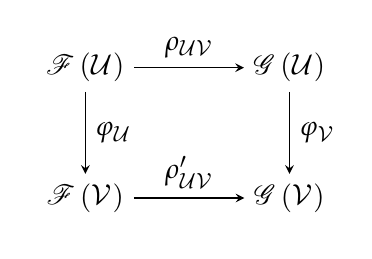
\begin{tikzpicture}
			\matrix (m) [matrix of math nodes,row sep=3em,column sep=4em,minimum width=2em]
			{
				\mathscr F\left( \sU\right)   & \mathscr G\left( \sU\right)\\
				\mathscr F\left( \sV\right)    & \mathscr G\left( \sV\right)\\
			};
			\path[-stealth]
			(m-1-1) edge node [above] {$\rho_{\sU\sV}$} (m-1-2)
			(m-1-1) edge node [right] {$\varphi_\sU$} (m-2-1)
			(m-1-2) edge node [right] {$\varphi_\sV$} (m-2-2)
			(m-2-1) edge node [above] {$\rho'_{\sU\sV}$} (m-2-2);
		\end{tikzpicture}
		\\
		is commutative, where $\rho_{\sU\sV}$ and $\rho'_{\sU\sV}$ are the restriction maps in $\mathscr F$  and $\mathscr G$. If $\mathscr F$  and $\mathscr G$ are sheaves on $\sX$, we use the same definition for a morphism 
		of sheaves. An isomorphism is a morphism  which has a two-sided inverse. 
	\end{definition}
	\begin{empt}\label{open_sheaf_empt}
		For any topological space $\sX$ there is a \textit{sheaf of stalks of open sets} $\Om_\sX$ on $\sX$ (cf. \cite{goldblatt:topoi})
		such that
		\bean
		\Om_\sX \left(\sU \right)  \bydef  \text{the family of all open subsets of }\sU;\\
		\rho_{\sU \sV}: \Om_\sX\left(\sU \right) \to \Om_\sX\left(\sV \right), \quad \mathcal W \mapsto \mathcal W \cap \sV.
		\eean
	\end{empt}
	
	\subsection{Cohomology}
	\paragraph{}
	The described below theories are specializations of described in sections \ref{grothendieck_cohomology_section} and \ref{presheaf_cohomology_sec} ones (cf. Example \ref{top_gro_exm}).
	%\begin{lemma}\cite{hartshorne:ag}
	%	Let $\sX$ be a topological space, and $\mathscr U$ an open covering of $\sX$. Then for any sheaf $\mathscr U$ on $\sX$ and	for each $r \ge 0$ there is a natural map, functorial in $\mathscr F$.
	%	$$
	%	\check{H}^r\left(\mathscr U, \mathscr F \right) \to H^r\left( \sX, \mathscr F\right) 
	%	$$
	%	where both $\check{H}^r$ and $H^r$ are given by the equations \eqref{cech_coh_eqn} and \eqref{etale_coh_eqn} respectively.
	%\end{lemma}
	%\begin{remark}
	%From the above lemma and the equation  \ref{chech_eqn} for each $r\ge 0$ one has a homomorphism
	%$$
	%\check{H}^r\left(\sX, \mathscr F \right) \to H^r\left( \sX, \mathscr F\right).
	%$$
	%\end{remark}
	\begin{empt}
		If $f: \sX\to\sY$ is a continuous map  $\mathscr U = \left\{\sU_\iota\right\}_{\iota} \in I$ is a covering of $\sY$ (cf. Definition \ref{pretopology_defn}   !!! NO SITE !!! and Example \ref{top_gro_exm}) then a family $f^{-1}\left(\mathscr U \right) \bydef \left\{f^{-1}\left( \sU_\iota\right) \right\}_{\iota} \in I$ is a covering of $\sX$. Let $F$ be a Abelian group, and let $F_\sX$, $F_\sY$ be a corresponding constant presheaves (cf. Definition \ref{constant_presheaf_defn}) on $\sX$ and $\sY$.  Following equation
		\be\label{top_cech_eqn}
		C^r\left( \mathscr U,  F_\sY\right)\bydef \prod_{\left(\iota_0,.... \iota_r\right) \in I^{r+1}}  F_\sY\left(\sU_{\iota_0,.... \iota_r} \right)\quad \text{where} \quad \sU_{\iota_0,.... \iota_r} \bydef \sU_{\iota_0}\cap...\cap \sU_{\iota_r}. 
		\ee
		is a specialization of \eqref{cech_eqn} one (cf. Example \ref{top_gro_exm}). For any $\left(\iota_0,.... \iota_r\right) \in I^{r+1}$ one has an isomorphism
		$$
		F_\sY\left(\sU_{\iota_0,.... \iota_r} \right)\cong F_\sX\left(f^{-1}\left( \sU_{\iota_0,.... \iota_r} \right)\right) \cong F.
		$$
		Above isomorphisms yield an isomorphism
		$$
		C^r\left( \mathscr U, F_\sY\right)\xrightarrow{\approx} C^r\left( f^{-1}\left( \mathscr U\right) , F_\sX\right)
		$$
		So there is an isomorphism
		$$
		\varinjlim_{\mathscr U}\check{H}^r\left( \mathscr U, F_\sY\right)\xrightarrow{\approx}\varinjlim_{\mathscr U}\check{H}^r\left(f^{-1}\left(  \mathscr U\right) , F_\sX\right).
		$$
		On the other hand from   \eqref{chech_eqn}  it follows that there are homomorphisms
		\bean
		\check{H}^r\left(f^{-1}\left(  \mathscr U\right) , F_\sX\right)\to \check{H}^r\left(\sX , F_\sX\right),\\
		\varinjlim_{\mathscr U} \check{H}^r\left(f^{-1}\left(  \mathscr U\right), F_\sX\right)\to \check{H}^r\left(\sX , F_\sX\right)
		\eean
		so one has a homomorphism
		$$
		\varinjlim_{\mathscr U} \check{H}^r\left(  \mathscr U, F_\sY\right)\to \check{H}^r\left(\sX , F_\sX\right)
		$$
		and applying \eqref{chech_eqn} one can obtain a natural homomorphism
		$$
		\check{H}^r\left(f\right):\check{H}^r\left(\sY, F_\sY \right)\to \check{H}^r\left(\sX, F_\sX \right)\quad r \ge 0.
		$$
		The details of the construction of the homomorphism $\check{H}^r\left(f\right)$  are explained in \cite{eust}. Using the Notation \ref{constant_presheaf_defn} one has homomorphisms
		\be\label{cech_hom_eqn}
		\begin{split}
			\check{H}^r\left(f\right):\check{H}^r\left(\sY, F \right)\to \check{H}^r\left(\sX, F \right)\quad r \ge 0,\\
			\check{H}^\bullet\left(f\right):\check{H}^\bullet\left(\sY, F \right)\to \check{H}^\bullet\left(\sX, F \right).
		\end{split}
		\ee
		If both $\sX \xrightarrow{f}\sY$ and $\sY \xrightarrow{g}\sZ$ are continuous maps then from this construction it turns out that
		\be\label{cech_hom_comp_eqn}
		\begin{split}
			\check{H}^\bullet\left(g\circ f\right)= \check{H}^\bullet\left( f\right)\circ \check{H}^\bullet\left(g\right):\check{H}^\bullet\left(\sZ, F \right)\to \check{H}^\bullet\left(\sX, F \right)
		\end{split}
		\ee
		
	\end{empt}
	
	\begin{empt}\label{tens_prop_c_empt}\cite{bryl:loop}
		\v{C}ech cohomology has the advantage of allowing an easy and explicit construction of a \textit{cup}-\textit{product}
		$$
		\check{H}^p\left(\mathscr U,  \mathscr F\right) \otimes \check{H}^q\left(\mathscr U,  \mathscr G\right)\to \check{H}^p\left(\mathscr U,  \mathscr F\otimes \mathscr G\right).
		$$
		Here $\mathscr F$ and $\mathscr G$ are sheaves of Abelian groups on $\sX$, and the \textit{tensor product}-\textit{sheaf}
		$\mathscr F\otimes \mathscr G$ is the sheaf associated to the presheaf $\sU \mapsto \mathscr F(\sU)\otimes \mathscr G(\sU)$. The 
		stalk (cf. Definition \ref{stalk_defn}) at $x$ of $\mathscr F\otimes \mathscr G$ is $\mathscr F_x\otimes \mathscr G_x$. The cup-product will be defined from a 
		morphism of complexes. We first need the notion of tensor product $A^\bullet \otimes  B^\bullet$
		of two complexes; this is the total complex of the double complex $A^\bullet \otimes  B^\bullet$. 
		So the degree $n$-term of $A^\bullet \otimes  B^\bullet$ is $\oplus A^p\otimes B^{n-p}$. The differential in $A^\bullet \otimes  B^\bullet$  
		is 
		$$
		d \left(a \otimes b\right)	\bydef \left(da\right)\otimes b + \left(-1\right)^p a \otimes db
		$$
		
		for $a\in A^p$, $b \in B^q$. We have the obvious 
		map 
		$$
		\otimes :H^p\left(A^\bullet\right)\otimes H^q\left(B^\bullet\right)\to H^q\left(A^\bullet\ox B^\bullet\right).	
		$$	
		We now return to the sheaves $\mathscr F$ and $\mathscr G$ of Abelian groups on $\sX$. We 
		have the complexes $C^\bullet\left(\mathscr U,  \mathscr F\right)$ and $C^\bullet\left(\mathscr U,  \mathscr G\right)$.  The interesting part is the 
		construction of a morphism of complexes 
		$$
		\phi: C^\bullet\left(\mathscr U,  \mathscr F\right)\otimes C^\bullet\left(\mathscr U,  \mathscr G\right)\mapsto C^\bullet\left(\mathscr U,  \mathscr F\otimes  \mathscr G\right).
		$$
		For $\a \in C^\bullet\left(\mathscr U,  \mathscr F\right)$ and $\bt \in C^\bullet\left(\mathscr U,  \mathscr G\right)$, we put 
		$$
		\phi:\left( \a \otimes \bt \right)_{\iota_0,..., \iota_{p + q}} \bydef \a_{\iota_0,...,\iota_p}\otimes  \bt_{\iota_{p},..., \iota_{p+q}}.
		$$
		One checks easily that $\phi$ is indeed a morphism of complexes. The induced map on cohomology gives the cup-product on \v{C}ech 
		cohomology. For $\a$ degree $p$ \v{C}ech cocycle with coefficients in $\mathscr F$ and $\bt$
		degree $q$ \v{C}ech cocycle with coefficients in $\mathscr G$, we have 
		\be\label{cup_prod_eqn}
		\left(\a \smile\bt \right)_{\iota_0,..., \iota_{p + q}}\bydef  \a_{\iota_0,...,\iota_p}\otimes  \bt_{\iota_{p},..., \iota_{p+q}}.
	\ee
		The cup-product has the following properties. 
	\end{empt}
	\begin{proposition}\label{cup_ass_prop}\cite{bryl:loop} Following conditions hold.
		%	1.3.7. Proposition. 
		\begin{enumerate}
			\item[(i)] The cup-product is associative, i.e., for $\a \in \check{H}^p\left(\mathscr U,  \mathscr F\right)$,  $\bt \in \check{H}^q\left(\mathscr U,  \mathscr G\right)$, $\ga \in \check{H}^r\left(\mathscr U,  \mathscr H\right)$
			we have 
			$$
			\a \smile \left( \bt \smile \ga\right) 	= \left( \a \smile \bt\right) \smile \ga. 
			$$
			\item[(ii)]	 The \textit{cup}-\textit{product} is \textit{graded}-\textit{commutative}. If $\a \in \check{H}^p\left(\mathscr U,  \mathscr F\right)$,  $\bt \in \check{H}^q\left(\mathscr U,  \mathscr G\right)$, we have 
			$$
			\a \smile \bt =\left( -1\right)^p  \bt \smile \a.
			$$			
			
		\end{enumerate}
		
	\end{proposition}
	\begin{empt}
		Let $\sX$ be a topological space. If $R$ be an ring then there is, a corresponding constant presheaf  $R_\sX$ (cf. Definition \ref{constant_presheaf_defn}) on $\sX$. 
		Using the cup product and homomorphism $\phi$ one has a map
		$$
		\check{H}^\bullet\left(\sX, R_\sX \right)\times \check{H}^\bullet\left(\sX, R_\sX \right) \to \check{H}^\bullet\left(\sX, R_\sX \right).
		$$
		So we have proved the following.	
	\end{empt}
	
	\begin{lem}\label{gr_ring_lem}
		Let $\sX$ be a topological space. If $F$ is an Abelian group then any isomorphism $F \otimes_\Z F \cong  F$ yields a product
		\bean
		\smile: \check{H}^\bullet\left(\sX, F \right)\otimes \check{H}^\bullet\left(\sX,F \right) \to \check{H}^\bullet\left(\sX,F \right)
		\eean
		where the notation \eqref{etale_hom_a_eqn} is used. So $\check{H}^\bullet\left(\sX, F\right)$ becomes an associative and graded-commutative ring.
	\end{lem}
	
	\begin{exercise}\label{ring_homo_exer}
Prove that a given by \eqref{cech_hom_eqn} map $\check{H}^\bullet\left(f\right):\check{H}^\bullet\left(\sY, F \right)\to \check{H}^\bullet\left(\sX, F \right)$ is a homomorphism of rings.
	\end{exercise}
	
	\begin{remark}\label{ring_homo_rem}
	In \cite{milne:lec,swan:cup} it is explained that the Lemma \ref{gr_ring_lem} and the Exercise  \ref{ring_homo_exer} can by applied to any Grothendieck topology.
	\end{remark}
	
	\section{$C^*$-algebras}
	\paragraph*{}  
	A notion of $C^*$-algebra is explained in \cite{murphy, pedersen:ca_aut, rae:ctr_morita}.
	
	\begin{thm}(Dauns Hofmann)\label{dauns_hofmann_thm}\cite{pedersen:ca_aut}
		For each $C^*$-algebra $A$ there is the natural isomorphism from the center of $M\left( A\right)$ onto the class of bounded continuous  functions on $\check{A}$. 
	\end{thm}
	
%	\begin{definition}\label{atomic_repr_defn}\cite{pedersen:ca_aut}
%		Let $A$ be a $C^*$-algebra with the spectrum $\hat A$. We choose for any $t \in \hat A$ a pure state $\phi_t$ and  associated representation $\pi_t: A \to B\left(\H_t\right)$.		The representation 
%		\be
%		\pi_a = \bigoplus_{t \in \hat A} \pi_t \quad \text{on the closure } \H_a \text{ of an algebraic direct sum}\quad  \bigoplus_{t \in \hat A} \H_t
%		\ee
%		is called the (reduced) \textit{atomic representation} of $A$. Any two atomic representations are unitary equivalent and any atomic representation of $A$ is faithful and nondegenerate  %(cf.  Definitions \ref{faithful_repr_defn}, \ref{nondegenerate_repr_defn} and \cite{pedersen:ca_aut}).
%	\end{definition}
	

	\begin{definition}\label{lrc_defn}\cite{matro:hcm}
	If $A$ is a $C^*$-algebra then a linear map $\la: A\to A$ is said to be a \textit{left centralizer} if
	\be
	\la\left(ab\right)= 	\la\left(a\right) b \quad \forall a, b \in A.
	\ee
	Similarly one defines a \textit{right} centralizer. Denote the spaces of left and right centralizers by $\mathbf{LC}(A)$ and  $\mathbf{RC}(A)$.
	\end{definition}
	
		
%	\begin{definition}\label{qc_defn}\cite{matro:hcm}
%A linear map $q: A\times A \to A$ is called a \textit{quasi}-\textit{centralizer} if
%\bean
%\la_a \in \mathbf{LC}(A), \quad \text{where}\quad  \la_a : \quad b \mapsto q\left(a, b \right) \quad \forall a, b \in A,\\
%\rho_b \in \mathbf{RC}(A), \quad \text{where}\quad  \rho_b : \quad a \mapsto q\left(a, b \right) \quad \forall a, b \in A.\\
%\eean 
%In other words,
%\bean
%q\left(ca, bd\right)= cq\left(a, b\right)d \quad \forall a, b, c, d \in A 
%\eean 
% Denote the space of quasi-centralizers by $\mathbf{QC}(A)$.
%	\end{definition}
	
	\begin{lem}
	If $\rho\in  \mathbf{RC}(A)$ then $\rho^*\in  \mathbf{LC}(A)$ where $\rho^*\left(a \right)\bydef \left(\rho\left( a^* \right) \right)^*$. 
	\end{lem}
	
	\begin{empt}\label{gen_rel_empt}
		The notion of \textit{generators and relations} $\left(G, R\right)$ is explained in \cite{phillips:inv_lim_app}. There is the   \textit{universal $C^*$-algebra on the generators $G$ and relations $R$} (cf. \cite{phillips:inv_lim_app} for details). We denote it by $C^*\left(G, R\right)$.
	\end{empt}
	
	\subsection{Hereditary $C^*$-subalgebras}
	
	\begin{definition}\label{hered_defn}\cite{pedersen:ca_aut}
		A cone $M$ in the positive part of $C^*$-algebra $A$ is said to be \textit{hereditary} if $0 \le x \le y$, $y \in M$ implies $x \in M$ for each $x \in A$. A $C^*$-subalgebra $B$ of $A$ is \textit{hereditary} if $B_+$ is hereditary in $A_+$.
	\end{definition}
	%\begin{lemma}\label{hered_lem}\cite{murphy}
	%	Let $B$ be a $C^*$-subalgebra of $C^*$-algebra $A$. Then $B$ is hereditary in $A$ if and only if $bab' \in B$ for all $b, b' \in B$ and $a \in A$.
	%\end{lemma}
	\begin{lemma}\label{hered_ideal_lem}\cite{murphy}
		Let $A$ be a $C^*$-algebra.
		\begin{enumerate}
			\item[(i)] If $L$ is a closed left ideal in $A$ then $L\cap L^*$ is a hereditary $C^*$-subalgebra of $A$. The map $L \mapsto L\cap L^*$ is the bijection from the set of closed left ideals of $A$ onto the the set of hereditary $C^*$-subalgebras of $A$.
			\item[(ii)] If $L_1, L_2$ are closed left ideals, then $L_1 \subseteq L_2$ is and only if $L_1\cap L_1^* \subset L_2\cap L_2^*$.
			\item[(iii)] If $B$ is a hereditary $C^*$-subalgebra of $A$, then the set 
			\be\label{left_ideal_eqn}
			L\left(B \right) = \left\{\left.a \in A~\right| a^*a \in B\right\}
			\ee
			is the unique closed left ideal of $A$ corresponding to $B$.
		\end{enumerate}
	\end{lemma}
	
	
	\begin{remark}\label{hered_rem}\cite{murphy}
		Obviously, $0$ and
		$A$ are hereditary $C^*$-subalgebras of $A$, and any intersection of hereditary
		$C^*$-subalgebras is one also. 
		
	\end{remark}
	\begin{definition}\label{hered_generated_defn}\cite{murphy}
		The hereditary $C^*$-subalgebra \textit{generated} by a
		subset $S$ of $A$ is the smallest hereditary $C^*$-subalgebra of $A$ containing $S$.
	\end{definition}
	
	
	\begin{lemma}\label{hered_repr_lem}\cite{pedersen:ca_aut}
		%4.1.5. LEMMA. 
		Let $B$ be a hereditary $C^*$-subalgebra of $A$. For each irreducible 
		representation $\pi: A \to B\left( \H\right)$  such that $B \not\subset\ker\pi$ the map $\pi|_B: B \to \pi\left(B \right)\H$  is an irreducible 
		representation of $B$. 
		
	\end{lemma}
	\begin{defn}\label{approximate_unit_defn} \cite{pedersen:ca_aut}
		Let $A$ be a $C^*$-algebra. A net $\left\{u_\la \right\}_{\la \in \La}$ in $A_+$ with $\left\|u_\la \right\| \le 1$ for all $\la \in \La$ is called an \textit{approximate unit} for $A$ if $\la < \mu$ implies $u_\la < u_\mu$ and if $\lim \left\|x- xu_\la \right\| = 0$ for each $x$ in $A$. Then, of course, $\lim \left\|x- u_\la x \right\| = 0$ as well.
	\end{defn}
		\begin{thm}\label{approximate_unit_thm} \cite{pedersen:ca_aut}
		Each $C^*$-algebra contains an \textit{approximate unit}.
	\end{thm}
	
	
	\begin{theorem}\label{left_ideal_thm}\cite{murphy}
		%3.1.2. Theorem.
		If $L$ is a closed left ideal in a $C^*$-algebra $A$, then there
		is an increasing net $\left\{u_\la\right\}_{\la\in\La}$ of positive elements in the closed unit ball of
		$L$ such that $a = \lim_{\la\in \La}au_\la $ for all $a\in L$.
	\end{theorem}
	\subsection{Topologies of $C^*$-subalgebras}
	
	\begin{defn}\label{strict_topology_defn}\cite{pedersen:ca_aut}
		Let $A$ be a $C^*$-algebra.  The {\it strict topology} on the multiplier algebra $M(A)$ is the topology generated by seminorms 
		\be\label{strict_topology_norm_eqn}
		\vertiii{x}_a\bydef \|ax\| + \|xa\|,\quad a\in A.
		\ee
		If $\La$ is a directed set and $\left\{a_\la\in M\left( A\right) \right\}_{\la\in \La}$ is a net the we denote by $\bt\text{-}\lim_{\la\in\La }a_\la$ the limit of $\left\{a_\la \right\}$ with respect to the strict topology.
	\end{defn}
	
	
	\begin{defn}\label{commutant_defn}
		%2.2.1. 
		For each subset $M$ of $B(\H)$ let $M'$ denote the \textit{commutant} of $M$, i.e. 
		\bean
		M'\bydef \left\{b \in B\left(\sH\right)|\forall a \in M \quad ab = ba \right\}
		\eean
		The $C^*$-algebra 
		\bean
		M''\bydef (M')'
		\eean
		is said to be a \textit{bicommutant} of $M$.
	\end{defn}
		\begin{defn}
		\label{strong_topology_defn}\cite{pedersen:ca_aut} Let $\H$ be a Hilbert space. The {\it strong} topology on $B\left(\H\right)$ is the locally convex vector space topology associated with the family of seminorms of the form $x \mapsto \|x\xi\|$, $x \in B(\H)$, $\xi \in \H$.
	\end{defn}
	\begin{thm}\label{von_Neumann_thm}\cite{pedersen:ca_aut}
		Let $M$ be a $C^*$-subalgebra of $B(\H)$, containing the identity operator. The following conditions are equivalent:
		\begin{itemize}
			\item $M=M''$ where $M''$ is the bicommutant of $M$;
			\item $M$ is weakly closed;
			\item $M$ is strongly closed.
		\end{itemize}
	\end{thm}
	\begin{lemma}\label{increasing_convergent_w_lem}\cite{pedersen:ca_aut} Let $\Lambda$ be an increasing in the partial ordering.  Let $\left\{x_\lambda \right\}_{\la \in \La}$ be an increasing of self-adjoint operators in $B\left(\H\right)$, i.e. $\la \le \mu$ implies $x_\la \le x_\mu$. If $\left\|x_\la\right\| \le \ga$ for some $\ga \in \mathbb{R}$ and all $\la$ then $\left\{x_\lambda \right\}$ is strongly convergent to a self-adjoint element $x \in B\left(\H\right)$ with $\left\|x_\la\right\| \le \ga$.
\end{lemma}
	

	

	
	
	
	
	
	\subsection{$C^*$-algebras of type I}
	
	\begin{definition}\label{type_i0_defn}\cite{pedersen:ca_aut}
		% 6.1
		A positive element $a$ in a $C^*$-algebra $A$ is \textit{Abelian} if 
		the hereditary $C^*$-subalgebra generated by $a$, i.e. the norm closure of $aAa$, is 
		commutative. If $A$ is  generated (as a $C^*$-algebra) 
		by its Abelian elements we say that it is of \textit{type} $I_0$. We say that a C*-algebra A is of \textit{type} $I$ if each non-zero quotient of A 
		contains a non-zero Abelian element.
	\end{definition}
	\begin{lemma}\label{type_i0_lem}\cite{pedersen:ca_aut}
		%6.1.3. LEMMA 
		A positive element $a$ in a $C^*$-algebra $A$ is Abelian if and only if $\dim \pi\left(a \right)\le 1$ for every irreducible representation $\pi: A \to B\left(\H \right)$. 
	\end{lemma}	
	%\begin{definition}\cite{pedersen:ca_aut}
%	By a \textit{composition series} for a $C^*$-algebra $A$ we mean a strictly increasing 	family of closed ideals $\left\{I_\a\right\}$ indexed by a segment $\left\{0\le \a\le \bt\right\}$ of the ordinals 	such that $I_0 = \{0\}$, $I_\bt = A$; and for each limit ordinal y we have 
%	$$
%	I_\ga = \left(\bigcup_{\a < \ga}\right)^- \quad \text{norm closure}
%	$$
%%	If each $I_\a$ is an essential ideal in $I_{\a+1}$ we say that the composition series is 	essential. It is clear that a composition series for a separable C*-algebra can be 	at most countable. 
%	\end{definition}
%	\begin{theorem}\label{comp_thm}\cite{pedersen:ca_aut}
%	The following conditions on a C*-algebra A are equivalent: 
%	\begin{enumerate}
%		\item[ 	(i)] $A$ is of type $I$; 
%		\item[(ii)] $A$ has a composition series $\left\{I_\a| 0 \le \a \le \bt\right\}$ such that $I_{\a + 1}/ I_\a$ is of type $I_0$
%		for each $\a < \bt$; 
%	\end{enumerate}
%	\end{theorem}
	\begin{definition}\label{continuous_trace_c_alt_defn}\cite{rae:ctr_morita}
		%Definition 5.13. 
		A \textit{continuous-trace} $C^*$-\textit{algebra} is a $C^*$-algebra $A$ with Hausdorff
		spectrum $\sX$ such that, for each $x_0\in\sX$ there are a neighborhood $\sU$ of $x_0$ and $a\in A$ such that $\rho_{ x}\left( a\right) $ is a rank-one projection for all $x \in \sU$, where $\rho_{ x}: A \to B\left(\H_x\right)$ is a corresponding to $x$ irreducible representation.
	\end{definition}
	\begin{remark}\label{ctr_gen_rem}\cite{pedersen:ca_aut}
		Any {continuous-trace} $C^*$-{algebra}  $A$ is of type $I_0$.
	\end{remark}
	
	\begin{lemma}\label{ctr_rep_eq_lem}\cite{rae:ctr_morita}
		Suppose $A$ is a $C^*$-algebra with Hausdorff spectrum $\mathcal{X}$ and for all $x \in \sX$ $\pi_x : A \to B\left(\H_x \right)$ is a corresponding  to $x$ irreducible representation then for each $a \in A$ the function $x \mapsto \left\|\pi_x\left(a \right) \right\|$ is continuous on  $\mathcal{X}$, vanishes at infinity and has sup-norm equal to $\left\| a\right\|$. 
	\end{lemma}
	\begin{rem}\label{ctr_spe_rem}
		From the Lemma \ref{hered_repr_lem} it follows that if $A$ 	 has continuous trace and $\sX$ is a spectrum of $A$ then a spectrum $\sX_B$ of any hereditary subalgebra $B$ is an open subset of $\sX$ (cf.  \cite{pedersen:ca_aut} for details).
	\end{rem}
	
		\subsection{ Dixmier-Douady duality}\label{dd_dual_sec}
	\begin{proposition}\label{ctr_lt_prop}\cite{cuntz_meyer_ros:bivariant}
		%Proposition 9.3. 
		Let $\H$ be a Hilbert space, and let $\K \bydef \K\left(\H \right)$  be the algebra of
		compact operators on $\H$. Then every irreducible *-representation of $\K$ is unitary
		equivalent to the standard representation of $\K$ on $\sH$, and every $*$-automorphism
		of $\K$ is given by conjugation by a unitary operator on $\H$. The *-automorphism
		group of $\K$ can be identified with the topological group $PU\bydef U/\T$ the
		projective unitary group of $\H$, with the quotient topology from the strong operator
		topology on $U\left(\H\right)$.
	\end{proposition}
	
	\begin{proposition}\label{ctr_bundle_prop}\cite{cuntz_meyer_ros:bivariant}
		%Proposition 5.59. 
		%Theorem 9.9 
		(Dixmier�Douady). 
		Any stable separable algebra A of continuous
		trace over a second-countable locally compact Hausdorff space $\sX$ is isomorphic to
		$\Ga_0\left( \sX, \sF\right)$ , the sections vanishing at infinity of a locally trivial bundle of algebras
		over $\sX$, with fibres $\K$ and structure group $\Aut(\K) = PU = U/\T$. Classes of
		such bundles are in natural bijection with the \v{C}ech cohomology group $\check{H}^3\left(\sX, \Z \right)$.
		The 3-cohomology class $\dl\left( A\right)$  attached to (the stabilization of) a continuous-trace
		algebra A is called its Dixmier�Douady class.
	\end{proposition}
	\begin{proof}
		Principal $PU$-bundles over $\sU$ are thus classified by
		$\left[\sX, BPU\right] = \left[\sX, K\left( \Z, 3\right) \right] = H^3\left(\sX, \Z \right)$. 
		The details of the proof are presented in \cite{cuntz_meyer_ros:bivariant}.
	\end{proof}
	
	\begin{proposition}\label{ctr_d_prop}\cite{cuntz_meyer_ros:bivariant}
		%Proposition 9.11 (P. Green [51,96,104]). 
		Let $\sX$ be a second-countable locally compact
		Hausdorff space, and let $A$ and $B$ be stable algebras of continuous trace over $\sX$.
		Then $A \times_\sX B$ is also a stable continuous-trace algebra over $\sX$, and the Dixmier�Douady class $\dl \left(A \otimes_\sX B \right)$  of $A \times_\sX B$ is given by $\dl(A) + \dl(B)$. The Dixmier�Douady class of the opposite algebra $A^{\mathrm{op}}$ is given by $\dl\left( A^{\mathrm{op}}\right)=$ - $\dl\left( A\right)$ , so that
		$A\times_\sX  A^{\mathrm{op}}= C_0\left(\sX, \K\right)$.
	\end{proposition}
	\begin{notation}\label{ctr_not}
		If $\sX$ is a locally compact Hausdorff space then we denote by $CT\left(\sX, \dl \right)$ the stable
		continuous-trace algebra  with Dixmier�Douady class $\delta \in \check{H}^3\left(\sX,\Z \right)$. From the Proposition \ref{ctr_d_prop} it follows that
		\be\label{bundle_prod_iso}
		\varphi_{\dl \rho}	:CT\left(\sX, \dl \right)\times_\sX CT\left(\sX, \rho \right)\cong CT\left(\sX, \dl +\rho\right).
		\ee
	\end{notation}
	\begin{proposition}\label{ctr_cup_prop}\cite{cuntz_meyer_ros:bivariant}
		%Proposition 9.17.
		There are natural homomorphisms
		\bea\label{ka_eqn}
		K_\bullet\left( CT\left(\sX, \dl \right)\right)\otimes_\Z K_\bullet\left( CT\left(\sX, \rho \right)\right) \to K_\bullet\left( CT\left(\sX, \dl + \rho\right)\right),\\
		\label{kx_eqn}
		K_\bullet\left( CT\left(\sX, 0 \right)\right)\cong K^\bullet\left( \sX\right),
		\eea
		where $K_\bullet\left( CT\left(\sX, \dl \right)\right)$ means $K$-theoretic groups of $C^*$-algebra $ CT\left(\sX, \dl \right)$ and $K^\bullet\left( \sX\right)$ means $K$-theoretic groups of the space $\sX$.
	\end{proposition}
	\subsection{Cuntz algebras}\label{cuntz_alg_sec}
	\paragraph{} Here I follow to \cite{cuntz_alg}.
	We consider the $C^*$-algebra $\mathcal O_n$ generated by $n \ge 2$ isometries $S_1, ..., S_n$
	on an infinite-dimensional Hubert space, with the property that $S_1S^*_1 + ... + S_nS^*_n = 1_{\mathcal O_n}$. Given $n\in \N$, let $W^n_k$ be the set of all $k$-tuples $\left(j_1,..., j_k\right)$, with $j_l \in \left\{1, ..., n\right\}$. Let $W^n_0 \bydef 0$ and 
\be\label{words_eqn}	
W^n_\infty \bydef \bigcup_{k = 0}^\infty W^n_k
\ee
For any $\a =  \left(j_1,..., j_k\right) \in W^n_k\subset W^n_\infty$ denote by
\be\label{words_a_eqn}
\begin{split}
S_\a \bydef S_{j_1} \cdot ...\cdot S_{j_k}.
\end{split}	
\ee
\begin{statement}\label{word_stmt}\cite{cuntz_alg}
The $C^*$-algebra $\mathcal O_n$ is the $C^*$-norm completion of the linear span of given by 
\bean
S_\mu S^*_\nu \quad \mu, \nu \in W^n_\infty 
\eean
\end{statement}
It is proven in \cite{cuntz_alg} that
\be\label{ss_eqn}
S^*_\mu S_\nu  = \dl_{\mu\nu} 1_{\mathcal O_n}.
\ee


	\section{Groupoids, foliations,  and $C^*$-algebras}\label{foliations_sec}
	\subsection{Groupoids and their $C^*$-algebras}
	\paragraph*{}
	A groupoid is a small category with inverses, or more explicitly:
	\begin{definition}\label{groupoid_defn}\cite{renault:gropoid_ca}
		% 104
		A \textit{groupoid} consists of a set $\G$, a distinguished subset $\G^0\subset\G$, two maps
		$r, s : \G\to \G^0$ and a law of composition
		$$
		\circ: \G^2\bydef\left\{\left.\left(\ga_1,\ga_2 \right) \in \G\times\G~\right| s\left(\ga_1\right)= r\left(\ga_2\right)\right\}\to \G
		$$
		such that
		\begin{enumerate}
			\item $s\left(\ga_1\circ\ga_2\right)=s\left(\ga_2\right), \quad r\left(\ga_1\circ\ga_2\right)=r\left(\ga_1\right)\quad \forall\left(\ga_1, \ga_2 \right) \in \G$
			\item $s\left(x\right)=r\left(x\right)=x \quad\forall x\in\G^0$
			\item $\ga\circ s\left(\ga\right)= r\left(\ga\right)\circ\ga = \ga\quad \forall\ga\in\G$
			\item $\left( \ga_1\circ\ga_2\right) \circ\ga_3=\ga_1\circ\left( \ga_2\circ\ga_3\right) $
			\item Each $\ga \in\G$ has a two-sided inverse $\ga^{-1}$, with $\ga\circ\ga^{-1}=r\left(\ga\right)$, $\ga^{-1}\circ\ga=r\left(\ga\right)$.
		\end{enumerate}
		The maps $r$, $s$ are called the \textit{range} and \textit{source} maps.
	\end{definition}
	
	\begin{empt}\label{cycle_empt}\cite{renault:gropoid_ca}
		The notion of \textit{topological groupoid} is explained in \cite{renault:gropoid_ca}. 
		If $F$ is an Abelian group then then for all $r \ge 0$ there is $r^{\text{th}}$ \textit{cohomology group} $H^r\left( \G, F\right)$. Any element of $H^2\left( \G, F\right)$ can be represented  by a 2-\text{cycle} $\a \in Z^2\left(\G, F \right)$. Note that a 2-cycle $\a$ is a map   $\G^2 \to F$. If $\G$ is a topological groupoid and  $F$ is a topological group then we assume that the map $\a$ is continuous. We write $\left[\a\right]\in H^r\left( \G, F\right)$.
	\end{empt}
	\begin{remark}\label{hoto_rem}
		If both $\a', \a''\in \Z^2\left(\G, F \right)$ are homotopic 2-cocycles  then  $\left[\a'\right]= \left[\a''\right]\in H^2\left( \G, F\right)$.
	\end{remark}
	\begin{empt}\label{groupoid_haar_empt}\cite{renault:gropoid_ca}
		The notion of  \textit{left Haar system} on locally compact groupoid is explained in \cite{renault:gropoid_ca}. Let $\G$ be a locally compact groupoid with left Haar system $\left\{\la^u\right\}$ and let $\a$ be a continuous 2-cocycle in $Z^2\left(\G, \T\right)$. For $f ,g \in C_c(\G )$, let us define
		\bea\label{groupoid_*_c_eqn}
		f * g \left(x\right)\bydef 
		\int f ( x y ) g \left( y^{-1}\right)\a\left(xy, y^{-1} \right) d\la^{d(x)}(y),\\
		\label{groupoid_inv_c_eqn}
		f^* ( x ) \bydef \overline{f ( x^{ -1})}~\overline{\a\left(x, x^{-1} \right)}, 	
		\eea
		so $ C_c(\G )$ becomes a *-algebra, we denote it by $C_c\left( \G, \a\right)$. Denote by $C^*_r\left( \G, \a\right)$ a completion of  $C_c\left(\G, \a\right)$ with respect to the following $C^*$-norm
		\be\label{groupoid_norm_eqn}
		\left\|a \right\| \bydef \sup_{\pi \in \text{Irr}\left(C_c\left(\G\right)\right)} \left\|\pi\left( a\right)  \right\| 
		\ee
		where $\text{Irr}\left(C_c\left(\G\right)\right)$ is a set of all irreducible representations of $C_c\left(\G\right)$.
	\end{empt}
	\begin{proposition}\label{cohom_groupoid_prop}\cite{renault:gropoid_ca}
		%1.2. Proposition : 
		If $\a$ and $\a'$ are cohomologous, then $C_c\left( \G, \a\right)$  and $C_c\left( \G, \a'\right)$ are
		isomorphic.
	\end{proposition}
	\begin{statement}\label{gropoid_mult_lem}\cite{renault:gropoid_ca}
If $C^*_r\left( \G, \a\right)$ is a completion of $C_c\left( \G, \a\right)$ with respect to the norm \eqref{groupoid_norm_eqn}, then there is the natural inclusion $C_0\left(\G^0 \right) \hookto M\left( C^*_r\left( \G, \a\right)\right)$.
	\end{statement}
	
	\subsection{Foliations}
	\begin{definition}\label{foli_rect_defn}\cite{candel:foliI}	% 	Definition 1.1.16 \\
		A rectangular neighborhood in $\mathbb{F}^n$ is an open subset of the form $B = J_1\times...\times J_n$, where each $J_j$ is a (possibly unbounded) relatively open interval in the $j^{\text{th}}$ coordinate axis. If $J_1$ is of the form $\left( a,0\right]$, we say that $B$ has boundary $\partial B\left\{\left(0, x_2,..., x_n \right)\right\}\subset B$.	%In the following, we will consider coordinate charts that have values in F" x F", allowing the possibility of manifolds with boundary and (convex) COI'Ile1'S.
	\end{definition}
	\begin{definition}\label{foli_chart_defn}\cite{candel:foliI}
		% 	Definition 1.1.17 \\
		Let $M$ be an $n$-manifold. A \textit{foliated chart} on $M$ of codimension $q$ is a pair $\left(\sU, \varphi)\right)$, where $\sU\subset M$ is open and $\varphi : \sU \xrightarrow{\approx} B_\tau\times B_\pitchfork$ is a diffeomorphism, $B_\pitchfork$ being a rectangular neighborhood in $\mathbb{F}^q$ and $B_\tau$ a rectangular neighborhood in $\mathbb{F}^{n-q}$. The set $P_y = \varphi^{-1}\left(B_\tau \times \left\{y\right\} \right)$ , where $y \in B_\pitchfork$, is called a \textit{plaque} of this foliated chart. For each $x \in B_\tau$, the set  $S_x=\varphi^{-1}\left(\left\{x\right\} \times B_\pitchfork \right)$  is called a \textit{transversal} of the foliated chart. The set $\partial_{\tau}\sU = \varphi^{-1}\left(B_\tau \times \left(\partial B_\pitchfork \right)  \right)$ is called the \textit{tangential boundary} of $\sU$ and $\partial_{\pitchfork}\sU = \varphi^{-1}\left(\partial \left( B_\tau\right)  \times \partial B_\pitchfork \right)$ is called the \textit{transverse boundary} of $\sU$.
	\end{definition}
	
	
	\begin{definition}\label{foli_trans_defn}\cite{candel:foliI}
		Let $N \subset M$ be a smooth submanifold. We say that $\sF$ is \textit{transverse} to $N$ (and write $\sF\pitchfork N$) if, for each leaf $L$ of $\sF$ and each point $x \in L\cap N$, $T_x\left(L \right)$ ans $T_x\left(N \right)$ together span $T_x\left( M\right)$. At the other extreme At the other extreme, we say that $\sF$ is tangent to $N$ if, for each leaf $L$ of $\sF$, either $L \cap N = \emptyset$ or $L \subset N$.
	\end{definition}
	The symbol $\mathbb{F}^p$ denotes either the full Euclidean space $\R^p$ or Euclidean half space $\mathbb{H}^p = \left\{\left.\left(x_1,..., x_n \right) \in \mathbb{R}^p\right| x_1 \le 0 \right\}$.
	\begin{definition}\label{foli_manifold_defn}\cite{candel:foliI}
		% Definition 1.1.18
		Let $M$ be an $n$-manifold, possibly with boundary and corners, and let $\sF= \left\{L_\la\right\}_{\la \in \La}$ be a decomposition  of $M$ into connected, topologically immersed submanifolds of dimension $k=n-q$. Suppose that $M$ admits an atlas $\left\{\sU_\a \right\}_{\a \in \mathfrak A}$ of foliated charts of codimension $q$ such that, for each $\a \in \mathscr A$ and each $\la \in \La$, $L_\la \cap \sU_\a$ is a union of plaques. Then $\sF$ is said to be a \textit{foliation} of $M$ of codimension $q$ (and dimension $k$) and $\left\{\sU_\a \right\}_{\a \in \mathscr A}$  is called a \textit{foliated atlas} associated to $\sF$. Each $L_x$ is called a leaf of the foliation and the pair $\left(M, \sF \right)$  is called a \textit{foliated manifold}. If the foliated atlas is of class $C^r$ ($0 \le r \le \infty$ or $r=\om$), then the foliation $\sF$ and the foliated manifold $\left(M, \sF \right)$. is said to be \textit{of class} $C^r$.
	\end{definition}
	\begin{definition}\label{foli_atlas_defn}
		A \textit{foliated atlas} of codimension $q$ and class $C^r$ on the $n$-manifold $M$ is a $C^r$-atlas $\mathfrak{A}\bydef\left\{\sU_\a \right\}_{\a \in \mathscr A}$  of foliated charts of codimension $q$ which are \textit{coherently foliated} in the sense that, whenever $P$ and $Q$ are plaques in distinct charts of $\mathfrak{A}$, then $P\cap Q$ is open both in $P$ and $Q$. 
	\end{definition}
	\begin{definition}\label{foli_coh_atlas_defn}
		Two foliated atlases lt and $\mathfrak{A}$ on $\mathfrak{A}'$ of the same codimension and smoothness class $C^r$ are \textit{coherent} ($\mathfrak{A}\approx\mathfrak{A}'$) if $\mathfrak{A}\cup\mathfrak{A}'$ is a foliated $C^*$-atlas.
	\end{definition}
	\begin{lemma}\label{foli_coh_atlas_eq_lem}
		Coherence of foliated atlases is an equivalence relation.
	\end{lemma}
	\begin{lemma}\label{foli_coh_atlas_ass_lem}
		Let  $\mathfrak{A}$ and $\mathfrak{A}'$ be foliated atlases on $M$ and suppose that $\mathfrak{A}$ is associated to a foliation $\sF$. Then $\mathfrak{A}$ and $\mathfrak{A}'$ are coherent if and only if $\mathfrak{A}'$ is also associated to $\sF$.
	\end{lemma}
	\begin{definition}\label{foli_reg_atlas_defn}
		A foliated atlas $\mathfrak{A}\bydef\left\{\sU_\a \right\}_{\a \in \mathscr A}$ of class $C^r$ is said to be \textit{regular} if
		\begin{enumerate}
			\item [(a)] For each $\al \in \mathscr A$, the closure $\overline{\sU}_\al$ of $\sU_\al$ is a compact subset of a foliated chart  $\left\{\sV_\a \right\}$ and $\varphi_\a = \psi|_{\sU_\a }$.
			\item[(b)] The cover $\left\{\sU_\a \right\}$ is locally finite.
			\item[(c)] if $\sU_\a$ and $\sU_\bt$ are elements of $\mathfrak{A}$, then the interior of each closed plaque $P \in \overline \sU_\a$ meets at most one plaque in $\overline \sU_\bt$.
		\end{enumerate}
	\end{definition}
	\begin{lemma}\label{foli_reg_atlas_ref_lem}
		Every foliated atlas has a coherent refinement that is regular.
	\end{lemma}
	\begin{thm}\label{foli_thm}
		The correspondence between foliations on $M$ and their associated foliated atlases induces a one-to-one correspondence between the set of foliations on $M$.
	\end{thm}
	
	We now have an alternative definition of the term "foliation". 
	\begin{defn}\label{foli_alt_defn}
		A \textit{foliation} $\sF$ of codimension $q$ and class $C^r$ on $M$ is a coherence class of foliated atlases of codimension $q$ and class $C^r$ on $M$.
	\end{defn}
	By Zorn's lemma, it is obvious that every coherence class of foliated atlases contains a unique maximal foliated atlas. 
	\begin{defn}\label{foli_max_defn}
		A \textit{foliation of codimension} $q$ and class $C^r$ on $M$ is a maximal foliated $C^r$-atlas of codimension $q$ on $M$.
	\end{defn}
	
	\begin{empt}\label{foli_graph_empt}
		Let  $\Pi\left( M,\sF\right)$ be the space of paths on leaves, that is, maps $\a : [0,1] \to M$ that are continuous with respect to the leaf topology on $M$. For such a path  let $s\left(\a \right) = \a\left( 0\right)$  be its source or initial point and let  $r\left(\a \right) = \a\left( 1\right)$ be its range or terminal point. The space $\Pi\left( M,\sF\right)$ has a partially defined multiplication: the product $\a\cdot \bt$ of two elements $\a$ and $\bt$ is defined if the terminal point of $\bt$ is the initial point of $\a$, and the result is the path $\bt$ followed by the path $\a$. (Note that this is the opposite to the usual composition of paths  $\al\#\bt = \bt \cdot \a$ used in defining the fundamental group of a space.)
	\end{empt}
	\begin{definition}\label{foli_path_space_defn}
		In the situation of \ref{foli_graph_empt} we say that the topological space $\Pi\left( M,\sF\right)$ is the \textit{space of path on leaves}.
	\end{definition}
	\begin{definition}\label{foli_groupoid_defn}\cite{candel:foliI}
		%Definition 2.3.3.
		A groupoid $\G$ on a set $\sX$ is a category with inverses, having $\sX$ as its set of objects. For $y,z \in \sX$ the set of morphisms of $\G$ from $y$ to $z$ is denoted by $\G^z_y$.
	\end{definition}
	\begin{defn}\label{foli_graph_defn}\cite{candel:foliII}
		%	Definition 1.3.1
		The \textit{graph}, or \textit{my groupoid}, of the foliated space $\left( M,\sF\right)$  is the quotient space of $\Pi\left( M,\sF\right)$ by the equivalence relation that identifies two paths $\a$ and $\bt$ if they have the same initial and terminal points, and the loop $\a \cdot \bt$ has trivial germinal holonomy.
		The graph of $\left( M,\sF\right)$ will be denoted by $\G\left(M, \sF\right)$, or simply by  $\G\left( M\right)$ or by $\G$ when all other variables are understood.
	\end{defn}
	\begin{theorem}\label{foli_graph_thm}
		The graph $\G$ of $\left( M,\sF\right)$ is a groupoid with unit space $\G_0 = M$, and this algebraic structure is compatible with a foliated structure on $\G$ and $M$. Furthermore, the following properties hold.
		\begin{enumerate}
			\item [(i)] The range and source maps $r, s : \G \to M$ are topological submersions. 
			\item[(ii)] The inclusion of the unit space $M \to\G$ is a smooth map. 
			\item[(iii)] The product map $\G\times_M \G \to G$, given by $\left( \ga_1 , \ga_2\right) \mapsto\ga_1 \cdot \ga_2$, is smooth.
			\item[(iv)]  There is an involution $j: \G \to \G$, given by $j\left( \ga\right) = \ga^{-1}$, which is a diffeomorphism of $\G$, sends each leaf to itself, and exchanges the foliations given by the range. 
		\end{enumerate}
		
	\end{theorem}
	
	Above definitions refines the equivalence relation coming from
	the partition of $M$ in leaves $M = \cup L_{\alpha}$. 
	An element $\gamma$ of $\mathcal G$ is given by two points $x = s(\gamma)$,
	$y = r(\gamma)$ of $M$ together with an equivalence class of smooth
	paths: $\gamma (t)\in M$, $t \in [0,1]$; $\gamma (0) = x$, $\gamma
	(1) = y$, tangent to the bundle $\mathcal{F}$ ( i.e. with $\dot\gamma (t)
	\in \mathcal{F}_{\gamma (t)}$, $\forall \, t \in {\mathbb R}$) up to the
	following equivalence: $\gamma_1$ and $\gamma_2$ are equivalent if and only if
	the {\it my} of the path $\gamma_2 \circ \gamma_1^{-1}$ at the
	point $x$ is the {\it identity}. The graph $\mathcal G$ has an obvious
	composition law. For $\gamma , \gamma' \in G$, the composition
	$\gamma \circ \gamma'$ makes sense if $s(\gamma) = r(\gamma')$. If
	the leaf $L$ which contains both $x$ and $y$ has no my, then
	the class in $\mathcal G$ of the path $\gamma (t)$ only depends on the pair
	$(y,x)$. In general, if one fixes $x = s(\gamma)$, the map from $\mathcal G_x
	= \{ \gamma , s(\gamma) = x \}$ to the leaf $L$ through $x$, given
	by $\gamma \in \mathcal G_x \mapsto y = r(\gamma)$, is the my covering
	of $L$.
	Both maps $r$ and $s$ from the manifold $\mathcal G$ to $M$ are smooth
	submersions and the map $(r,s)$ to $M \times M$ is an immersion
	whose image in $M \times M$ is the (often singular) subset
	\begin{equation*}\label{subset}
		\{ (y,x)\in M \times M: \, \text{ $y$ and $x$ are on the same leaf}\}.
	\end{equation*}
	% We assume, for notational convenience, that the manifold $\mathcal G$ is Hausdorff, but as this fails to be the case in very interesting examples I shall refer to \cite{connes:foli_survey} for the removal of this hypothesis.  
	For
	$x\in M$ one lets $\Omega_x^{1/2}$ be the one dimensional complex
	vector space of maps from the exterior power $\wedge^k \,  \mathcal{F}_x$, $k =
	\dim F$, to ${\mathbb C}$ such that
	$$
	\rho \, (\lambda \, v) = \vert \lambda \vert^{1/2} \, \rho \, (v)
	\qquad \forall \, v \in \wedge^k \,  \mathcal{F}_x \, , \quad \forall \,
	\lambda \in {\mathbb R} \, .
	$$
	Then, for $\gamma \in\mathcal G$, one can identify $\Omega_{\gamma}^{1/2}$ with the one
	dimensional complex vector space $\Omega_y^{1/2} \otimes
	\Omega_x^{1/2}$, where $\gamma : x \to y$. In other words
	\be\label{foli_om_g_eqn}
	\Omega_{\mathcal G}^{1/2}=\, r^*(\Omega_M^{1/2})\otimes s^*(\Omega_M^{1/2})\,.
	\ee
	
	
	
	\begin{empt}\label{foli_sc_haus_empt}\cite{candel:foliII}
		The  groupoid of a foliated space all leaves of which are simply connected is Hausdorff.
	\end{empt}
	

	
	
	%	\begin{definition}\label{foli_graph_defn1}
		%		The  manifold $\mathcal G$ called the \textit{graph} (or \textit{my groupoid})
		%		of the foliation  $\left(M, \mathcal{F}\right)$  Denote by $\mathcal G\left(M, \mathcal{F}\right)$ the graph of  $\left(M, \mathcal{F}\right)$.
		%	\end{definition}
	
	\subsection{Operator algebras of foliations}\label{foli_alg_subsec}
	\paragraph*{}
	Here I follow to \cite{candel:foliII}.  Since the bundle $\Om^{1/2}$ is trivial (because $\G\left(M, \sF\right)$ admits partitions of unity), a choice of an everywhere positive density $\nu$ allows us to identify \\$\Ga_c\left(\G\left(M, \sF\right),\Om^{1/2}  \right)$  with $\Coo_c\left( \G\left(M, \sF\right)\right)$. 
	The definition of foliated space makes sense even when the underlying topological space fails to satisfy the Hausdorff separation axiom. Non-Hausdorff spaces appear naturally in the theory of foliations. In a graph of a foliated space is not necessary Hausdorff. For such a sheaf  $\A$ over $\sX$, let $\A$ denote its  resolution: $A'\left(\sU\right)$ is the set of all sections (continuous or not) of $\A$ over $\sU\subset\sX$. For a Hausdorff open subset $\mathcal W$ of $\sX$, let $\Ga_c\left( \mathcal W, \A\right) $ denote the set of continuous compactly supported sections of $\A$ over $\mathcal W$. If $\mathcal W\subset\sU$, then there is a well defined homomorphism $\Ga_c\left( \mathcal W, \A\right)\to \A'\left(\sU \right)$. For an open subset $\sU$ of $\sX$, let $\Ga_c\left( \mathcal U, \A\right)$ denote the image of the homomorphism $\oplus \Ga_c\left( \mathcal W, \A\right)\to \A'\left(\sU\right)$  it follows that there is the inclusion
	\be\label{foli_incc_eqn}
	\Ga_c\left(\mathcal W, \A \right) \hookto \Ga_c\left(\mathcal U, \A \right).
	\ee
	Let $\G\bydef \G\left(M, \sF \right)$ be a foliation chart. 	The bundle $\Omega_M^{1/2}$ is trivial on $M$, and we
	could choose once and for all  a trivialisation $\nu$ turning
	elements of $\Ga_c \left(\mathcal G , \Omega_{\mathcal G}^{1/2}\right)$ into functions.
	Let us
	however stress that the usage of half densities makes all the
	construction completely canonical.
	For $f,g \in \Ga_c \left(\mathcal G , \Omega_{\mathcal G}^{1/2}\right)$, the convolution
	product $f * g$ is defined by the equality
	\be\label{foli_prod_eqn}
	(f * g) (\gamma) = \int_{\gamma_1 \circ \gamma_2 = \gamma}
	f(\gamma_1) \, g(\gamma_2) \, .
	\ee
	This makes sense because, for fixed $\gamma : x \to y$ and fixing $v_x
	\in \wedge^k \,  \mathcal{F}_x$ and $v_y \in \wedge^k \,  \mathcal{F}_y$, the product
	$f(\gamma_1) \, g(\gamma_1^{-1} \gamma)$ defines a $1$-density on
	$G^y = \{ \gamma_1 \in G , \, r (\gamma_1) = y \}$, which is smooth
	with compact support (it vanishes if $\gamma_1 \notin\supp f$),
	and hence can be integrated over $G^y$ to give a scalar, namely $(f * g)
	(\gamma)$ evaluated on $v_x , v_y$.
	The $*$ operation is defined by $f^* (\gamma) =
	\overline{f(\gamma^{-1})}$,  i.e. if $\gamma : x \to y$ and
	$v_x \in \wedge^k \, \mathcal{F}_x$, $v_y \in \wedge^k \, \mathcal{F}_y$ then $f^*
	(\gamma)$ evaluated on $v_x , v_y$ is equal to
	$\overline{f(\gamma^{-1})}$ evaluated on $v_y , v_x$. We thus get a
	$*$-algebra $\Ga_c \left(\mathcal G , \Omega_{\mathcal G}^{1/2}\right)$. 
	where $\xi$ is a square integrable half density on $\mathcal G_x$. 
	For each leaf $L$ of
	$\left(M, \mathcal{F}\right)$ one has a natural representation of this $*$-algebra on the
	$L^2$ space of the my covering $\tilde L$ of $L$. Fixing a
	base point $x \in L$, one identifies $\tilde L$ with $\mathcal G_x = \{
	\gamma , s(\gamma) = x \}$ and defines
	\begin{equation}\label{foli_repr_eqn}
		(\rho_x (f) \, \xi) \, (\gamma) = \int_{\gamma_1 \circ \gamma_2 =
			\gamma} f(\gamma_1) \, \xi (\gamma_2) \qquad \forall \, \xi \in L^2
		(\mathcal G_x),\
	\end{equation}
	
	
	Given
	$\gamma : x \to y$ one has a natural isometry of $L^2 (\mathcal G_x)$ on $L^2
	(G_y)$ which transforms the representation $\rho_x$ in $\rho_y$.
	\begin{lemma}
		%	Lemma 1.4.1. \\
		If $f_1 \in \Ga_c\left(\sU_{   \a_1},\Om^{1/2} \right)$ and $f_2 \in \Ga_c\left(\sU_{   \a_2},\Om^{1/2} \right)$ then their convolution is a well-defined element $f_1*f_2 \in \Ga_c\left(\sU_{   \a_1}\cdot\sU_{   \a_2},\Om^{1/2} \right)$
	\end{lemma}
	%page 24.
	%Let $\Ga_c\left( \G,\Om^{1/2}\right)$  be the space of compactly supported smooth sections of $\Om^{1/2}$ over $\G$; its elements are the compactly supported half-densities on G. When G is not Hausdorff, the meaning of c (G,D1/2) is that which was described in Section 1.2. This space will now be given the structure of an algebra with involution. This structure is first described when G is Hausdorff, and the details will then be given when G is arbitrary.
	
	\begin{proposition}\label{foli_repr_prop}
		%Proposition 1.4.5. \\
		If $\sV \subset \G$ is a foliated chart for the graph of $\left(M, \sF\right)$ and $f \in \Ga_c\left(\sV, \Om^{1/2}\right)$ , then $\rho_x\left( f\right)$, given by \eqref{foli_repr_eqn}, is a bounded integral operator on $L^2\left(\G_x \right)$.
	\end{proposition}
	\begin{empt}
		The space of compactly supported half-densities on $\G$ is taken as given by the exact sequence 
		\be\label{foli_ga_p_eqn}
		\bigoplus_{\a_0\a_1}\Ga_c\left(\sU_{   \a_0\a_1}, \Om^{1/2} \right) \to \bigoplus_{\a_0}\Ga_c\left(\sU_{   \a_0},\Om^{1/2} \right) \xrightarrow{\Ga_\oplus}  \Ga_c\left(\G,\Om^{1/2}\right) 
		\ee
		associated to a regular cover for $\left((M, \sF)\right)$ as above. The first step for defining a convolution is to do it at the level of $\bigoplus_{\a_0}\Ga_c\left(\sU_{   \a_0}\Om^{1/2} \right)$, as the following lemma indicates. 
	\end{empt}
	
	
	
	
	\begin{defn}\label{foli_red_defn}\cite{candel:foliII}
		% 	Definition 1.4.7.\\
		The \textit{reduced} $C^*$-algebra of the foliated space $\left(M,\sF\right)$ is the completion of $\Ga_c\left( \G,\Om^{1/2}\right)$ with respect to the pseudonorm \be\label{foli_pseudo_norm_eqn}
		\left\|f \right\| =\sup_{x \in M}\left\|  \rho_x\left(f\right)\right\|
		\ee where $\rho_x$ is given by  \eqref{foli_repr_eqn}.
		This $C^*$-algebra is denoted by $C^*_r\left(M,\sF\right)$.
	\end{defn}
	\begin{empt}\label{foli_res_inc_empt}\cite{candel:foliII}
		%	page 29-30.
		Let $\left(M,\sF\right)$ be an arbitrary foliated space and let $\sU\subset  M$ be an open subset.  Then $\left(\sU,\sF|_\sU\right)$ is a foliated space and the inclusion  $\sU\hookto  M$ induces a homomorphism of groupoids $\G\left(\sU \right)\hookto \G$ , hence a mapping
		\be\label{foli_inc_gc_eqn}
		j_\sU : \Ga_c\left(  \G\left(\sU \right) ,\Om^{1/2}\right)  \hookto \Ga_c\left( \G\left( M\right) ,\Om^{1/2}\right)
		\ee
		that is an injective homomorphism of involutive algebras. 
		%	It is proven in \cite{candel:foliII,connes:foli_survey} that any restriction of foliation induces an injective *-homomorphism 
		%	\begin{equation}\label{fol_res_hom_eqn}
			%	C^*_r\left(\mathcal{U},\mathcal F|_{\mathcal{U}} \right)\hookto C^*_r\left(M,\mathcal F \right).
			%	\end{equation}
	\end{empt}
	
	An obvious consequence of the construction of 
	$C^*_r\left(M,\sF\right)$ is the following. 
	
	\begin{cor}\label{foli_cov_alg_cor}\cite{candel:foliII}
		%	Corollary 1.4.8.
		Let $M$ be a foliated space and let $\mathfrak{A}$ be a regular cover by foliated charts. Then the algebra generated by the convolution algebras $\Ga_c\left( \G\left(\sU \right), \Om^{1/2}\right)$, $~\sU\in\mathfrak{A}$ is dense in  $C^*_r\left(M,\sF\right)$.
	\end{cor}
	\begin{prop}\label{foli_res_inc_prop}\cite{candel:foliII} %	Proposition 1.5.5. 
		Let $\sU$ be an open subset of the foliated space $M$. Then the inclusion $\sU \hookto M$ induces an isometry of $C^*_r\left(\sU,\sF|_\sU\right)$  into $C^*_r\left(M,\sF\right)$.
	\end{prop}
	
	\begin{lem}\label{foli_point_lem}\cite{candel:foliII}
		%Lemma 1.4.10. 
		If $f \in \Ga^\infty_c\left(\G, \Om^{1/2}\right)$ does not evaluate to zero at each $\ga \in \G$, then there exists a point $x$ in $M$ such that $\rho_x\left( f\right)  \neq  0$.
	\end{lem}
	
	\begin{definition}\label{foli_fibration_defn}\cite{candel:foliI}
		A foliated space $\left(M, \sF\right)$ is a \textit{fibration} if for any $x$ there is an open transversal $N$ such that $x\in N$ and for every  leaf $L$ of $\left(M, \sF\right)$ the intersection $L\cap  N$ contains no more then one point.
	\end{definition}
	
	
	
	\begin{prop}\label{foli_tens_comp_prop}\cite{candel:foliII}
		% Proposition 1.5.4. \\
		The reduced  $C^*$-algebra $C^*_r\left(\mathcal N\times \mathcal Z \right)$ of the trivial foliated space $\mathcal N \times \mathcal Z$ is the tensor product $\K\otimes C_0\left(\mathcal Z\right)$, where $\K$ is the algebra of compact operators on $L^2\left(\mathcal N \right)$  and $ C_0\left(\mathcal Z\right)$ is the space of continuous functions on $\mathcal Z$ that vanish at infinity.
	\end{prop}
	
	
	%\begin{definition}\label{foli_pseudo_a_defn}\cite{candel:foliII}
	%Definition 1.3.6.\\ 
	%The my pseudogroup of a foliated space is \textit{pseudo analytic} if the following holds. If $h: Z\to Z'$ is a my transformation between two transversals $Z$ and $Z'$, with $Z\subset Z'$, and $W \subset Z$ is an open subset such that $\left.h\right|_W = \Id$, and if $x \in \overline{W}$ is such that $h(x) = x$, then $h = \Id$ on a neighborhood of x. 
	%\end{definition}
	
	%\begin{proposition}\label{foli_pseudo_a_prop}\cite{candel:foliII}
	%Proposition 1.3.7. \\
	%Let M be a foliated space. Then the graph of M is Hausdorff if and only if the my pseudogroup of M is pseudo-analytic.
	%\end{proposition}
%	\begin{theorem}\label{foli_irred_hol_thm} \cite{candel:foliII}
		%Theorem 1.4.11. 
%		Let $(M,\sF)$ be a foliated space and let $x \in M$. Then the representation $\rho_x$ is irreducible if and only if the leaf through $x$ has no holonomy.
%	\end{theorem}
	
	
	\begin{empt}\label{foli_irred_hol_empt}\cite{candel:foliII}
	Let $(M,\sF)$ be a foliated space. Any irreducible representation of $C^*_r(M,\sF)$ corresponds to a leaf $L$ of  $(M,\sF)$ such that $L$ has no holonomy. The Hilbert space of the representation is $L^2\left( L\right)$. 
	\end{empt}
	
%			\begin{empt}\label{foli_haar_empt}
%		If $\a$ be a continuous 2-cocycle in $Z^2\left(\G\left(M, \F \right) , \T\right)$ then similarly to \ref{groupoid_haar_empt} one can define a *-algebra
%		$$
%		C_c\left(M, \F, \a \right) \bydef C_c\left(\G\left(M, \F \right) , \a \right) 
%		$$
%		with the given by the equations \eqref{groupoid_*_c_eqn} and \eqref{groupoid_inv_c_eqn} operations. Let $C^*_r\left(M, \F, \a \right)$ be the completion of $C_c\left(M, \F, \a \right)$ with respect to the norm \eqref{groupoid_norm_eqn}. From the Statement \ref{gropoid_mult_lem}  there is the natural inclusion 		$C_0\left(M \right) \hookto M\left( C^*_r\left(M, \F, \a\right)\right)$.
%	\end{empt}
	
\section{Bohr locales}
\paragraph*{}
The aim of Bohr toposes is to relate algebraic quantum mechanics to
topos theory, so as to construct new foundations for quantum logic
and quantum spaces.	Bohr toposes provide the topos-theoretical notion of a space which
intrinsically carries the intuitionistic logical structure of a Heyting algebra. We need the following.
\begin{definition}\label{alex_top_defn}\cite{johnstone:stone_spaces}.
	Let $X$ be a partially ordered set. We define the \textit{Alexandrov topology} $\Upsilon(X, \le)$ (or simply 
	$\Upsilon(X)$, if the partial order is obvious) to be the collection of all \textit{upper sets}
	in $X$ (i.e. sets $U$ such that $x \in  U$ and $x \le y$ imply $y \in U$); this is clearly a 
	topology, since it is closed under arbitrary unions and intersections. 
	
\end{definition}

\begin{remark}\label{alex_not_sober}\cite{beyond_sober_duality}
	Alexandrov topology are not always sober.
\end{remark} 
For any $C^*$-algebra 
one can consider the partially ordered set $\mathcal C(A)$  of commutative
subalgebras of $A$, ordered by inclusion. The assignment of this partially ordered to
a $C^*$-algebra induces a functor $\mathcal C$ from the category of $C^*$-algebras to the category of partially ordered sets, since one has for any
homomorphism $A \xrightarrow{h}B$ a functor $
\mathcal C(A)\xrightarrow{\mathcal C}  \mathcal C(B)$
\newline
\begin{tikzcd}
	C \arrow[d] \arrow[r, mapsto]
	& h(C) \arrow[d]\\
	B\arrow[r, mapsto]	&h (B)
\end{tikzcd}
\\
\\
A partially ordered set yields an Alexandrov space $L(A)$.
\begin{definition}\label{bohr_topos_defn}\cite{joost:borification}
	The \textit{Bohr topos} of $C^*$-algebra $A$ is a  topos sheaves $\mathbf{Sh}\left( L(A)\right)$ over an Alexandrov space $L(A)$.
\end{definition}
\begin{remark}
	The open sets of the Alexandrov space is a partially ordered set, so from the Theorem \ref{locale_thm} it follows that the {Bohr topos} is localic. 
\end{remark}
\begin{definition}\label{bohr_locale_defn}
	The locale of the {Bohr topos} of $C^*$-algebra $A$ is said to be the \textit{Bohr} $A$-\textit{locale}, denoted by $\mathfrak{BohrLocale}(A)$.
\end{definition}
\begin{remark}\label{bohr_not_spat_rem}
	From the Remark \ref{alex_not_sober} and the Proposition \ref{sober_prop} it follows that the {Bohr topos} should not be always spatial.
\end{remark}
	


\end{appendices}


 
 \begin{thebibliography}{10}
\bibitem{beyond_sober_duality} Marcello M. Bonsanguea, Bart Jacobs, Joost N. Kok	\textit{Duality beyond sober spaces: Topological spaces and 	observation frames}. Theoretical Computer Science 151 ( 1995) 79-124, 1995.


\bibitem{bryl:loop}Jean-Luc Brylinski. \textit{Loop Spaces, Characteristic Classes and Geometric Quantization}. Springer Science \& Business Media, Nov 15, 2007.



\bibitem{candel:foliI}Alberto Candel, Lawrence Conlon. \textit{Foliations I}. Graduate Studies in Mathematics, American Mathematical Society (1999), 1999.




\bibitem{candel:foliII}Alberto Candel, Lawrence Conlon. \textit{Foliations II}. American Mathematical Society; 1 edition (April 1 2003), 2003.

\bibitem{caramello:topos_dual}Olivia Caramello. 
\textit{A topos-theoretic approach to Stone-type dualities}. arXiv:1103.3493, 2011.
\bibitem{cuntz_alg} Joachim Cuntz. \textit{Simple }$C^*$-\textit{Algebras Generated by Isometries}. Commun. math. Phys. 57, 173�185, 1977.
\bibitem{cuntz_meyer_ros:bivariant} Joachim Cuntz, Ralf Meyer, Jonathan M. Rosenberg.
\textit{Topological and Bivariant K-Theory}. (Oberwolfach Seminars, 36, Band 36) 2010.
\bibitem{eust} Samuel Eilenberg, Norman E. Steenrod. \textit{Foundations of Algebraic Topology}. Published by Princeton University Press 1952.
%\bibitem{dimca:sheaves} Alexandru Dimca. \textit{Sheaves in Topology} Springer Science \& Business Media, Mar 12, 2004. 

%\bibitem{engelking:general_topology} Ryszard Engelking. \textit{General topology}, PWN, Warsaw. 1977.

%\bibitem{gelfand_manin} Sergei I. Gelfand, Yuri I. Manin. \textit{Methods of Homological Algebra},  Springer Monographs in Mathematics (SMM), 1996.

\bibitem{goldblatt:topoi} Robert Goldblatt. \textit{Topoi: The Categorial Analysis of Logic}. Revised edition of XLVII 445. Studies in logic and the foundations of mathematics, vol. 98. North-Holland, Amsterdam, New York, and Oxford, 1984, xvi + 551 pp. 1984.

\bibitem{hartshorne:ag} Robin Hartshorne. {\it Algebraic Geometry.} Graduate Texts in Mathematics, Volume 52, 1977.
\bibitem{johnstone:stone_spaces} Peter Johnstone. \textit{Stone Spaces} Cambridge Studies in Advanced Mathematics 3, Cambridge University Press (1982, 1986).

\bibitem{johnstone:topos}P.T. Johnstone. \textit{Topos Theory}, L. M. S. Monographs no. 10, Academic Press, 1977.



%\bibitem{hatcher:at}Allen Hatcher, \textit{Algebraic topology}. Cambridge University Presses, Cambridge, 2002. 

\bibitem{topos:intro} Saunders Mac Lane, Ieke Moerdijk
\textit{Sheaves in Geometry and Logic. A First Introduction to Topos Theory}. Springer-Verlag - Berlin : New York. 1994.


\bibitem{matro:hcm} Manuilov V.M., Troitsky E.V. \textit{Hilbert $C^*$-modules}. % Publication Year: 2005. ISBN-10: 0-8218-3810-5 ISBN-13: 978-0-8218-3810-5 
Translations of Mathematical Monographs, vol. 226, 2005.

\bibitem{milne:lec} J.S. Milne. \textit{Lectures on \'Etale Cohomology}. Version 2.21 March 22, 2013.



\bibitem{murphy}G.J. Murphy. {\it $C^*$-Algebras and Operator Theory.} Academic Press 1990.


\bibitem{joost:borification} Joost Nuiten. \textit{Bohrification of local nets of observables}. arXiv:1109.1397, 2011.


\bibitem{pavlov_duality} Dmitri Pavlov. \textit{Gelfand-type duality for commutative von Neumann algebras}. arXiv:2005.05284, 2021.




\bibitem{pedersen:ca_aut}Gert Kj�rg�rd Pedersen. {\it $C^*$-algebras and their automorphism groups}. London ; New York : Academic Press, 1979.

\bibitem{phillips:inv_lim_app}
N. Christopher Phillips {\it Inverse Limits of $C^*$ - algebras and Applications.} 
University of California at Los Angeles, Los Angeles,  CA 90024
Edited by David E. Evans, Masamichi Takesaki
Publisher: Cambridge University Press
DOI: https://doi.org/10.1017/CBO9780511662270.011
pp 127-186, Print publication year: 1989.

\bibitem{rae:ctr_morita} Iain Raeburn, Dana P. Williams. \textit{Morita Equivalence and Continuous-trace $C^*$-algebras}. American Mathematical Soc., 1998.

\bibitem{renault:gropoid_ca} Jean Renault, \emph{A groupoid approach to {$C\sp{\ast} $}-algebras}, Lecture Notes in Mathematics, vol. 793, Springer, Berlin, 1980. 

\bibitem{spanier:at}
E.H. Spanier. {\it Algebraic Topology.} McGraw-Hill. New York. 1966.

\bibitem{swan:cup} Richard G. Swan. \textit{Cup products in sheaf cohomology, pure injectives, and a substitute for projective resolutions}. Journal of Pure and Applied Algebra 144 (1999) 169(2), 1999.

\end{thebibliography}




 \end{document}


